\documentclass[12pt]{article}

\setlength{\parskip}{1ex}
\addtolength{\textwidth}{.8in}
\addtolength{\textheight}{.2in}
\setlength{\oddsidemargin}{.2in}
%\usepackage{showkeys}

\usepackage{booktabs}
\newcommand{\ra}[1]{\renewcommand{\arraystretch}{#1}}
\usepackage{algorithm}
\usepackage{algpseudocode}
\usepackage{graphicx,amsmath,amssymb,wrapfig,color,amsfonts}
\usepackage[section]{placeins}
%\usepackage{showkeys}
\usepackage{enumitem}
\usepackage{subfig}
%\usepackage[margin=0.5in]{geometry}

\newcommand{\SWE}{shallow water equations }
\newcommand{\onehalf}{\frac{1}{2}}
%\newcommand{\pr}[1]{\frac{\partial #1}{\partial m}}
\newcommand{\pr}[1]{{#1}_m}
\newcommand{\rhot}{\widetilde{\rho}}
\newcommand{\rhoh}{\widehat{\rho}}
\newcommand{\ut}{\widetilde{u}}
\newcommand{\uh}{\widehat{u}}
\newcommand{\wt}{\widetilde{w}}
\newcommand{\wh}{\widehat{w}}
\newcommand{\pt}{\widetilde{p}}
\newcommand{\ph}{\widehat{p}}
\newcommand{\htil}{\widetilde{h}}
\newcommand{\hh}{\widehat{h}}
\newcommand{\commentout}[1]{}
\DeclareMathAlphabet\mathbfcal{OMS}{cmsy}{b}{n}

\begin{document}

\title{A state redistribution algorithm for cut cells}
\author{Marsha Berger\footnote{Courant Institute, New York University, 251 Mercer St.,
NY, NY 10012}  \hspace{1in} Andrew Giuliani $^*$}

\maketitle

\begin{abstract}
\end{abstract}

\section{Introduction}\label{sec:intro}
Cut cell meshes to solve hyperbolic problems 
are increasingly prevalent due to their automation and ease 
of grid generation for complicated geometries \cite{}. 
However the {\em small cell} problem is still an active area of research, and
a completely satisfactory solution has not yet been found.
The small cell problem can be explained as follows: explicit
finite volume schemes typically need to take a time step 
that is proportional to the mesh width in order to satisfy a CFL constraint for
stability. However cut cells can have volumes that are arbitrarily
smaller than the regular cells that would otherwise determine the stable time
step. Special algorthms are needed to prevent this restriction.

The most commonly used stabilization algorithm is called flux
redistribution \cite{}. The main idea is illustrated below in two space
dimensions, for ease of notation.
The essential idea is to compute the 
flux update for a cut cell $i,j$ with volume $V_{i,j} < V_{\mbox{\em full}}$,
\begin{eqnarray*}
V_{i,j} Q_{i,j} ^{n+1} & = V_{i,j} Q_{i,j}^n  +  \Delta t \, \Sigma_k F_k \cdot l_{k}\\
                   & = V_{i,j} Q_{i,j}^n  +  \delta  M 
\end{eqnarray*}
Here, $V_{\mbox{\em full}}$ is the volume of a full uncut cell.
Instead of using the entire amount of the update in cell ${i,j}$, 
the cut cell only uses a fraction $\eta$ of it.  If the fraction $\eta$
is proportional to the cell's volume
fraction $V_{i,j}/V_{\mbox{\em full}}$, the update should be stable. 
To maintain conservation, the rest of the update ($1-\eta)\delta M$
is given to the cell's neighbors.  
There are additional steps to make the distribution more robust and
accurate - see \cite{} for details.
Flux redistribution has already been implemented for three dimensional
calculations due to its simplicity. However it is only first order
accurate at the cut cells.

Cell merging \cite{} is most frequently the first idea people 
think of . It is conceptually simple, but 
we are not aware of any production codes that implement this in a fully
general, robust manner for complicated engineering geometries. 
The $h$-box method \cite{}
is a second order accurate method at the cut cells. It extends the 
domain of dependence for the fluxes around a small cell in a 
special way that maintains stability by means of a cancellation
property. It  has not been extended to
three dimensions due to its complexity. 

MORE OVERVIEW - the GEORGIA TECH
GUYS, the GERMAN GROUP, SANDRA IMPLICIT/EXPLICIT APPROACH, OTHERS?

Other approaches that have been proposed in the literature include
interpolation-based procedures, such as the mirror-cell method by Forrer
and Jeltsch \cite{article:FoJe98}, and a related ghost-fluid method by
Dadone and Grossman \cite{DadoneGrossman}.
There are also approaches based on finite difference schemes
\cite{SjogreenPetersson,MarcoBjorn}
and kinetic schemes \cite{Oksuzoglu:thesis,KeenKarni}.
However, since we are interested in methods
that preserve conservation we do not explore these alternatives further.

In this paper we propose a framework for a stabilization algorithm in
the spirit of flux redistribution (henceforth FRD). 
As with FRD, it is applied as a postprocessing
step, and is simple to implement. Cell updates on all cells are performed
in the usual way, followed by a postprocessing step based on the
conserved state variables, not on the fluxes.
Hence we call it {\em state redistribution} (SRD).

The simplest version is first order,
the use of a gradient makes it linearly exact, and the framework can be
extended to include higher order implementations as well. 
It is based on the following simple idea which we illustrate
here in one space dimension using the  first order upwind scheme.
We use the notation in  figure \ref{fig:modelProblem1}, which shows a
model problem with one
small cell with mesh width  $\alpha h, 0 < \alpha \leq 1$ in an
otherwise regular grid with mesh width $h$.

\begin{figure}
\begin{center}
%\vspace*{-.5in}
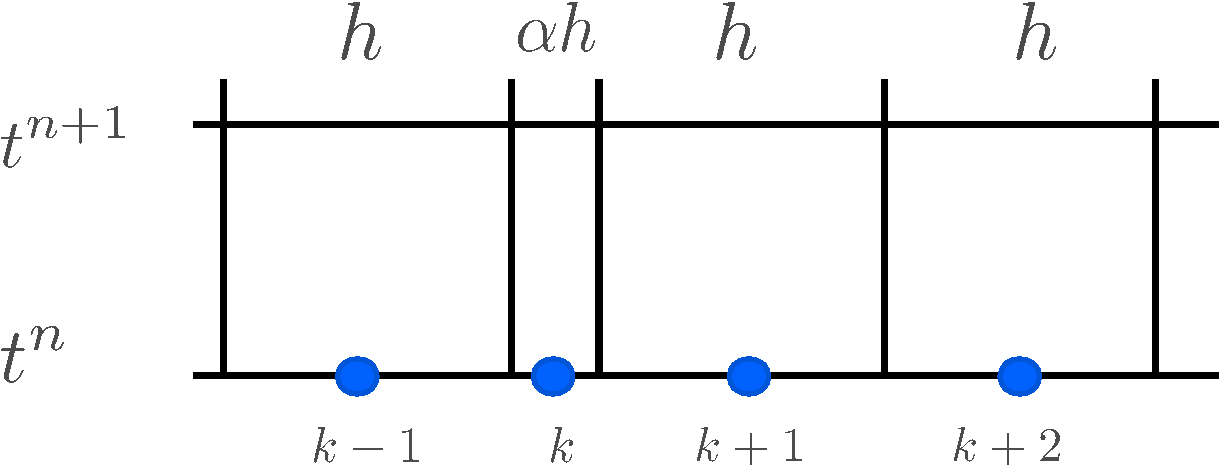
\includegraphics[height=1.3in]{figs/1dfig.pdf}
\caption{\sf Notation for model problem in one space dimension. The small
cell has size $\alpha h$ in a mesh with regular mesh width $h$.}
\label{fig:modelProblem1}
\end{center}
\end{figure}

To set the stage, notice that cell merging can
be rewritten as a postprocessing step.
To take one step to update a finite volume approximation to
$u_t + u_x = 0$ we do the following:
\begin{itemize}
\setlength\itemsep{.2in}
\item
{\bf Finite Volume Step}\\
Take the usual finite volume step with fixed, regular  $\Delta t$ on all cells 
including the small cell:
\begin{equation}
\bar{u}_j = u_j^n - \frac{\Delta t}{h_j} \; (f_{j+1/2} - f_{j-1/2} ), 
\quad \forall j.
\label{eqn:fvupdate}
\end{equation}

\item
{\bf {\em Temporarily} Create Merged Cell}\\
Temporarily create the {\em merged} cell $\overline{u_M}$ consisting of the small cell $u_j$ and one
or both of its neighbors so that it the merged cell is of sufficient
size (to be discussed later).  For simplicity here we will merge 
only with the neighbor on the right,
\begin{equation}
\widehat{u_M} =  \frac{ h_k \bar{u}_k + h_{k+1} \bar{u}_{k+1} } {h_k +
h_{k+1}} .
\label{eqn:mergestep}
\end{equation}

\item
{\bf Compute Merge Cell Gradient }\\
There are several ways to do this. 
\ref{sec:srdAlg}.
Two simple possibilities are 
\begin{equation}
\nabla \widehat{u_M} = \frac{\bar{u}_{k+2} - \bar{u}_{k-1}} {x_{k+2}-x_{k-1}}
\label{eqn:gradLim1}
\end{equation}
which does not use the merged cell,
or
\begin{equation}
\nabla \widehat{u_M} = \frac{\bar{u}_{k+2} - \widehat{u_{M}}} {x_{k+2}-x_{M}}
\label{eqn:gradLim2}
\end{equation}
which uses the merged cell, and $x_M$ is the centroid of the merged
cell.
The choice of gradient stencil will be studied later. 

%Other more accurate alternatives exist, not all of which are stable.
%It would be better to use smaller stencils, perhaps including $u_{k+1}$
%or $\overline{u_M}$ itself.

\item
{\bf Redistribute Merged State to Cells Comprising Merged cell }\\
Replace the provisional values computed in the cells comprising the
merged cell with the merged solution reconstructed to the cell
centroids:
\begin{equation}
\begin{split}
u_k^{n+1} &= \widehat{u_M} +  (x_k - x_M) \nabla \widehat{u_M}\\
u_{k+1}^{n+1} &= \widehat{u_M} +  (x_{k+1} - x_M) \nabla \widehat{u_M}
\end{split}
\end{equation}
\end{itemize}
This method is clearly linearity preserving if all gradients are
computed accurately enough to preserve a linear function.  
It is conservative since the mass of the merged cell equals the mass of
the two cells comprising it, and the linear function through the
centroid also has the same amount of total mass.

When written in one-step form instead of as a post-processing step, 
it is seen to be closely related to cell merging. 
In the first order case without gradient, the above gives
\begin{equation}
u_k^{n+1} = u_{k+1}^{n+1} = \widehat{u_M}^{n+1} 
\end{equation}
Pluging in the updates for $\widehat{u_M}$ we get
\begin{equation}
\widehat{u_M}^{n+1} = \widehat{u_M}^n - 
\frac{\Delta t}{h_k + h_{k+1}} (f_{k+3/2} - f_{k-1/2})
\end{equation}
Recognizing that $h_k+h_{k+1}$ is the merged cell volume makes this
clear.
By using a higher than linear polynomial and
including more neighbors in the
redistribution (on top of a more accurate scheme for the entire grid),
we have a path to higher order accuracy.
%By including gradients it provides a path to higher dimensions, possibly 
%overlapping neighborhoods. 

The choice of merging neighborhoods and gradients is what makes up the
specifics of SRD in two space dimensions. Furthermore, it can happen
that a cell has more than one neighborhood with
which it should merge. This is what often causes complications in cell
merging algorithms. In SRD, we will simply use all such values appropriately
weighted.

In the next section we present the SRD algorithm in two dimensions.
For simplicity we present the second order accurate version first.
The more general higher order extension is described in 
section \ref{sec:ho}.
Some theoretical results using one-dimensional model problems are in
section \ref{sec:theory}. 
Section \ref{sec:compResults} shows computational results for both smooth
problems and shocked flow for both linear advection and the Euler equations.  We conclude in section \ref{sec:conc}.

\section{State redistribution in one dimension} \label{sec:srd1d}
We begin this section  by reminding the reader that cell merging can
be written as a postprocessing step. We then show that the extension of
cell merging for overlapping cells does not maintain conservation. 
This motivates our state redistribution approach, which we contrast with
cell merging on a simple one dimensional example. 
Although the small cells do not mimic the cut cells at the 
boundary in higher dimensions, this is still a useful model problem. 

For the examples in this section we will solve the linear advection equation
\begin{equation}\label{eq:hpde}
u_t + au_x = 0, \quad a>0
\end{equation}
on a nonuniform grid, called the base grid. Equation \eqref{eq:hpde} is
discretized  using the  first order
accurate upwind scheme 
\begin{equation}\label{eq:unstable1d}
\widehat{U}_i = U^n_i - \frac{a \Delta t} {h_i} \, (U^n_i -U^n_{i-1}),
\end{equation}
where $U^n_i$ is the solution average on cell $i$ at time $t^n$, the time
step $\Delta t$ is constant for all cells. On full cells $h_i = h$, and on
the small cells  $h_i = \alpha h$ for $ 0 < \alpha < 1$.
We first use
the grid in Figure \ref{fig:ng1}(a) with one small cell at $i=0$, then the grid
in Figure \ref{fig:ng1}(b) with two small cells at $i = -1$ and $1$.

\begin{figure}[h]
\centering
\vspace*{.2in}
\mbox{
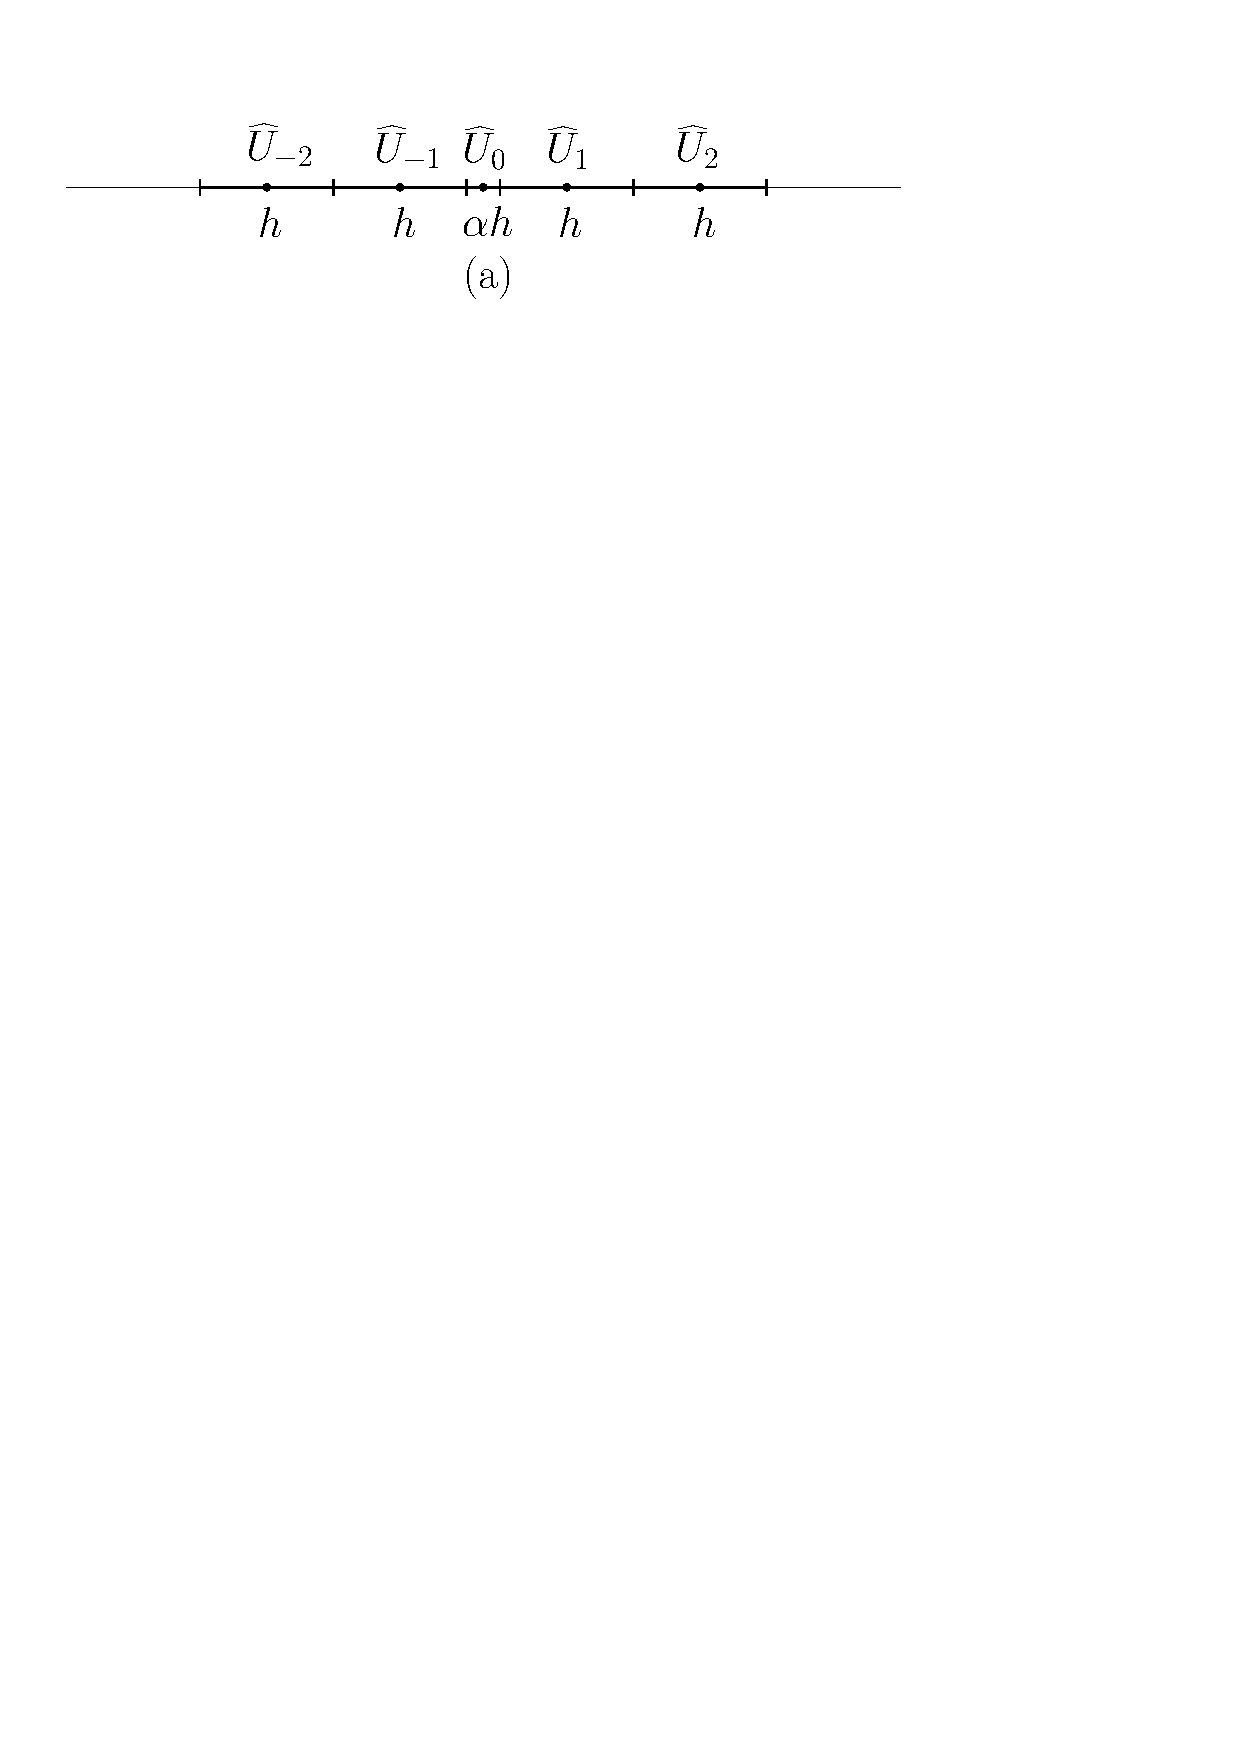
\includegraphics[width=0.4\linewidth,trim=30 0 20 0,clip]{figs/overlapping_simple.pdf} 
\hspace*{.1in}
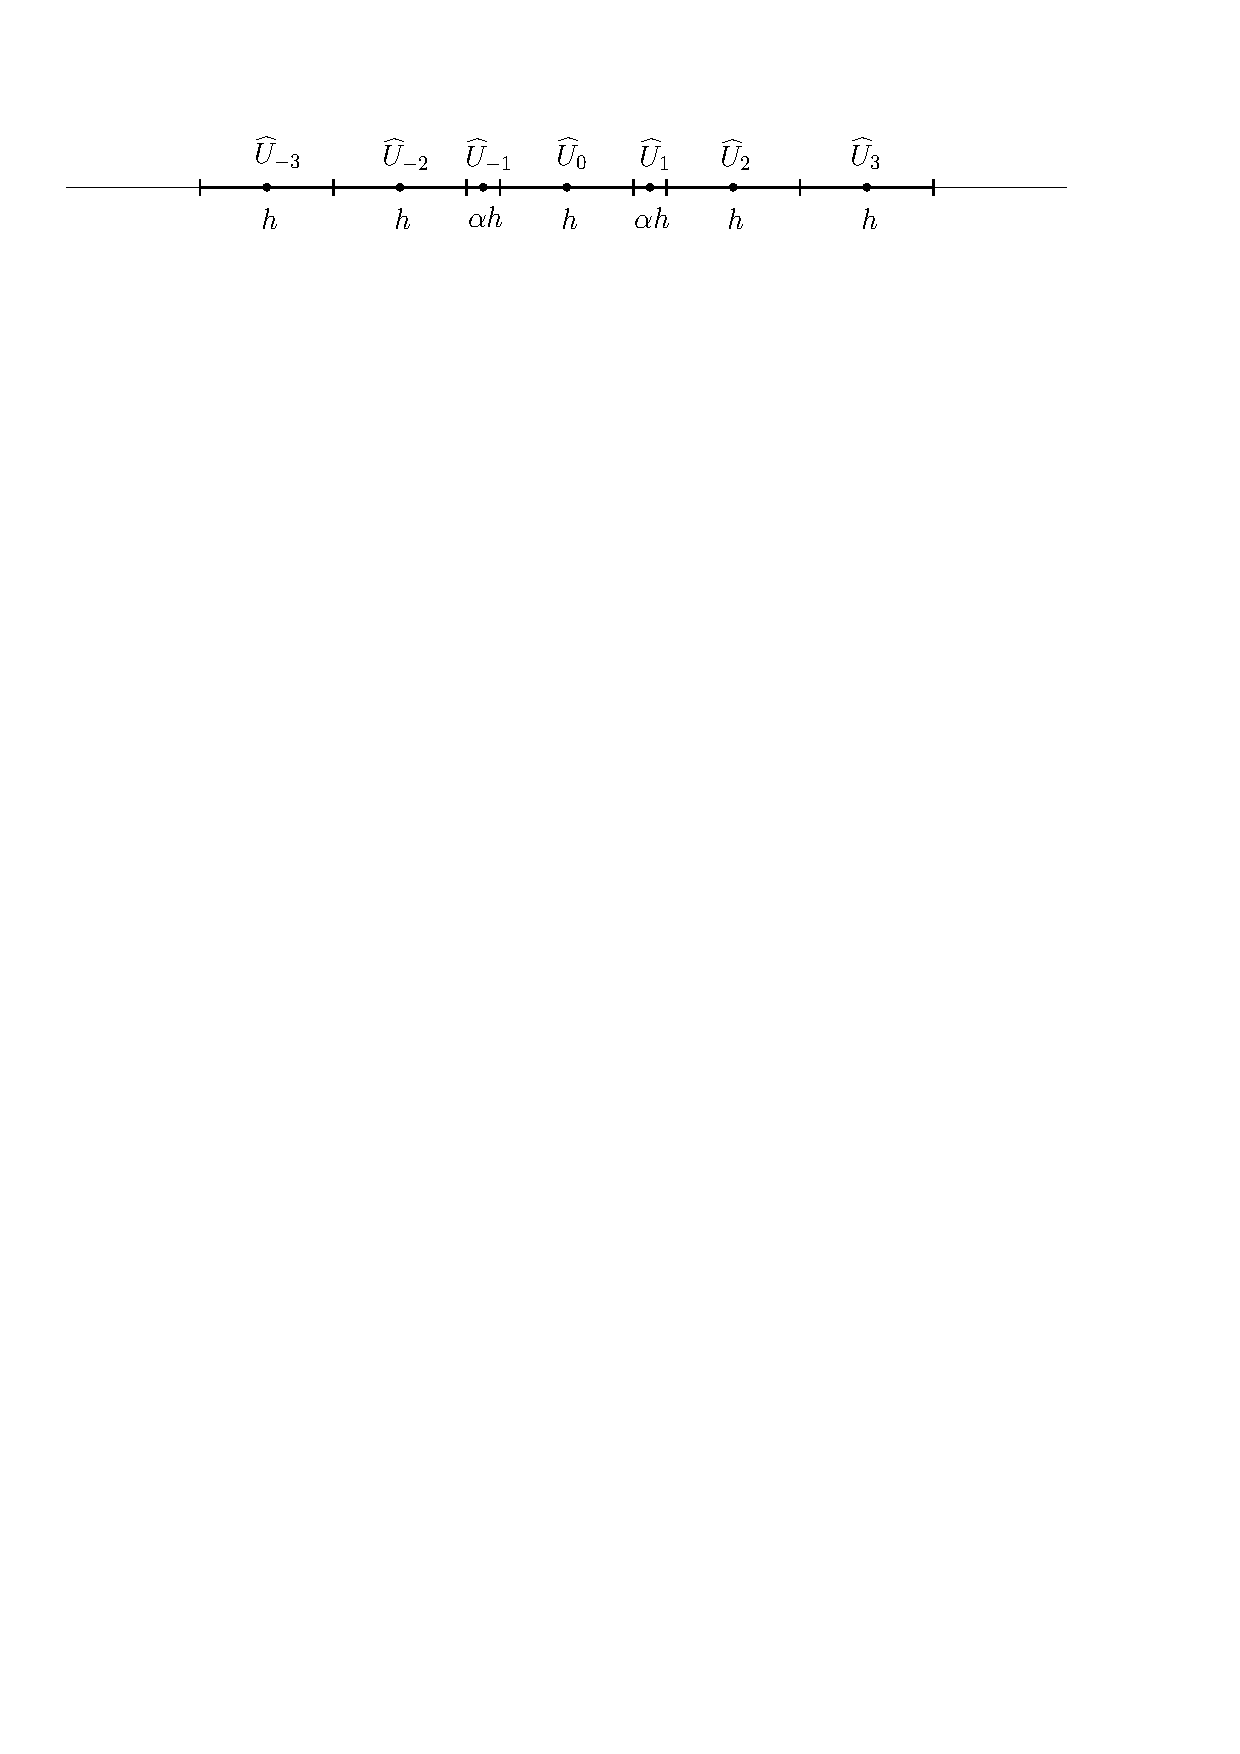
\includegraphics[width=0.5\linewidth,trim=15 0 25 0,clip]{figs/overlapping.pdf}
}
\vspace*{.1in}
\caption{\sf Model problem in one space dimension on a nonuniform base grid.
On the left there is one small cell at $i=0$. The right grid has two small 
cells  at $i = -1$ and $1$.  The small and large cell 
sizes are $\alpha h$ ($0<\alpha < 1$), and $h$, respectively. \label{fig:ng1}}
\end{figure}

On the grid in Figure \ref{fig:ng1}(a), cell merging might 
group cells -1,0, and 1 together into a larger, merged cell.
After the unstable update in \eqref{eq:unstable1d}, the  volume-weighted
merged cell average $\widehat{Q}_0$ is computed:
\begin{equation}
\widehat{Q}_0 = \frac{\widehat{U}_{-1} + \alpha \,  \widehat{U}_0 + 
\widehat{U}_1}{2+\alpha} .
\end{equation}
The cells comprising the merged cell
are then replaced by $\widehat{Q}_0$:
\begin{equation}
\widehat{U}_{-1}^{n+1} = \widehat{U}_0^{n+1} = \widehat{U}_1^{n+1} =
\widehat{Q}_0
\end{equation}
This is easily seen to be conservative by checking that
\begin{equation}
\underbrace{h \, (U_{-1}^{n+1} + \alpha \, U_0^{n+1} +
U_1^{n+1})}_{\text{mass after redistribution}}
= (2+\alpha) h \,  \, \widehat{Q}_0 =
\underbrace{ h \, (\widehat{U}_{-1} + \alpha \, \widehat{U}_{0} +
\widehat{U}_{1})}_{\text{mass before redistribution}}
\end{equation}
which equals the values at time $t^n$  except for the mass entering and
leaving this region.


Next, consider the more complicated case of Figure \ref{fig:ng1}(b).
Five cells (indexed by $-3$, $-2$, $0$, $2$, $3$) are large 
with size $h$ and the remaining two cells (indexed by $-1$ and $1$) 
are small with size $\alpha h$.
A first approach to cell merging on this grid
might be to make two merged cell averages, $\widehat{Q}_{-1}$
comprising cells ${-2},{-1},0$, and $\widehat{Q}_1$ comprising cells
$0, 1$ and $2$, associated respectively with the small cells $-1$ and $1$.
The first order version here would assign cells as before, except that
since cell 0 belongs to two neighborhoods, it seems  reasonable
to assign $U_0^{n+1} = \frac{1}{2} (\widehat{Q}_{-1} + \widehat{Q}_1).$  
To check for conservation, we again compute the sum
\begin{equation}
\begin{split}
\underbrace{h \, (U_{-2}^{n+1} + \alpha\,U_{-1}^{n+1} + U_0^{n+1} + \alpha \, U_1^{n+1}
+ U_2^{n+1})}_{\text{mass after redistribution}} = \\[.1in]
h \left [(1+\alpha +1/2) \, \widehat{Q}_{-1} +
 (1/2+\alpha +1) \, \widehat{Q}_{1}\right ]  = \\[.1in]
h \,  (3/2+\alpha) \, \left [ \frac{(\widehat{U}_{-2} + \alpha \widehat{U}_{-1} +
\widehat{U}_0)}{2+\alpha} +
        \frac{(\widehat{U}_{0} + \alpha \widehat{U}_{1} 
        + \widehat{U}_2)}{2+\alpha} \right ]  \neq \\[.08in]
\underbrace{h \,  ( \widehat{U}_{-2} + \alpha \widehat{U}_{-1} +
\widehat{U}_0 +  \alpha \widehat{U}_{1} + 
\widehat{U}_2 )}_{\text{mass before redistribution}}.  
\end{split}
\end{equation}
So at least this extension of cell merging to overlapping cells is not
conservative.

This motivates the state redistribution
procedure, which allows for overlapping cells and stabilizes 
$\widehat{U}_i$ in a conservative manner.
This is done by temporarily merging cells of the grid into 
larger, possibly overlapping, neighborhoods using a specially weighted 
convex combination, and recombining these averages back onto the
grid in a particular fashion.  These merged cells are 
constructed once during a mesh preprocessing step before time stepping.

\begin{figure}[h]
\begin{center}
\vspace*{.1in}
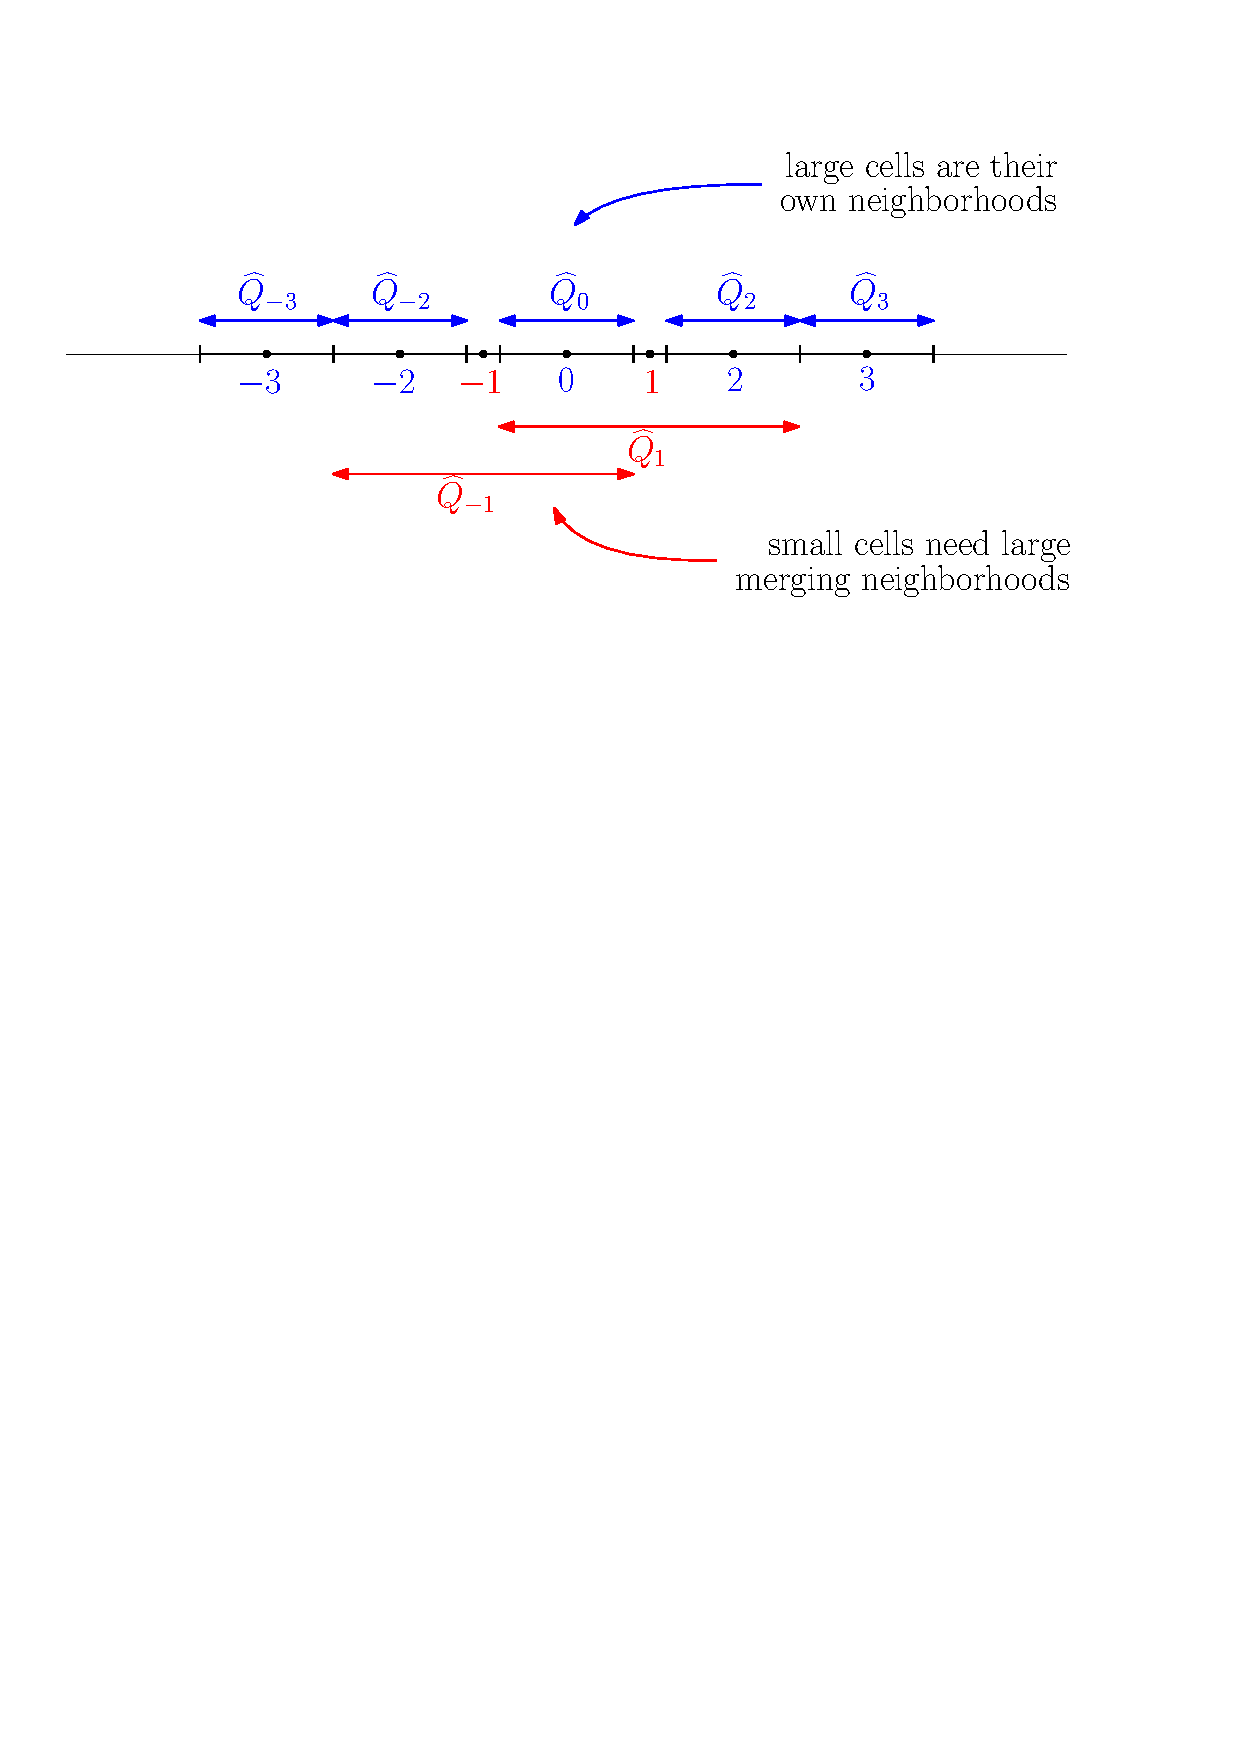
\includegraphics[width=0.75\linewidth]{figs/overlapping1.pdf} 
\caption{\sf 
The blue arrows indicate the merging neighborhoods associated with the large 
cells $-3$, $-2$, $0$, $2$, and $3$, which are their own neighborhoods.  
The red arrows indicate the neighborhoods of small cells $-1$ and $1$, which
have temporarily merged with their left and right neighbors.  
%The numbers next to the arrows are the neighborhood index, which
%correspond to the cell indices in Fig. \ref{fig:ng1}.  
\label{fig:mn1}}
\end{center}
\end{figure}

\subsubsection*{State redistribution preprocessing}
Each cell in the base grid (both large and small) has a merging neighborhood
associated with it.
This is  a set of neighboring cells with which to temporarily merge.
Neighborhoods share the same index as the cell that generated it.
%The merging neighborhood associated with cell $i$ is called $M_i$. 
Small cells merge with their neighbors until the volume of the merging neighborhood is greater than
a threshold, taken here to be half the large cell size of $h/2$.
This is illustrated by the red arrows in Figure \ref{fig:mn1} where the merging neighborhood of 
small cell $-1$ consists of cells $-2$, $-1$, and $0$, and the merging neighborhood of 
small cell 1 consists of cells $0$, $1$, and $2$. 
Note that   both neighborhoods overlap on cell 0. Allowing
for overlaps makes this temporary merging process simpler.
A large cell does not need to merge with neighbors (since $h > h/2$), thus its merging neighborhood is only 
composed of itself.  This is illustrated by the blue arrows in Figure
\ref{fig:mn1}. For example,  the 
merging neighborhood of large cell $-3$ is composed only of itself.

Finally, each cell in the base grid counts the number of neighborhoods that overlap it. 
Cell $-2$ is overlapped by two neighborhoods, indexed by $-1$ and $-2$.
Cell 0 has 3 such neighborhoods, its own, and one from each small cell adjacent to it.

\subsubsection*{State redistribution postprocessing}
Using the above information we can now stabilize \eqref{eq:unstable1d} using the state redistribution 
method on the grid in Figure \ref{fig:ng1}b.  
On each merging neighborhood, we compute a weighted solution average $\widehat Q_i$, where $i$ is the 
index of the merging neighborhood. 
$\widehat Q_i$ is computed by a convex combination of the averages $\widehat{U}_i$ of cells contained in the 
merging neighborhood, weighted by the inverse of its overlap count. 
For example, on merging neighborhood $-1$, the weighted solution average is
\begin{equation}\label{eq:neigh2}
\widehat{Q}_{-1} = \frac{1}{\underbrace{h/2 + \alpha h + h/3}_{\text{weighted volume}}}\biggr( \underbrace{\frac{h}{2} \widehat{U}_{-2} + \alpha h \widehat{U}_{-1} + \frac{h}{3}\widehat{U}_{0}}_{\text{weighted mass}} \biggr).
\end{equation}
In formula \eqref{eq:neigh2}  for the weighted mass,
the cell volume is divided by the number of neighborhoods that overlap the associated cell 
in the base grid. 
For example, the multiplier in front of $\widehat{U}_{-2}$ is $\frac{h}{2}$ since there are 
two neighborhoods (from cells $-1$ and $-2$) that overlap cell $-2$.  
Similarly, the multiplier in front of $\widehat{U}_{-1}$ is $\alpha h$ since there is only 
one neighborhood (its own) that overlaps cell $-1$.
Finally, the multiplier in front of $\widehat{U}_{0}$ is $\frac{h}{3}$ since there are three neighborhoods that overlap cell $0$, i.e., cell $0$ is overlapped by neighborhoods $-1$, $1$, and $0$.
These multipliers are then divided by the weighted volume,  $(h/2 + \alpha h + h/3)$.
%since $\widehat{Q}_{-1} $ must be a convex combination of $\widehat{U}_{-2}$, $\widehat{U}_{-1}$, and $\widehat{U}_{0}$.
The weighted solution average on merging neighborhood $1$ is similarly defined as
\begin{equation}\label{eq:neigh3}
\widehat{Q}_{1} = \frac{1}{h/2 + \alpha h + h/3}\left( \frac{h}{2} \widehat{U}_{2} + \alpha h \widehat{U}_{1} + \frac{h}{3}\widehat{U}_{0} \right).
\end{equation}
The weighted solution averages on merging neighborhoods that contain only one cell are simply 
\begin{equation}\label{eq:neigh1}
\widehat{Q}_i = \widehat{U}_i \quad \text{ for } i = -3,-2,0,2,3.
\end{equation}

The stabilized solution average at time $t^{n+1}$ on a cell in the base grid is then 
given by the average of all the weighted neighborhood averages that overlap it.  
On the cell overlapped by three neighborhoods we have
\begin{equation} \label{eq:threeneigh}
U^{n+1}_{0} = \frac{1}{3}(\widehat{Q}_{-1}+\widehat{Q}_{0}+\widehat{Q}_{1}).
\end{equation}
On the  cells overlapped by two neighborhoods, we have
\begin{equation} \label{eq:twoneigh}
U^{n+1}_{-2} = \frac{1}{2}(\widehat{Q}_{-1}+\widehat{Q}_{-2}) \text{ and } U^{n+1}_{2} = \frac{1}{2}(\widehat{Q}_{1}+\widehat{Q}_{2}).
\end{equation}
Finally, on cells overlapped by only one neighborhood,  we have
\begin{equation} \label{eq:oneneigh}
	U^{n+1}_i = \widehat{Q}_i \text{ for } i = -3,-1,1,3.
\end{equation}

We can write the final solution update on the small cells after SRD  at $t^{n+1}$ in terms of the solution 
averages at $t^{n}$, giving
\begin{equation}
\begin{aligned}
U^{n+1}_{-1} &= \frac{2-2\lambda}{5+6\alpha}U^n_0 + \frac{6\alpha - 4 \lambda}{5+6\alpha}U^n_{i-1}+ \frac{3\lambda + 3}{5+6\alpha}U^n_{i-2}+\frac{3\lambda }{5+6\alpha}U^n_{i-3}, \\
U^{n+1}_{1} &= \frac{2+4\lambda}{5+6\alpha}U^n_0 + \frac{6\alpha - 3 \lambda}{5+6\alpha}U^n_{i+1}+ \frac{3-3\lambda}{5+6\alpha}U^n_{i+2}+\frac{2\lambda }{5+6\alpha}U^n_{i-1}.
\end{aligned} \label{eq:finalupdate}
\end{equation}
Before application of the state redistribution method, the weights that multiply the solution averages at time $t^n$ in the base scheme \eqref{eq:unstable1d} become unbounded as $\alpha \rightarrow 0$.
However, after state redistribution this is no longer the case for the weights 
in \eqref{eq:finalupdate}.  This hints at the stability of our modified scheme.  

The state redistribution algorithm allows us to take full time steps as if there were no 
small cells in the grid.  However, it can be seen that the multipliers of $U^n_{i-1}$ and $U^n_{i+1}$ 
in \eqref{eq:finalupdate} are negative when $\alpha$ is small enough.  This means that our scheme is not 
monotone and is also not total variation diminishing (TVD). However TVD is
not possible in many cases of interest.  In particular, we note that this is 
also the case 
with flux redistribution, which has been successfully used in higher dimensions and more
complicated problems.  
The computational examples in Section \ref{sec:compResults} show that
this is not a significant issue for SRD as well.
The advantage of state redistribution  is that it is linearity
preserving, and flux redistribution is not. 

\subsubsection*{Conservation}
We now show that our modified scheme \eqref{eq:threeneigh}, \eqref{eq:twoneigh}, \eqref{eq:oneneigh} conserves mass.
%, i.e., the total mass of the numerical solution before and after state redistribution is the same.  
For the portion of the grid in question, the total mass after state redistribution is
\begin{equation}\label{eq:tm1}
	\sum_{i} h_i U^{n+1}_i  = h U^{n+1}_{-3} + h U^{n+1}_{-2} + \alpha h U^{n+1}_{-1} +h U^{n+1}_0+\alpha h U^{n+1}_{1} + h U^{n+1}_{2} + h U^{n+1}_{3},
\end{equation}
where $h_i$ is the local cell size.
%i.e., $h_i = \alpha h$ for $i \neq -1,1$ and $h_i = h$ otherwise.
Substituting expressions for the final update \eqref{eq:threeneigh}, \eqref{eq:twoneigh}, \eqref{eq:oneneigh} into \eqref{eq:tm1}, we obtain
\begin{equation}\label{eq:tm2}
\begin{aligned}
\sum_{i} h_i U^{n+1}_i  &= h \widehat{Q}_{-3} + \frac{h}{2}(\widehat{Q}_{-1}+\widehat{Q}_{-2}) \\
&+ \alpha h \widehat{Q}_{-1} +h \frac{1}{3}(\widehat{Q}_{-1}+\widehat{Q}_{0}+\widehat{Q}_{1})+\alpha h \widehat{Q}_{1} \\
&+ h \frac{1}{2}(\widehat{Q}_{1}+\widehat{Q}_{2}) + h \widehat{Q}_{3}.
\end{aligned}
\end{equation}
Grouping terms in \eqref{eq:tm2}, we have
\begin{equation}\label{eq:tm3}
\begin{aligned}
\sum_{i} h_i U^{n+1}_i  &= h \widehat{Q}_{-3} + \frac{h}{2}\widehat{Q}_{-2} \\
&+ \left(\frac{h}{2}+\alpha h + \frac{h}{3}\right) \widehat{Q}_{-1} + \frac{h}{3} \widehat{Q}_0 + \left(\frac{h}{2}+\alpha h + \frac{h}{3}\right) \widehat{Q}_{1} \\
&+ \frac{h}{2}\widehat{Q}_{2} + h \widehat{Q}_3.
\end{aligned}
\end{equation}
Substituting the expressions for the neighborhood averages \eqref{eq:neigh3}, \eqref{eq:neigh2}, \eqref{eq:neigh1} into \eqref{eq:tm3}, we obtain
\begin{equation}\label{eq:tm4}
\begin{aligned}
\sum_{i} h_i U^{n+1}_i  &= h \widehat{U}_{-3} + \frac{h}{2}\widehat{U}_{-2} \\
&+ \left(\frac{h}{2} \widehat{U}_{-2} + \alpha h \widehat{U}_{-1} + \frac{h}{3}\widehat{U}_{0}\right) + \frac{h}{3} \widehat{U}_0 + \left(\frac{h}{2} \widehat{U}_{2} + \alpha h \widehat{U}_{1} + \frac{h}{3}\widehat{U}_{0}\right) \\
&+ \frac{h}{2}\widehat{U}_{2} + h \widehat{U}_3.
\end{aligned}
\end{equation}
Simplifying \eqref{eq:tm4}, the mass after state redistribution becomes
\begin{equation}\label{eq:tm5}
\begin{aligned}
\sum_{i} h_i U^{n+1}_i  &= h \widehat{U}_{-3} + h \widehat{U}_{-2} + \alpha h \widehat{U}_{-1} +h \widehat{U}_0+\alpha h \widehat{U}_{1} + h \widehat{U}_{2} + h \widehat{U}_{3},\\
&= \sum_{i} h_i \widehat{U}_i.
\end{aligned}
\end{equation}
Thus, the mass on the grid before and after state redistribution does not change.
Since the base scheme \eqref{eq:unstable1d} is conservative, it follows from
\eqref{eq:tm5} that our modified scheme \eqref{eq:threeneigh},
\eqref{eq:twoneigh}, \eqref{eq:oneneigh} is too.
%, our modified scheme \eqref{eq:threeneigh}, \eqref{eq:twoneigh}, \eqref{eq:oneneigh} is conservative.  
%Thus, the base scheme coupled with the state redistribution method is conservative.  




The stabilized finite volume method \eqref{eq:threeneigh},
\eqref{eq:twoneigh}, \eqref{eq:oneneigh} is first order accurate in space
and time.  In this work, we provide a framework to generalize the state
redistribution method to two dimensional cut cell grids and to 
second order accuracy in space and time.
We will demonstrate with numerical examples that the maximum stable time step is 
not restricted by the small cells, and that the state redistribution method 
is conservative.



%In the next section  we discuss the base finite volume schemes that will be stabilized by state redistribution.


%\subsubsection*{Weighted volume of merging neighborhood}
%Each merging neighborhood has an associated a weighted volume




%\begin{equation}
%	\widehat{V}_i = \sum_{i \in M_i} \frac{h}{den}
%\end{equation}

%\subsubsection*{Solution average on merging neighborhood}
%We compute a weighted solution average on each merging neighborhood, $M_i$, using the following formula
%\begin{equation}\label{eq:merging}
%	\widehat{Q}_{i} = 
%\end{equation}



%The merging cell consists consisting of the small cell $u_j$ and one or both of its neighbors so that it the merged cell is of sufficient

%\begin{figure}
%	\subfloat[$50\times50$ grid and annulus domain.]{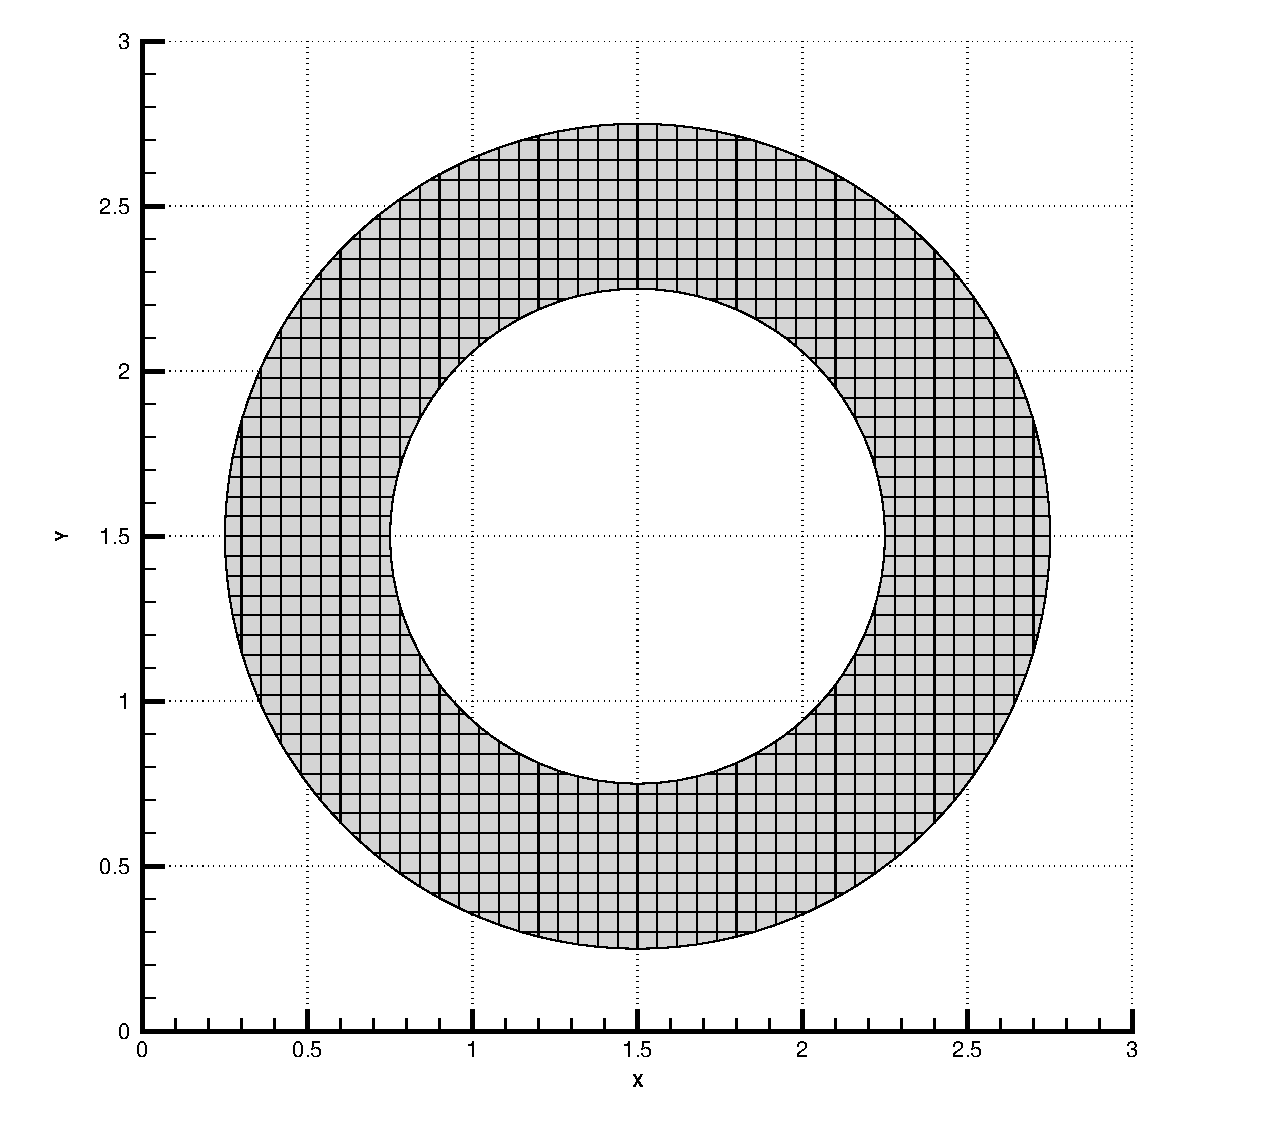
\includegraphics[width = 0.5\linewidth]{figs/rotatinghill_grid.eps} \label{fig:rotatinghillgrid}} 
%	\quad
%	\subfloat[Isolines of exact solution at the initial and final time. SHOW
%	COMPUTED SOLUTION TOO]{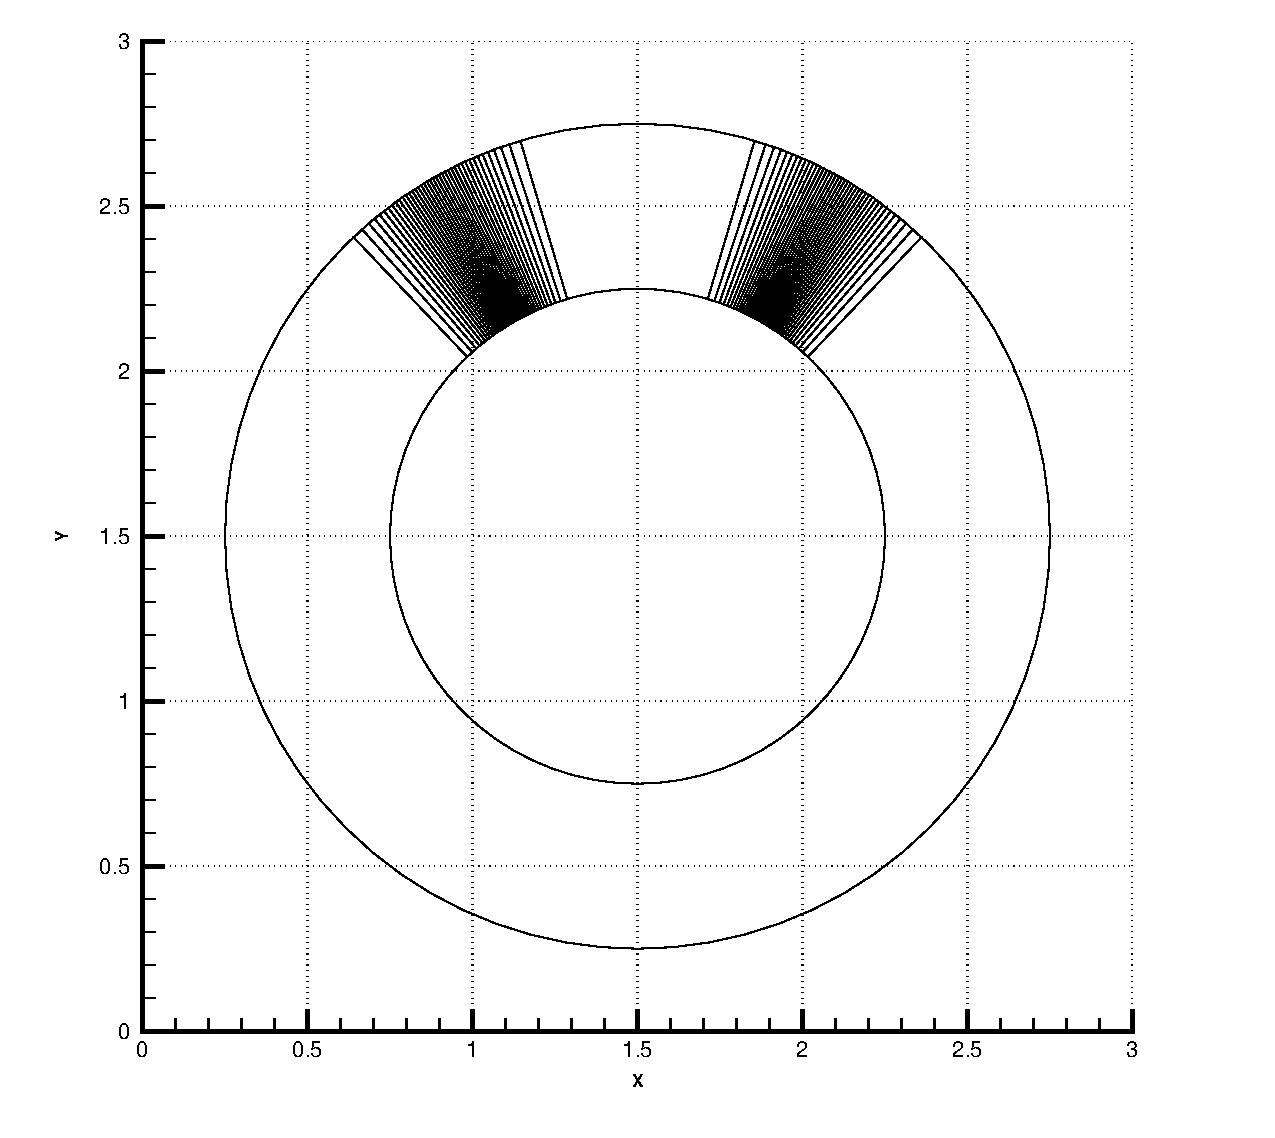
\includegraphics[width = 0.5\linewidth]{figs/rotatinghill_solution.eps}\label{fig:rotatinghillexactiso}}
%\end{figure}
%\begin{figure}
%	\begin{center}
%		%\vspace*{-.5in}
%		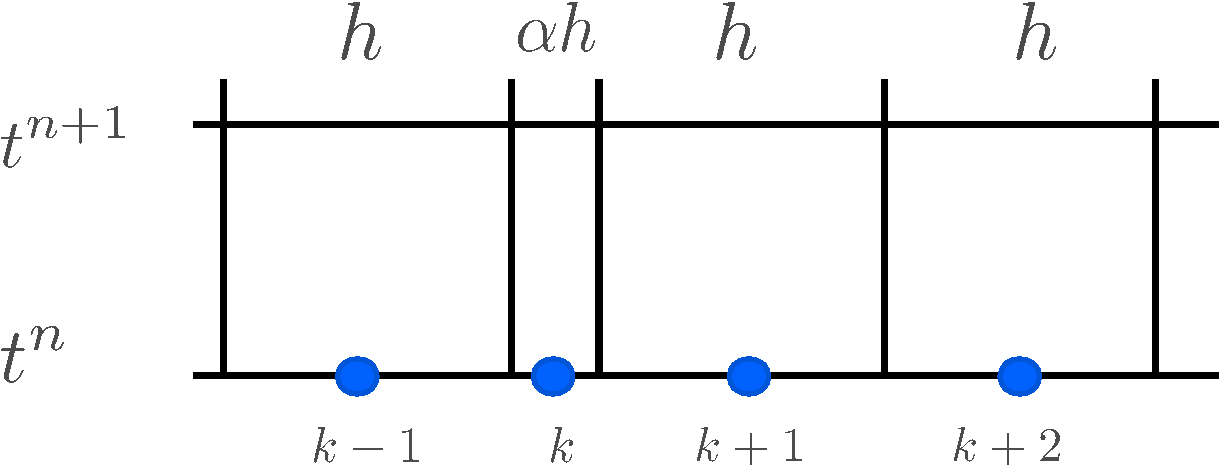
\includegraphics[height=1.3in]{figs/1dfig.pdf}
%		\caption{\sf Notation for model problem in one space dimension. The small
%			cell has size $\alpha h$ in a mesh with regular mesh width $h$.}
%		\label{fig:modelProblem1}
%	\end{center}
%\end{figure}


%To set the stage, notice that cell merging itself can
%be rewritten as a postprocessing step.
%\commentout{
%To take one step to update a finite volume approximation to
%$u_t + u_x = 0$ we do the following:
%\begin{itemize}
%\setlength\itemsep{.2in}
%\item
%{\bf Finite Volume Step}\\
%Take the usual finite volume step with fixed, regular  $\Delta t$ on all cells 
%including the small cell:
%\begin{equation}
%\bar{u}_j = u_j^n - \frac{\Delta t}{h_j} \; (f_{j+1/2} - f_{j-1/2} ), 
%\quad \forall j.
%\label{eqn:fvupdate}
%\end{equation}
%
%\item
%{\bf {\em Temporarily} Create Merged Cell}\\
%Temporarily create the {\em merged} cell $\overline{u_M}$ consisting of the small cell $u_j$ and one
%or both of its neighbors so that it the merged cell is of sufficient
%size (to be discussed later).  For simplicity here we will merge 
%only with the neighbor on the right,
%\begin{equation}
%\widehat{q_M} =  \frac{ h_k \bar{u}_k + h_{k+1} \bar{u}_{k+1} } {h_k +
%h_{k+1}} .
%\label{eqn:mergestep}
%\end{equation}
%
%\item
%{\bf Compute Merge Cell Gradient }\\
%There are several ways to do this. 
%Two simple possibilities are 
%\begin{equation}
%\nabla \widehat{u_M} = \frac{\bar{u}_{k+2} - \bar{u}_{k-1}} {x_{k+2}-x_{k-1}}
%\label{eqn:gradLim1}
%\end{equation}
%which does not use the merged cell,
%or
%\begin{equation}
%\nabla \widehat{u_M} = \frac{\bar{q}_{k+2} - \widehat{u_{M}}} {x_{k+2}-x_{M}}
%\label{eqn:gradLim2}
%\end{equation}
%which uses the merged cell, and $x_M$ is the centroid of the merged
%cell.
%The choice of gradient stencil will be studied later in section \ref{sec:srdAlg}.
%
%%Other more accurate alternatives exist, not all of which are stable.
%%It would be better to use smaller stencils, perhaps including $u_{k+1}$
%%or $\overline{u_M}$ itself.
%
%\item
%{\bf Redistribute Merged State to Cells Comprising Merged cell }\\
%Replace the provisional values computed in the cells comprising the
%merged cell with the merged solution reconstructed to the cell
%centroids:
%\begin{equation}
%\begin{split}
%u_k^{n+1} &= \widehat{u_M} +  (x_k - x_M) \nabla \widehat{u_M}\\
%u_{k+1}^{n+1} &= \widehat{u_M} +  (x_{k+1} - x_M) \nabla \widehat{u_M}
%\end{split}
%\end{equation}
%\end{itemize}
%}
%First update cells $k$ and $k+1$, shown in Figure \ref{fig:modelProblem1},  using a 
%standard finite volume scheme on all cells:
%\begin{equation}
%\bar{u}_j = u_j^n - \frac{\Delta t}{h_j} \; (f_{j+1/2} - f_{j-1/2} ), 
%\quad \forall j.
%\label{eqn:fvupdate}
%\end{equation}
%Next form the merged cell
%\begin{equation}
%\widehat{q_M} =  \frac{ h_k \bar{u}_k + h_{k+1} \bar{u}_{k+1} } {h_k +
%h_{k+1}} .
%\label{eqn:mergestep}
%\end{equation}
%which works out to
%\begin{equation}
%\widehat{q_M} = \widehat{q_M}^n - 
%\frac{\Delta t}{h_k + h_{k+1}} (f_{k+3/2} - f_{k-1/2})
%\end{equation}
%For the simplest first order version, we simply set
%\begin{equation}
%u_k^{n+1} = u_{k+1}^{n+1} = \widehat{q_M} 
%\label{eqn:finalstep}
%\end{equation}
%Recognizing that $h_k+h_{k+1}$ is the merged cell volume makes 
%clear the relationship to cell merging.
%The final update step \eqref{eqn:finalstep} is replaced by 
%\begin{equation}
%\begin{split}
%u_k^{n+1} &= \widehat{q_M} +  (x_k - \widehat{x}_M) \,\,  \widehat{\sigma_M}\\
%u_{k+1}^{n+1} &= \widehat{q_M} +  (x_{k+1} - \widehat{x}_M) \,  \widehat{\sigma_M}
%\end{split}
%\end{equation}
%where $\widehat{\sigma_M}$ is a reconstructed slope on the merged cell.
%The state redistribution method is linearity preserving when the base finite volume scheme and the reconstructed slope on merged cells $\widehat{\sigma_M}$ are accurate enough.
%By using a polynomial of degree $d>1$ and
%including more neighbors in the
%redistribution (on top of a more accurate finite volume scheme for the
%entire mesh),
%we have a path to higher order accuracy.
%The method is also conservative since the mass of the merged cell equals the 
%mass of the two cells comprising it.



%The choice of merging neighborhoods and gradients is what makes up the
%specifics of SRD in two space dimensions. Furthermore, it can happen
%that a cell has more than one neighborhood with
%which it should merge. This is what often causes complications in cell
%merging algorithms. In SRD, we will simply use all such values appropriately
%weighted.
%
%In the next section  we first discuss the finite volume schemes to which SRD will
%be applied.
%The SRD algorithm in two space dimensions will be presented in section
%\ref{sec:srdAlg}.
%For simplicity we present the second order accurate version first.
%The more general higher order extension is described in 
%section \ref{sec:ho}.
%Some theoretical results using one-dimensional model problems are in
%section \ref{sec:theory}. 
%Section \ref{sec:compResults} shows computational results for both smooth
%problems and shocked flow for both linear advection and the Euler equations.  We conclude in section \ref{sec:conc}.

\section{Base Finite Volume Schemes}\label{sec:basefv}

Our computational results will use two different finite volume schemes
to update the Cartesian cut cell mesh, to show that SRD can be used in a
variety of situations.
We will refer to these at the base schemes. 
The  update is applied to the entire mesh, including  
to the small cut cells.  Since cut cells can have cell volumes that are
orders of magnitude smaller than the time step allowed by the full
cells, these will lead to instability without a stabilization algorithm.
SRD will be applied after each stage or step of the base scheme.

\begin{figure}
\begin{center}
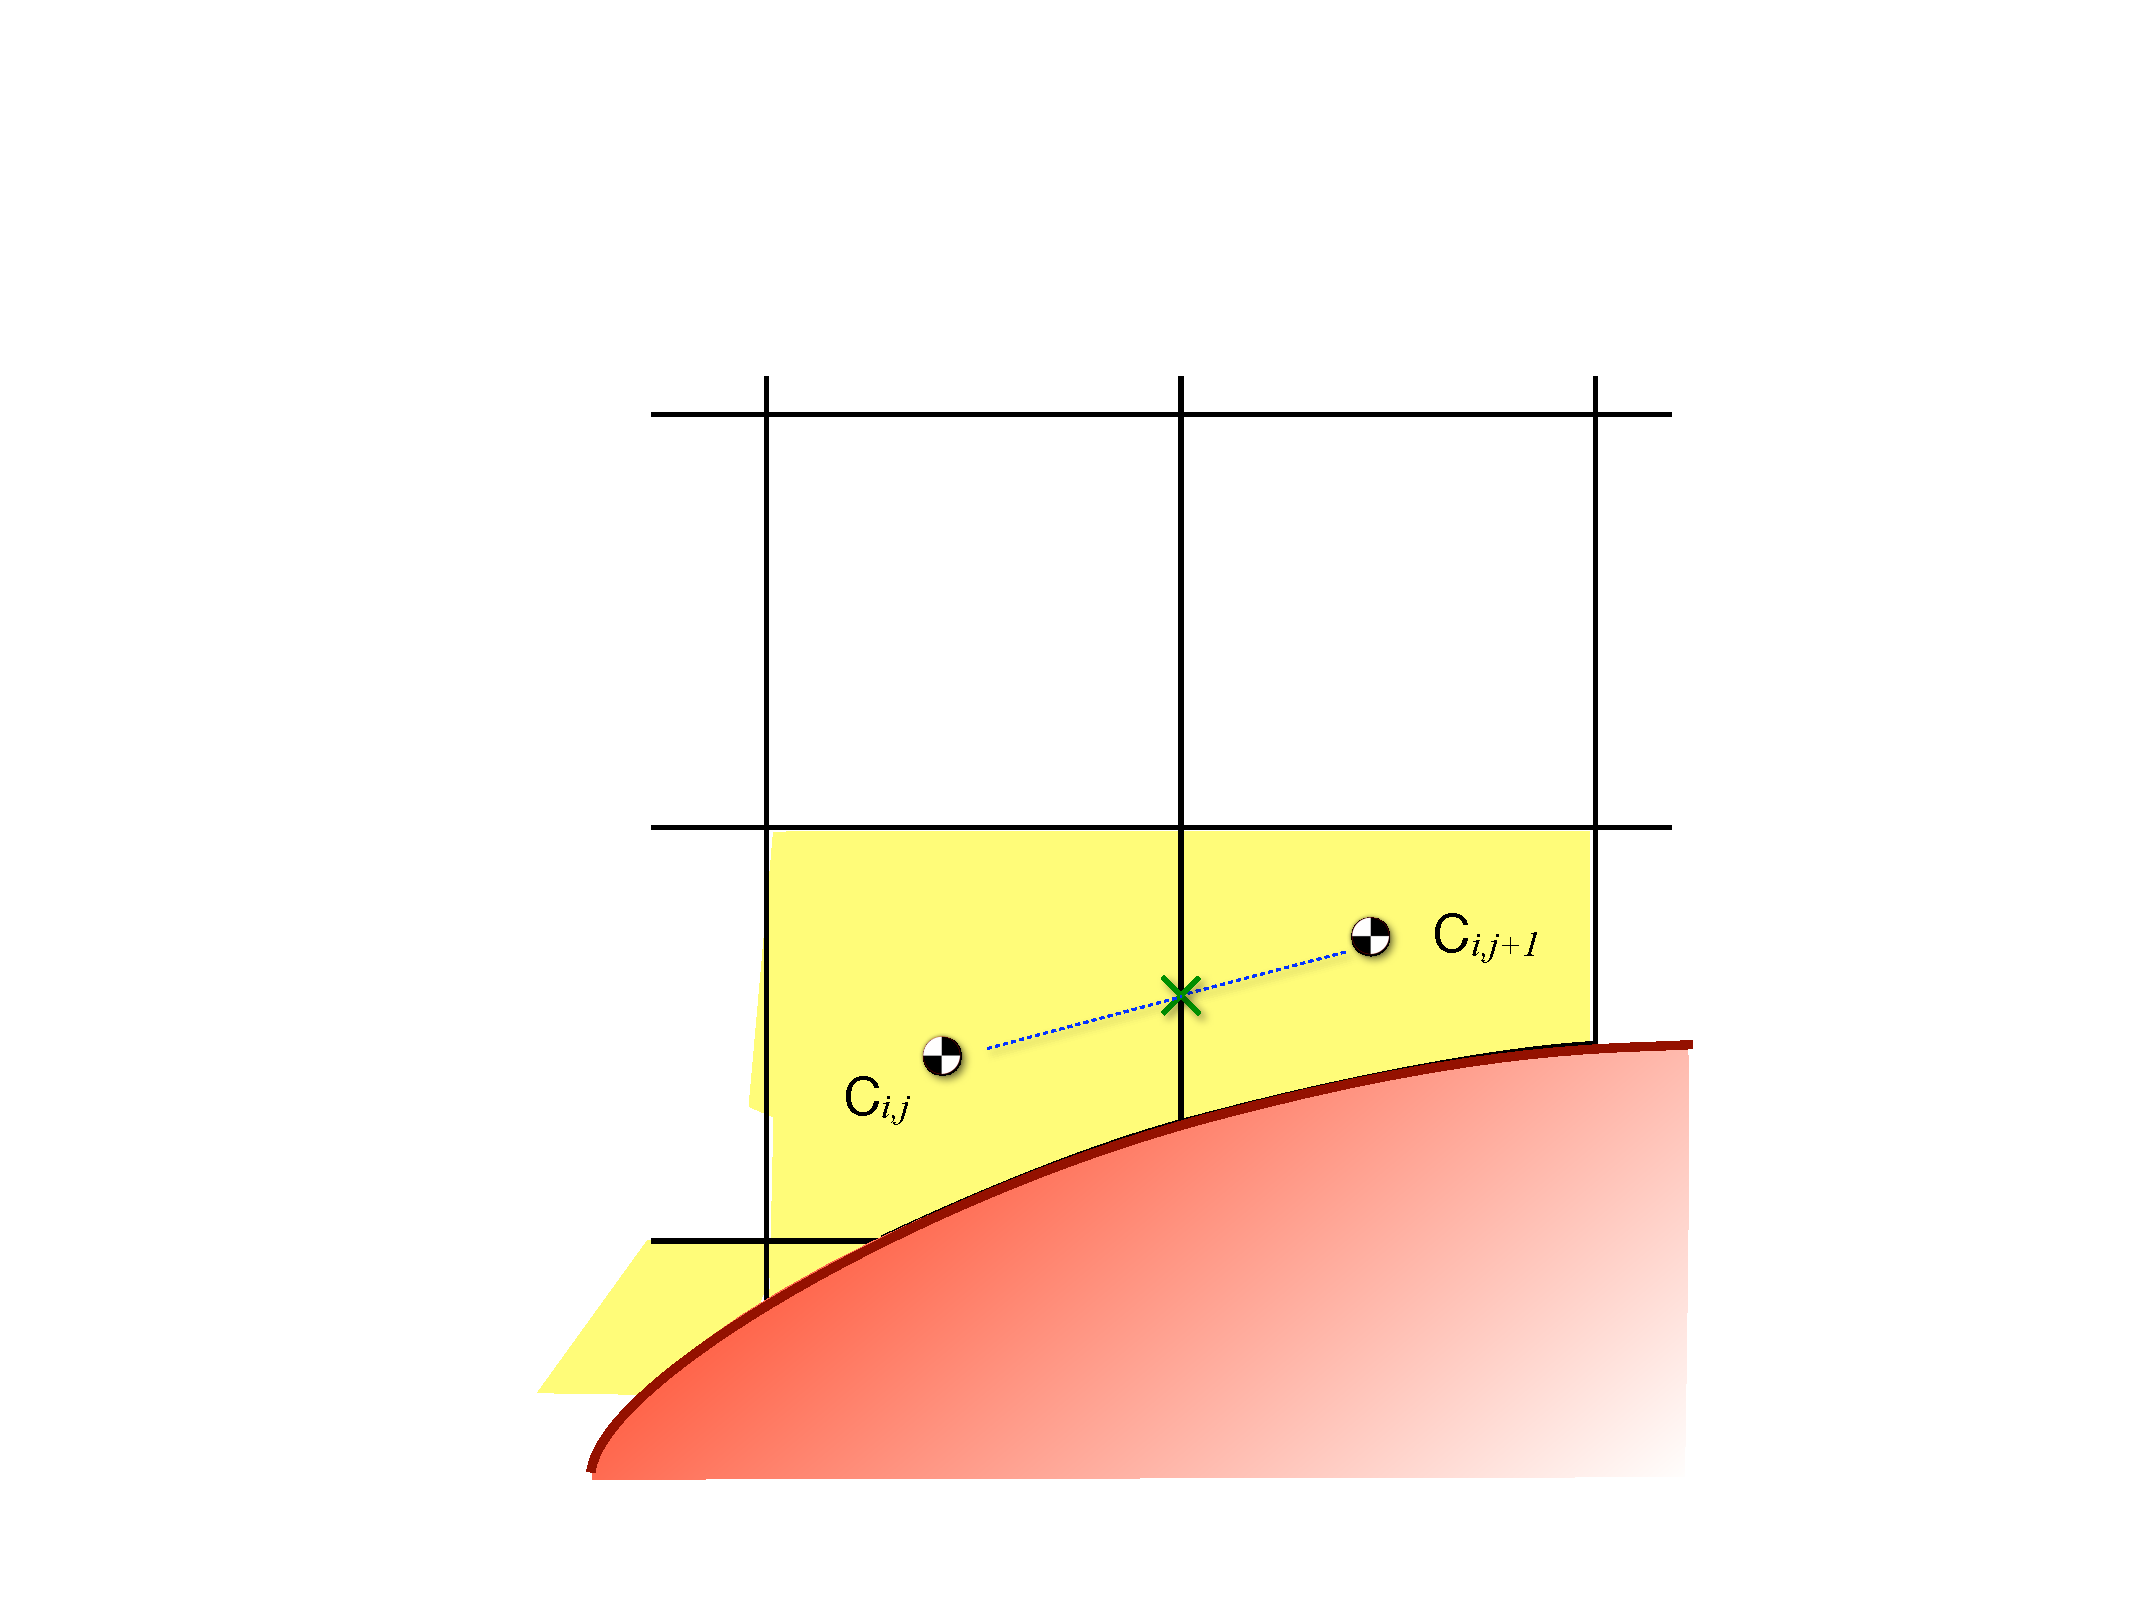
\includegraphics[width=3.2in]{figs/2dfig.pdf}
\caption{\sf Notation for mesh in two space dimensions. The cells shaded
in yellow are the cut cells.} 
\label{fig:2dfig}
\end{center}
\end{figure}

\subsection{Method of Lines approach}
The simplest scheme is to use a spatial discretization over the entire
mesh, and apply a Runge-Kutta scheme in time. This is a well-known
standard approach
on regular Cartesian meshes. It is adapted for the cut cells by
using a least squares reconstruction of the gradient that includes
either edge and node neighbors (the examples will always specify).
Limiting is done using the Barth-Jespersen limiter \cite{} 
on the cut cells and one adjacent neighbors. Any limiter
can be used for the regular cells.

The spatial reconstruction in the cut cells is no longer
coordinate-aligned, and need 
to include both $x$ and $y$ components of the gradient to 
reconstruct to the midpoint of the cell edge. This is indicated 
Figure \ref{fig:2dfig}  indicates this face location with a green $\times$.
The SRD stabilization scheme is applied after each stage of
the Runge-Kutta scheme. 
Note that the time step restriction that results from the von Neumann stability analysis of this scheme applied to the linear advection equation is  (AG -
TRUE or this is for positivity?)
\begin{equation}
\Delta t \,  \max\left(\frac{u}{\Delta x},\frac{v}{\Delta y}\right) \leq \frac{1}{2} ,
\end{equation}
where $(u,v)$ is the propagation velocity.  

\subsection{MUSCL scheme}
The MUSCL scheme is a one step method that is second order accurate in
time. The series of MUSCL schemes  was originated by van Leer 
\cite{vanleer:muscl}. The version\footnote{Thanks to Phil 
Colella for the original Cartesian mesh code as well}
we use is due to Colella \cite{Colella:Unsplit}.
The method is briefly sketched here so that we can describe how it
was adapted for cut cells.

On a regular cell $(i,j)$ the interface values on the surrounding
faces are computed at the half-step in time and passed to a Riemann
solver to compute the surrounding fluxes.
Using a Taylor series in space and time to second order around the
cell center, and using the equation to replace the derivative in time,  gives
\begin{equation}\label{taylor}
\begin{split}
q_{i+1/2,j}^{n+1/2} & = q_{i,j}^n + 
              \frac{\Delta t}{2} \frac{\partial q_{ij}^n}{\partial t} + 
              \frac{\Delta x}{2} \frac{\partial q_{ij}^n}{\partial x} \\[.1in]
            &  = q_{i,j}^n + \frac{\Delta t}{2} 
            (-\frac{\partial f_{ij}^n}{\partial x} -
             \frac{\partial g_{ij}^n}{\partial y})  +
             \frac{\Delta x}{2} \, \frac{\partial q_{ij}^n}{\partial x} \\[.1in]
            &  = q_{i,j}^n - \frac{\Delta t}{2} \, 
             \frac{\partial g_{ij}^n}{\partial y}  -
            ( \frac{\Delta t}{2} 
            \frac{\partial f_{ij}^n}{\partial q} -
             \frac{\Delta x}{2} ) \,\frac{\partial q_{ij}^n}{\partial x} \\[.1in]
\end{split}
\end{equation}

At regular cells, the term $\partial g / \partial y$ is computed by solving Riemann
problems in the $y$ direction,  evaluating the flux $g$, and computing the
difference in the $y$ direction.
Since this only needs to be done to first order accuracy (the term is multiplied
by $\Delta t$)  no reconstruction to in the transverse direction was necessary,
and differencing the edge fluxes is appropriately cell-centered.
(For other details the reader is referred to \cite{Colella:Unsplit}.)
Furthermore, it is the transverse derivatives that provide corner coupling,
giving the MUSCL scheme at stability limit of
\begin{equation}
\label{eqn:bigcfllimit}
\Delta t \, \max \left (\frac{u+c}{\Delta x} , \frac{v+c}{\Delta y} \right) < 1
\end{equation}

At the cut cells we can no longer do this.  We made two modifications. First,
the solution is reconstructed to the edge midpoint  for the transverse Riemann problem.
This takes care of the situation where a full cell is adjacent to a cut cell, and
the transverse flux would not be centered. This is the situation
in \ref{fig:2dfig} for cell $(i,j-1)$, for example.
Secondly, most cut cells will not have a flux on the other side to form a
transverse derivative, for example cell $(i+1,j)$. Even for cell $(i,j)$ is would
be difficult to find a location where the vertical fluxes could be differenced.
For these cut cells, the transverse derivative term is handled by instead computing
$ \partial G / \ \partial y \, = \,  \partial G / \partial q \times \partial q / \partial y$,
as with the horizontal fluxes.

The transverse derivatives are necessary to keep the method linearly exact in the
cut cells. 
However, in the neighborhood of a shock the derivatives will be limited, and
possibly set to zero.
Without these terms in the volume  the time step would be reduced to 
\begin{equation}
\Delta t \, \left (\frac{u+c}{\Delta x} + \frac{v+c}{\Delta y} \right) < 1
\end{equation}
which could be as small as half the larger limit \eqref{eqn:bigcfllimit}.
However, as shown in \cite{mjb:stability2} for one space dimension, 
boundary cells can have
a local {\em cfl} number that is up to twice the stable {\em cfl} of the regular
mesh and the overall scheme remains stable.  We have not found any stability
problems due to this term.  

Finally, we use the LP-limiter \cite{May_Berger_LP} for the cut 
cells and one adjacent, to try
to retain as much of the gradient as possible. The cells two away from a cut cell
can use any limiter. In the computational examples that use the MUSCL scheme, 
monotonicized central differencing, also known as van Leer limiting,  
is used on the regular cells.



\section{The State Redistribution Algorithm}\label{sec:srdAlg}

We first describe the second order accurate version of the State
Redistribution Algorithm. 
This helps simplify the notation and make the
algorithm more intuitive.   
At several places there are choices
to make, and we discuss the alternatives and the reason behind our
choices.  

\subsection{The State Redistribution Algorithm}

To start, we define two quantities associated with each cell of the mesh:

\begin{itemize}
\item
{\bf Each cut cell finds adjacent cells to {\em temporarily} merge with.}

\vspace*{.1in}
For each cut cell in the mesh, find  one or more neighbors until the
volume of the temporarily merged cell is at least half the area of an uncut cell, i.e., 
\begin{equation} \label{eq:vmerge}
\sum_{(k,l) \in M_{i,j}} V_{k,l} \geq \frac{1}{2}\Delta x\Delta y,
\end{equation}
where $M_{i,j}$ denotes the set of cell indices that belong to merging neighborhood $(i,j)$.
We call this the 
{\em  merging neighborhood} or {\em merging tile}.  
A small cell can be merged with cells in the direction closest to the boundary normal (Figure \ref{fig:neighborhoods}, left), or with all cells that are at most e.g. one cell away, that is, cells located on the $3 \times 3$ tile centered at the small cell (Figure \ref{fig:neighborhoods}, right).
The larger the neighborhood the more diffusive the results, therefore we use the normal neighborhood everywhere possible.
There are instances where the normal neighborhood cannot be used, e.g., if a neighboring cell is also cut and the
merging neighborhood is not sufficiently large (Figure \ref{fig:normalneighborhood}).  In this case, we must merge with cells on the $3\times3$ tile (Figure \ref{fig:3x3neighborhood}), or, if that merging neighborhood is not large enough, with cells on the $5 \times 5$ tile.

\begin{figure}
    \centering
    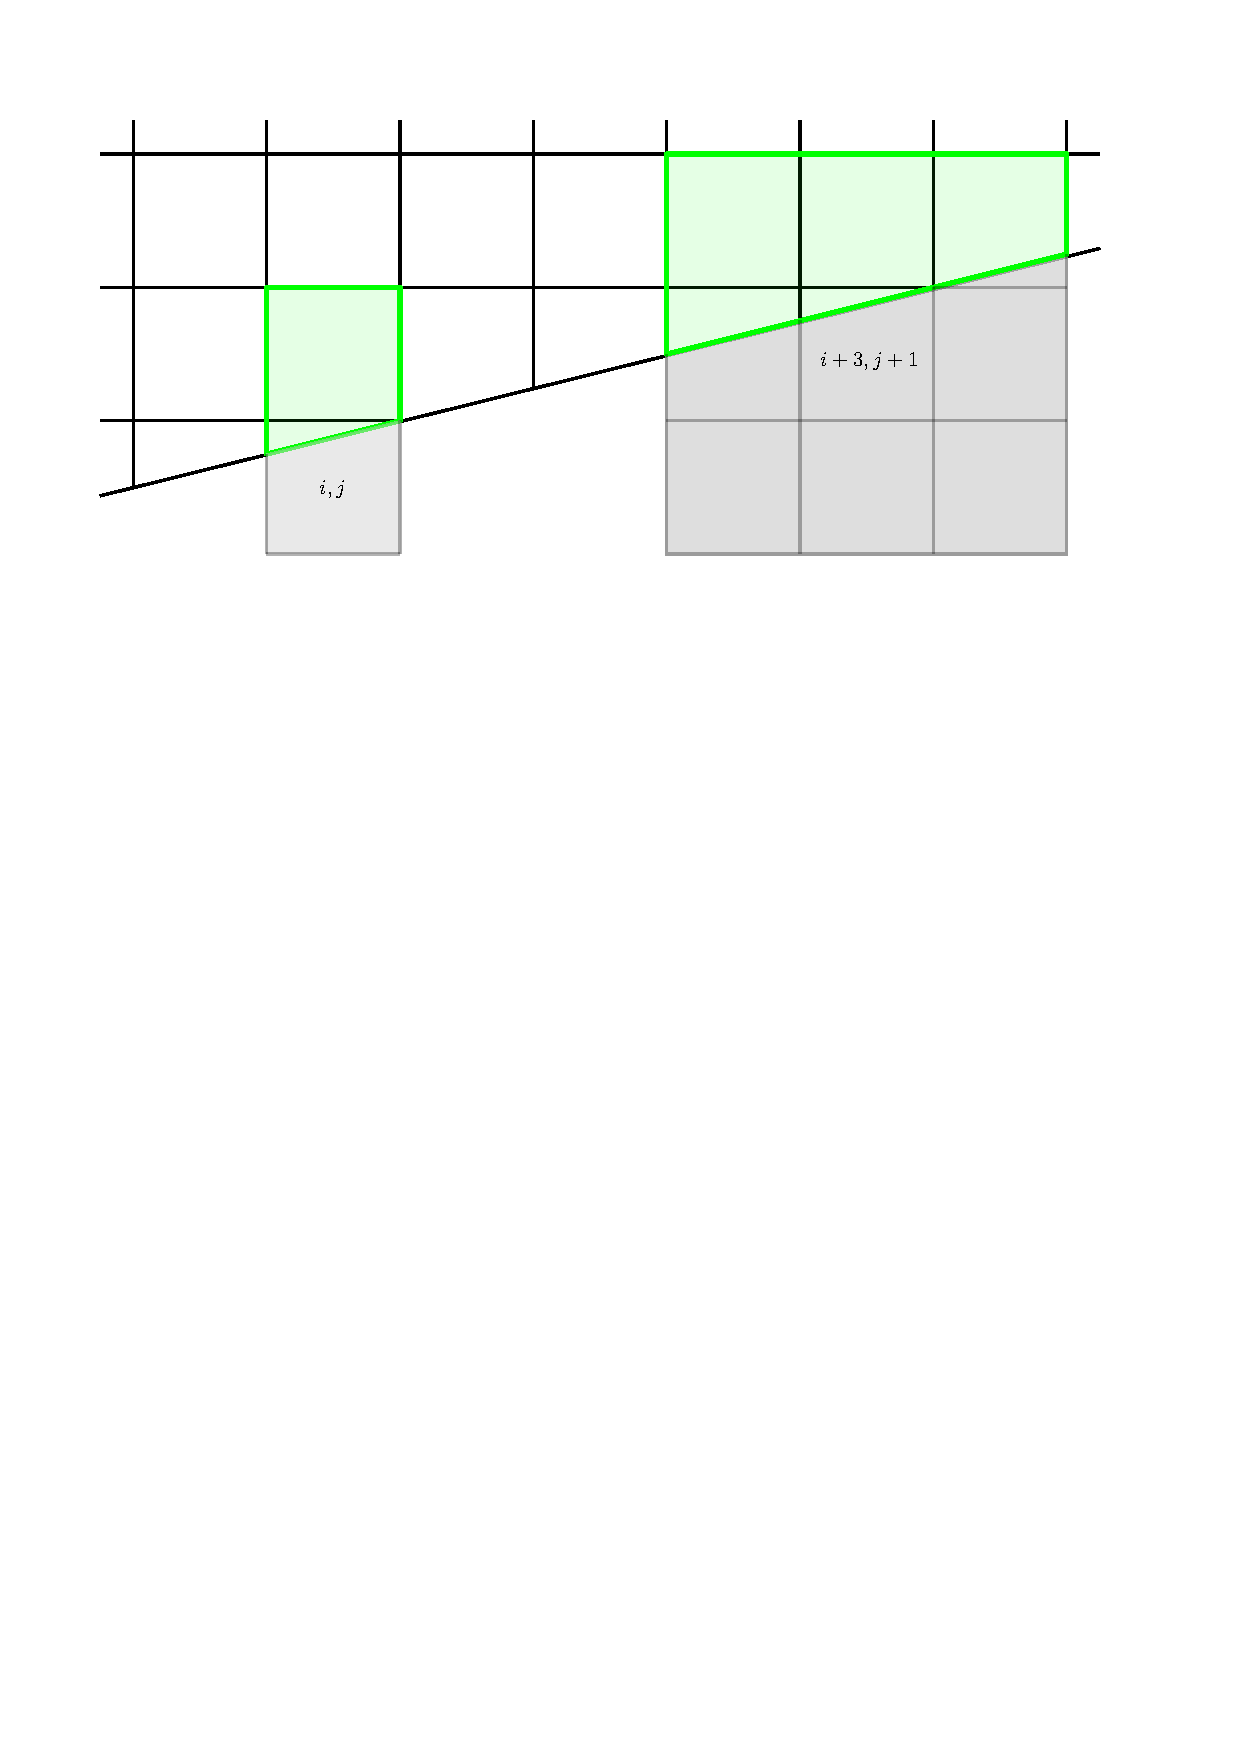
\includegraphics[width=0.5\linewidth]{figs/neighborhoods.pdf}
    \caption{\sf On the left, a small cell is merged with a cell in the direction 
    normal to  the wall.  On the right, a small cell is merged with neighbors that are at most one cell away, i.e., cells located in the $3\times3$ tile.}
    \label{fig:neighborhoods}
\end{figure}

\begin{figure}
	\subfloat[\sf Normal neighborhood (in red) for both small cells in the right corner.]{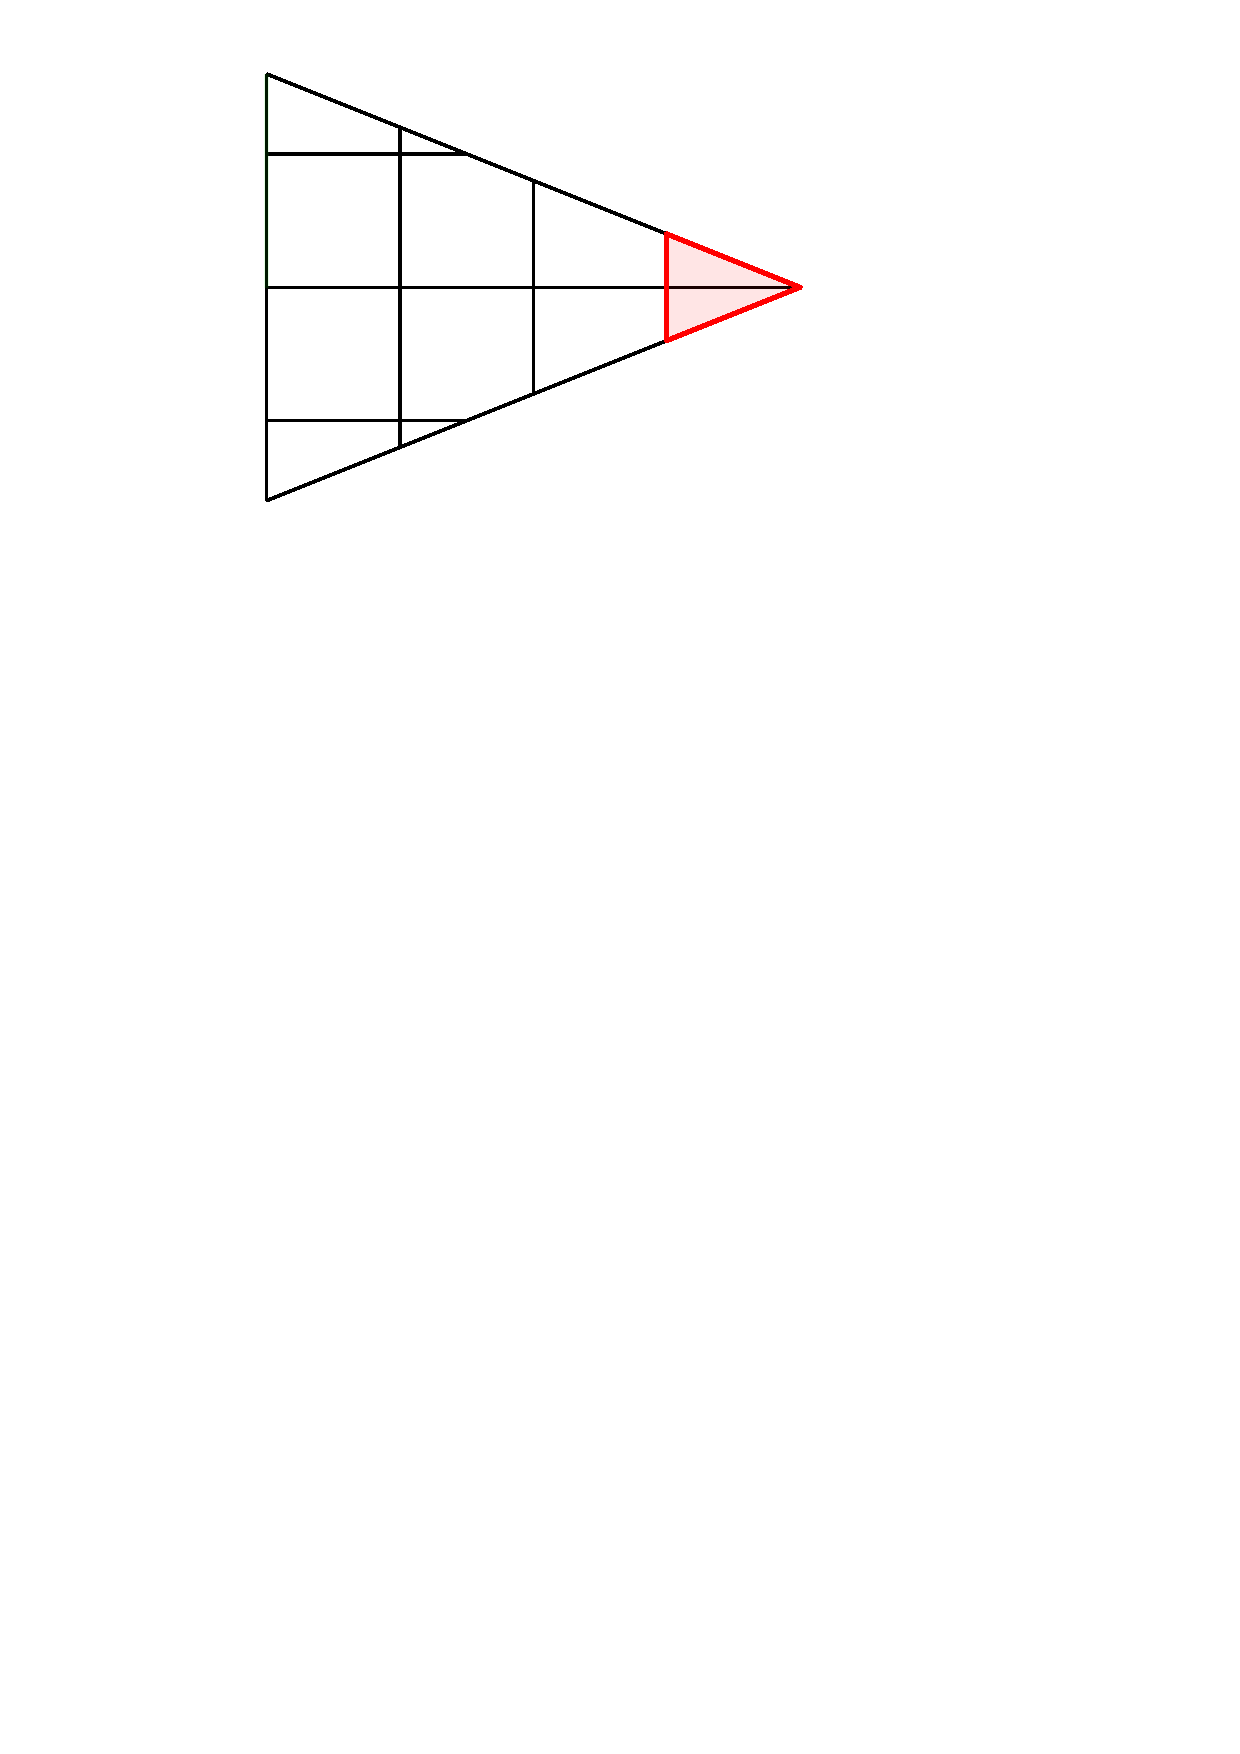
\includegraphics[width=.45\textwidth]{figs/normaldirection1.pdf} \label{fig:normalneighborhood}}
	\hfill
	\subfloat[$3\times 3$ merging neighborhood for both small cells in the right corner.]{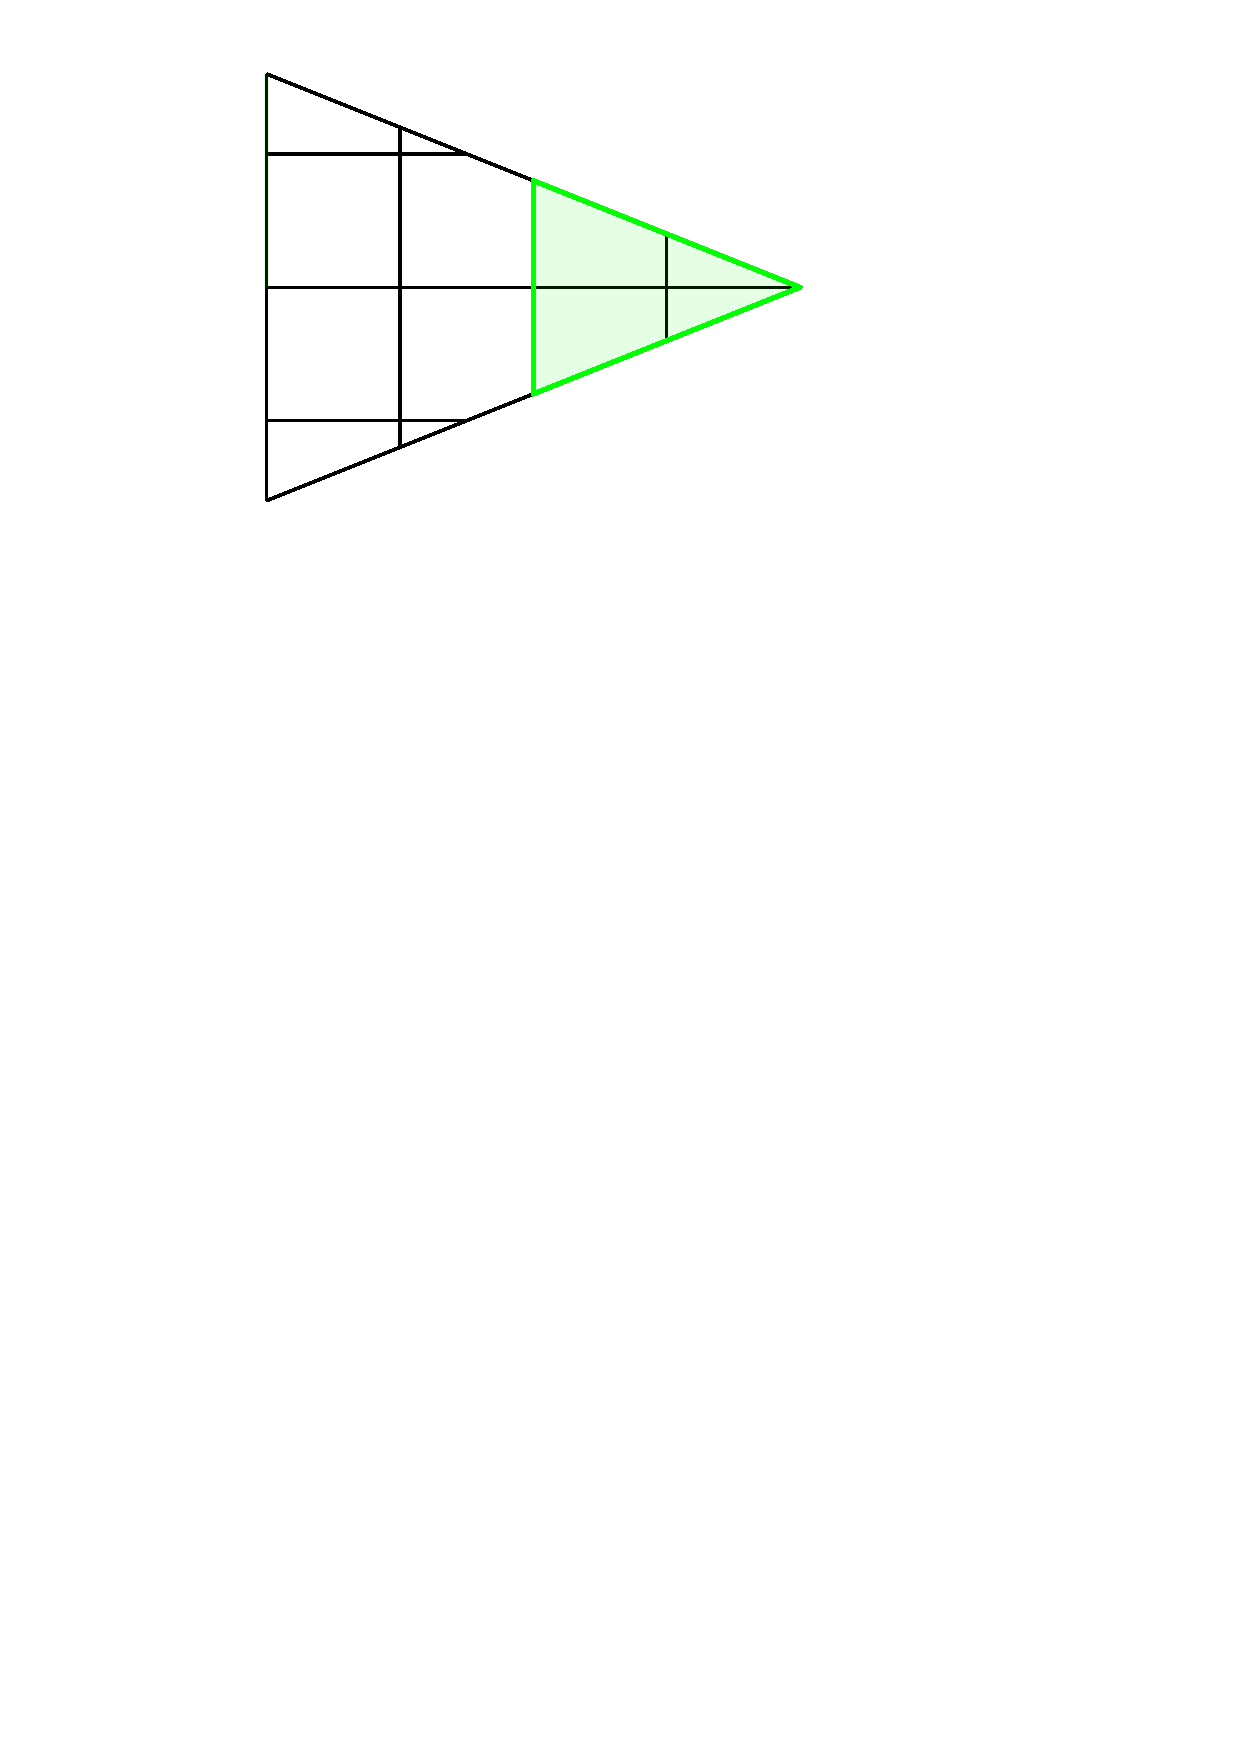
\includegraphics[width=.45\textwidth]{figs/normaldirection2.pdf} \label{fig:3x3neighborhood}}
	\caption{\sf Sometimes, the normal neighborhood is not large enough if a small cell merges with another small cell.  In this case, we use the $3\times 3$ tile, or $5\times5$ neighborhood until the volume constraint \eqref{eq:vmerge} is satisfied.}
\end{figure}
% If the neighboring cell 
% is also cut, it can happen that the
% merged cell is not sufficiently large (SHOW EXAMPLE?). 
% Next we try a 2 by 2
% neighborhood, including the original cut cell. Later we also show
% results using a 3 by 3 neighborhoods. However the larger the
% neighborhood the more diffusive the results.

% Note that this does not have the difficulty of cell merging, since 
% overlapping neighborhoods are allowed. 

\item
{\bf Each cell counts how many neighborhoods it is a part of.}

\vspace*{.1in}
A full cell is its own merging neighborhood, since it has sufficient
volume all by itself. However, we will still refer to all cells as having a
merging neighborhood for ease of presentation.  In figure \ref{fig:overlappingneighs}, we provide an example cut cell mesh with all merging neighborhoods plotted.  We also display the number of overlapping neighborhoods on a cell, this is the neighborhood {\em count} for each cell.
\begin{figure}
	\subfloat[]{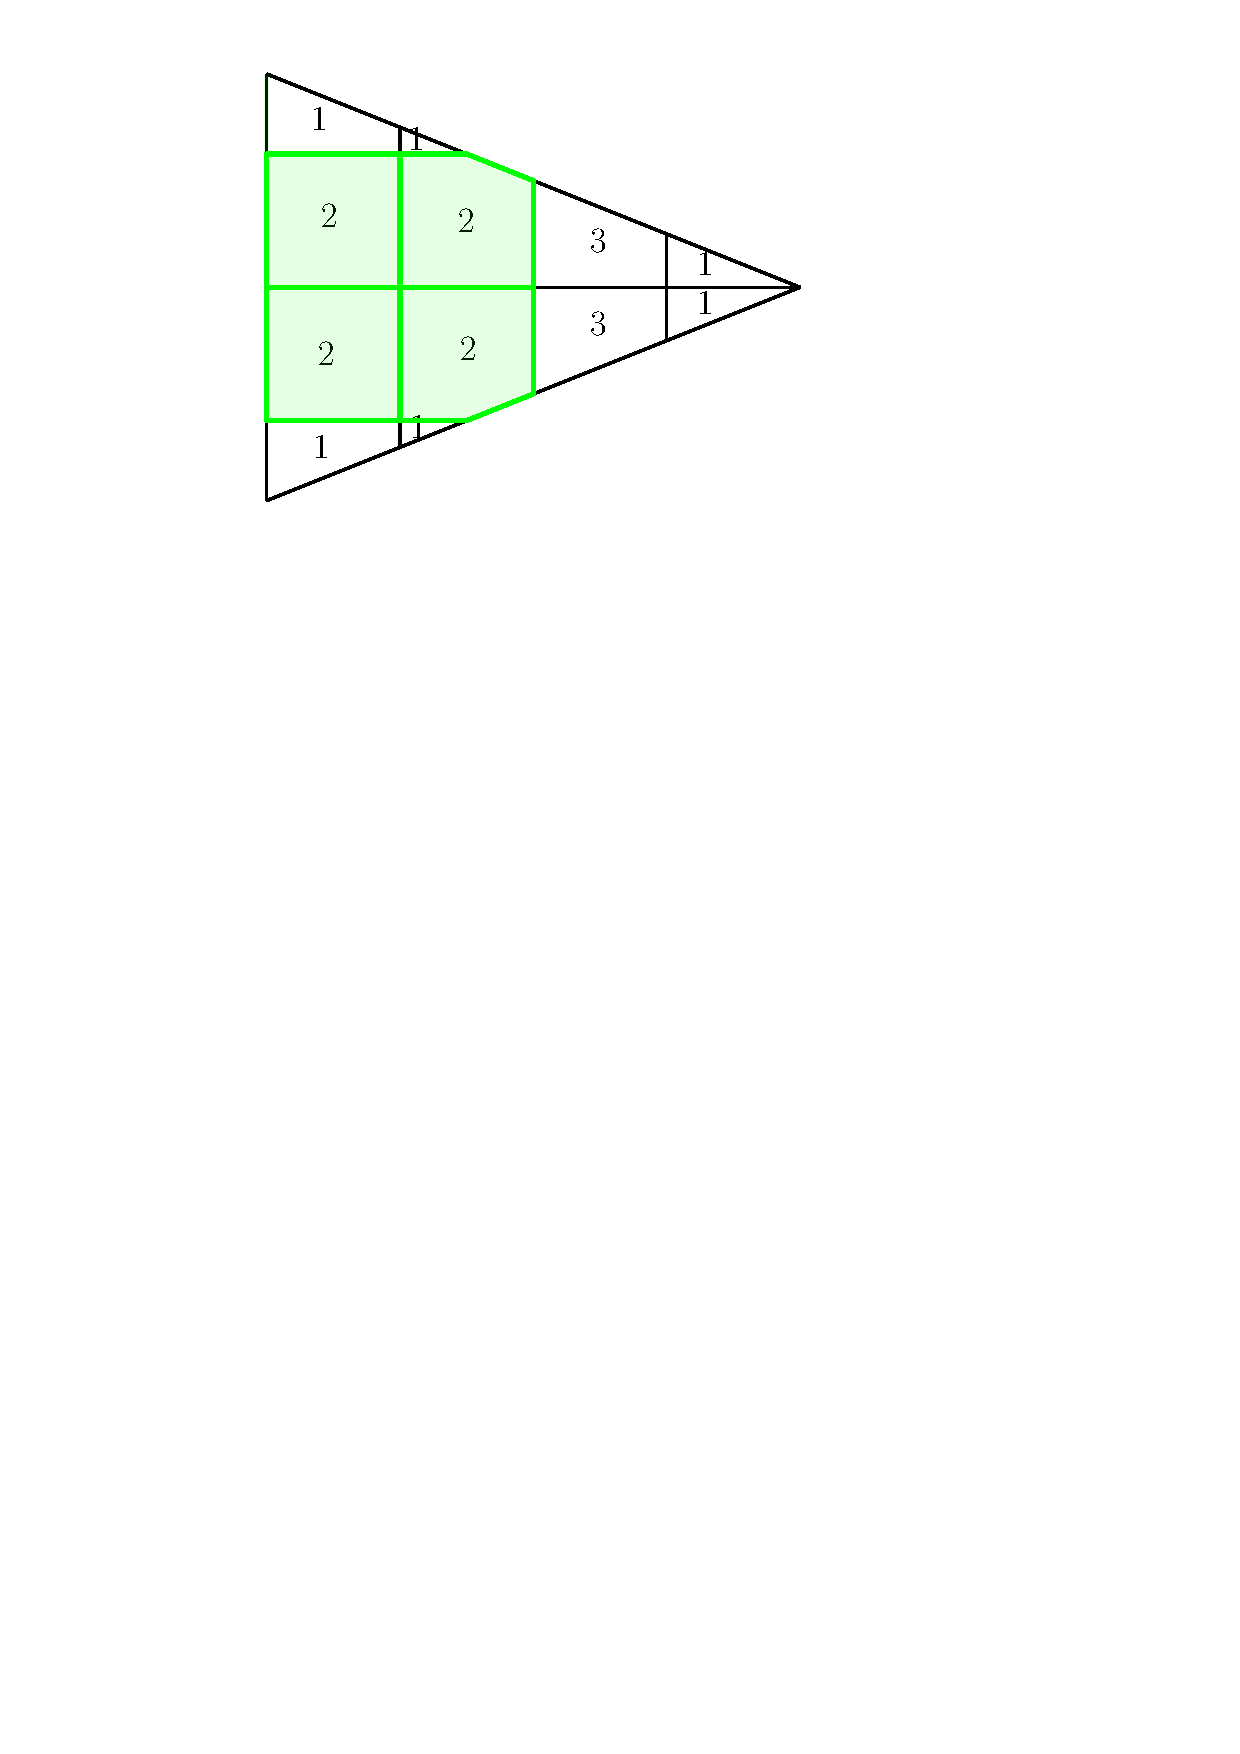
\includegraphics[width=.24\textwidth]{figs/numoverlaps1.pdf} \label{fig:numoverlaps1}}
	\hfill
	\subfloat[]{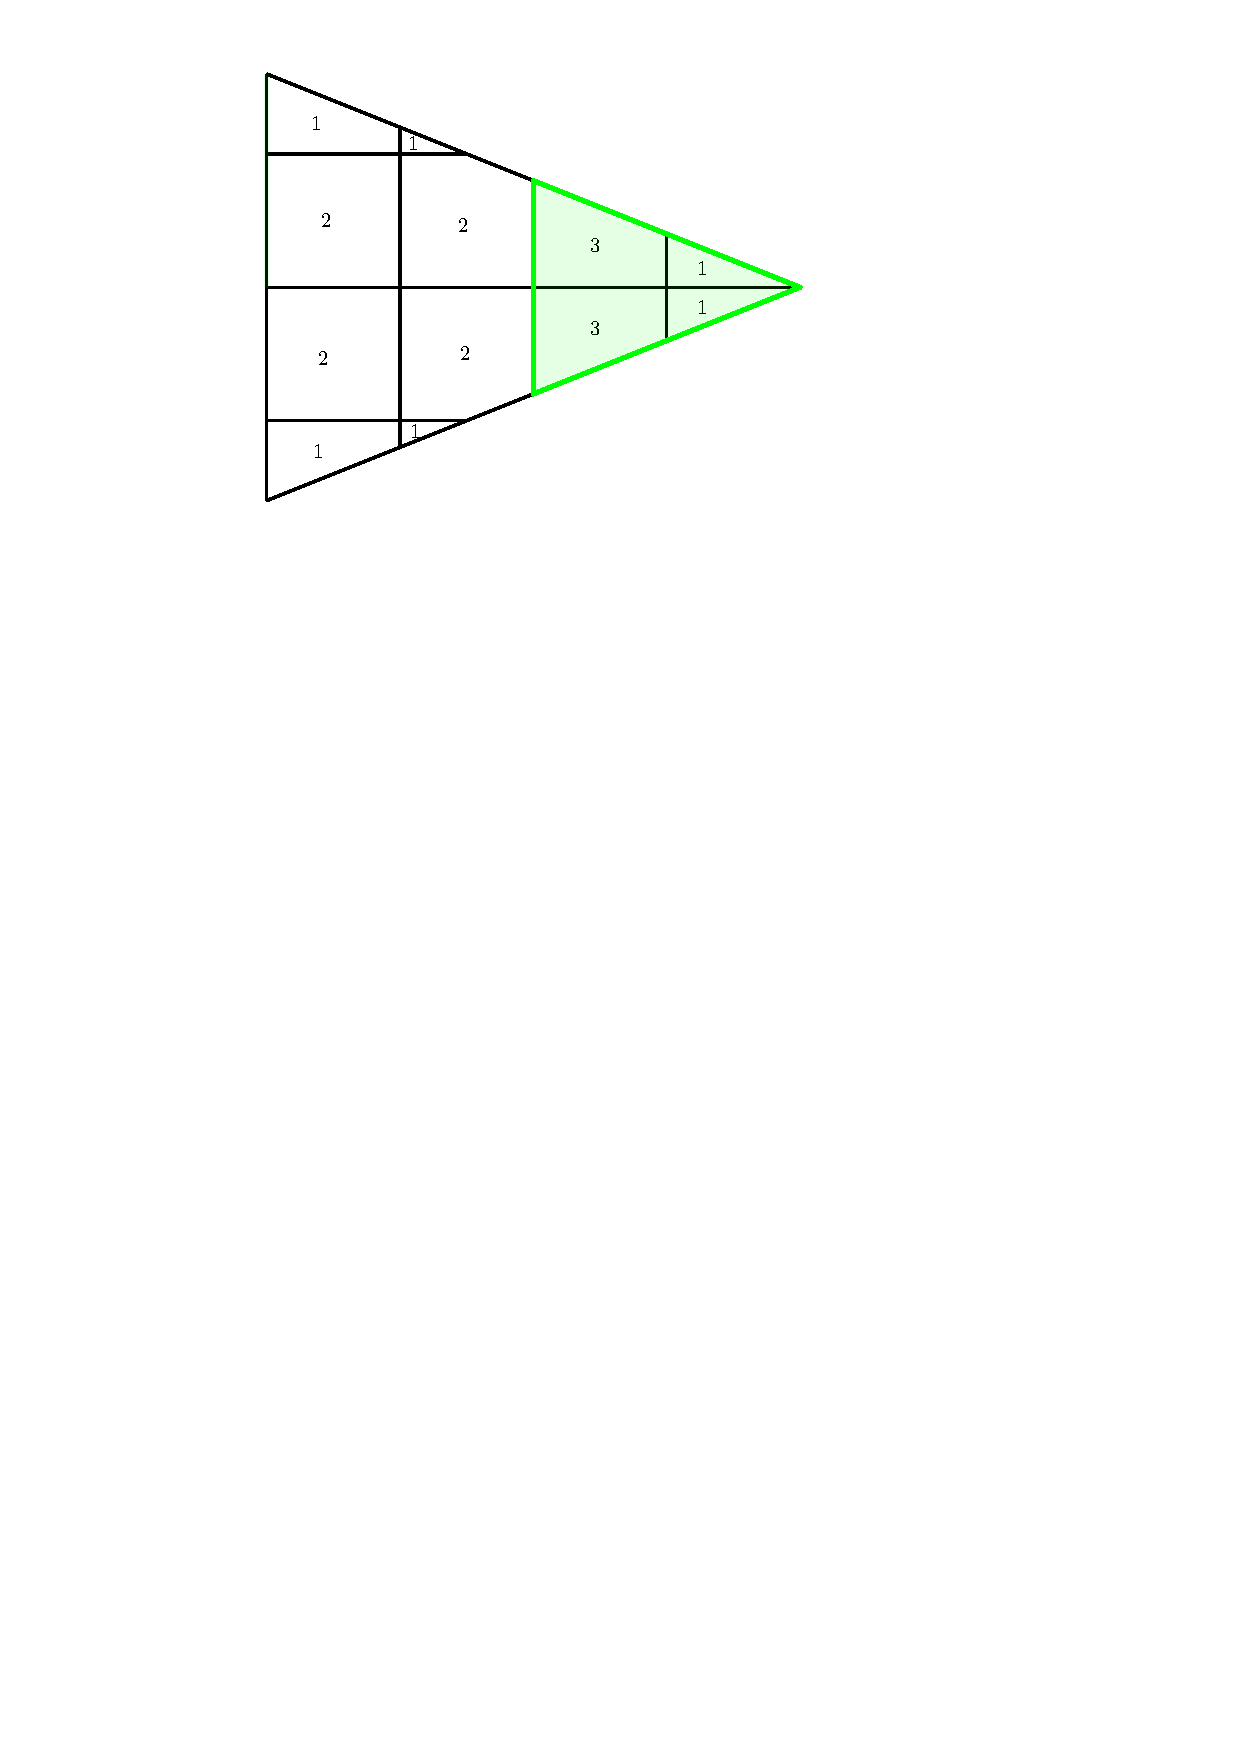
\includegraphics[width=.24\textwidth]{figs/numoverlaps5.pdf} \label{fig:numoverlaps4}}
	\hfill
	\subfloat[]{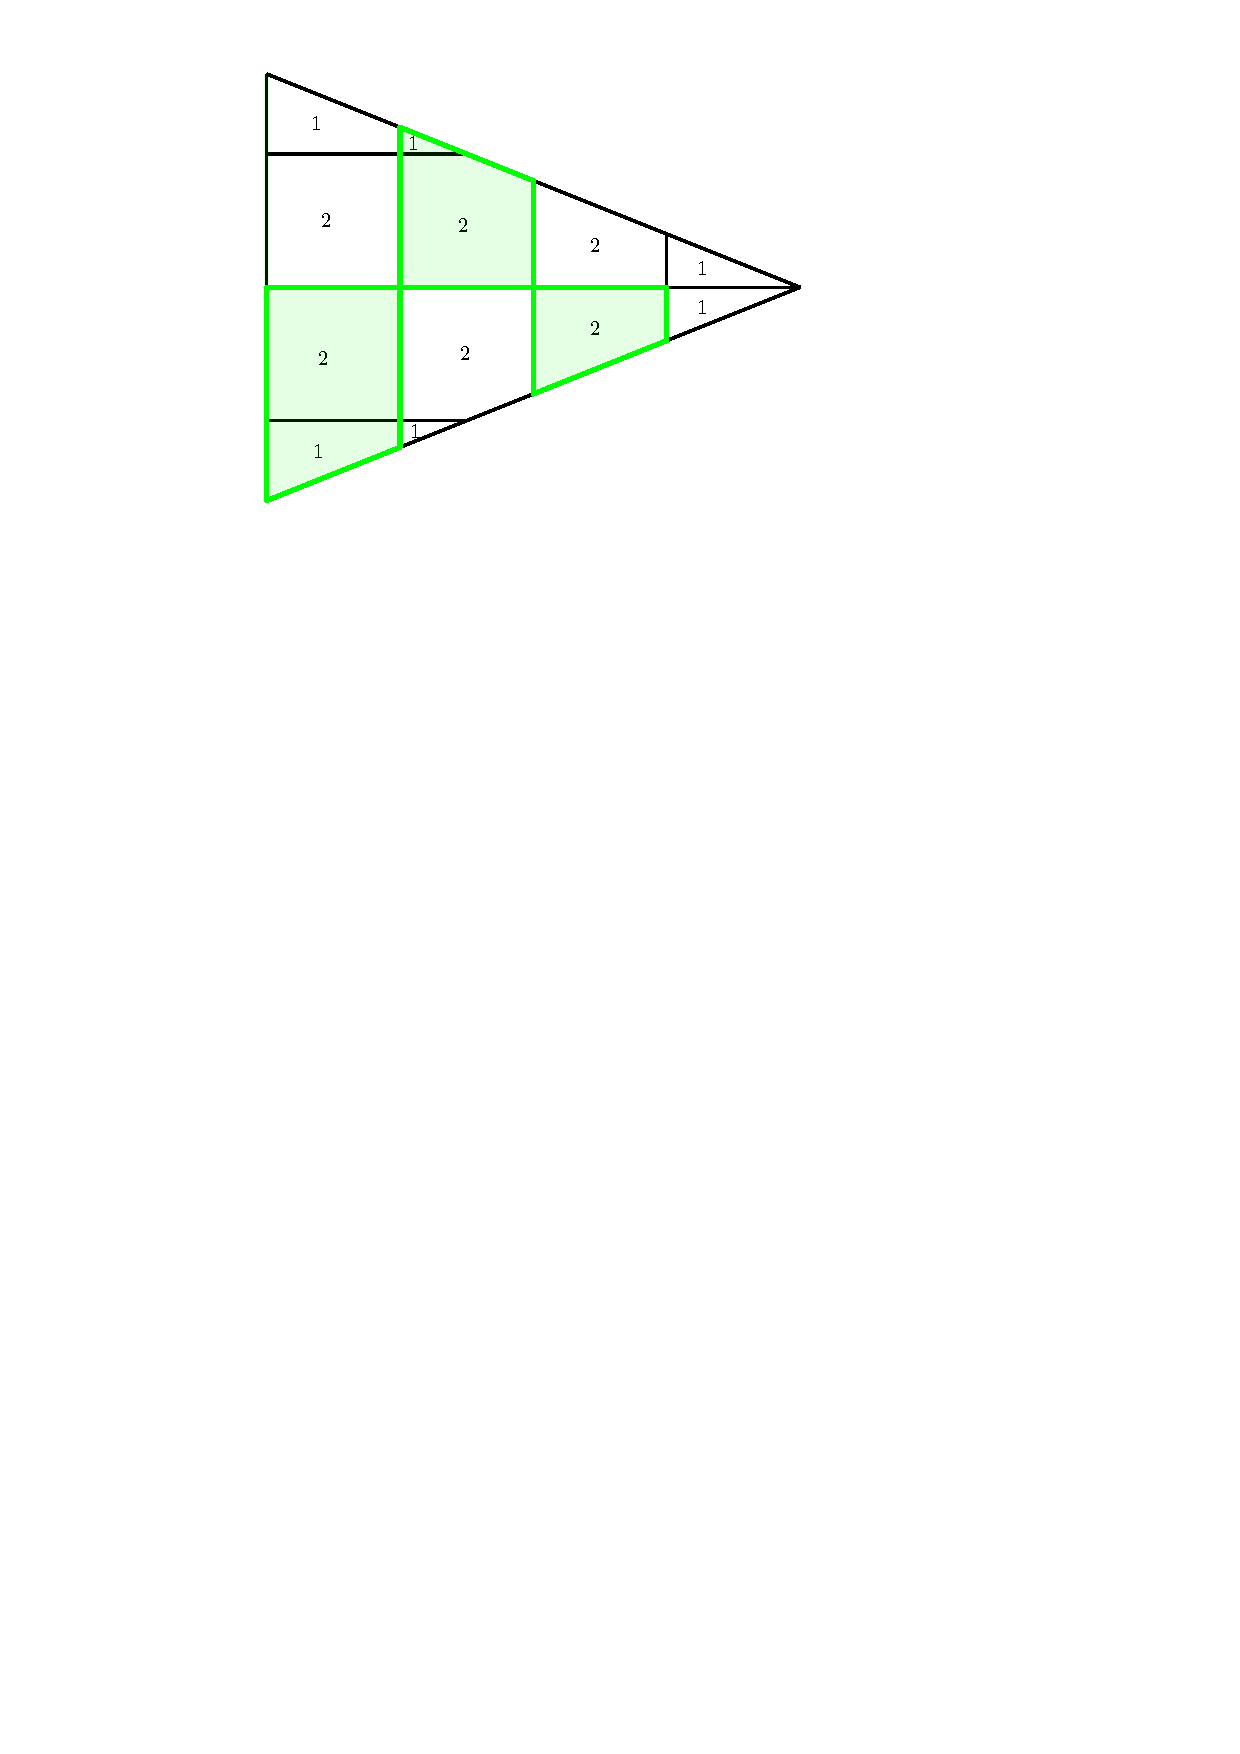
\includegraphics[width=.24\textwidth]{figs/numoverlaps2.pdf} \label{fig:numoverlaps2}}
    \hfill
	\subfloat[]{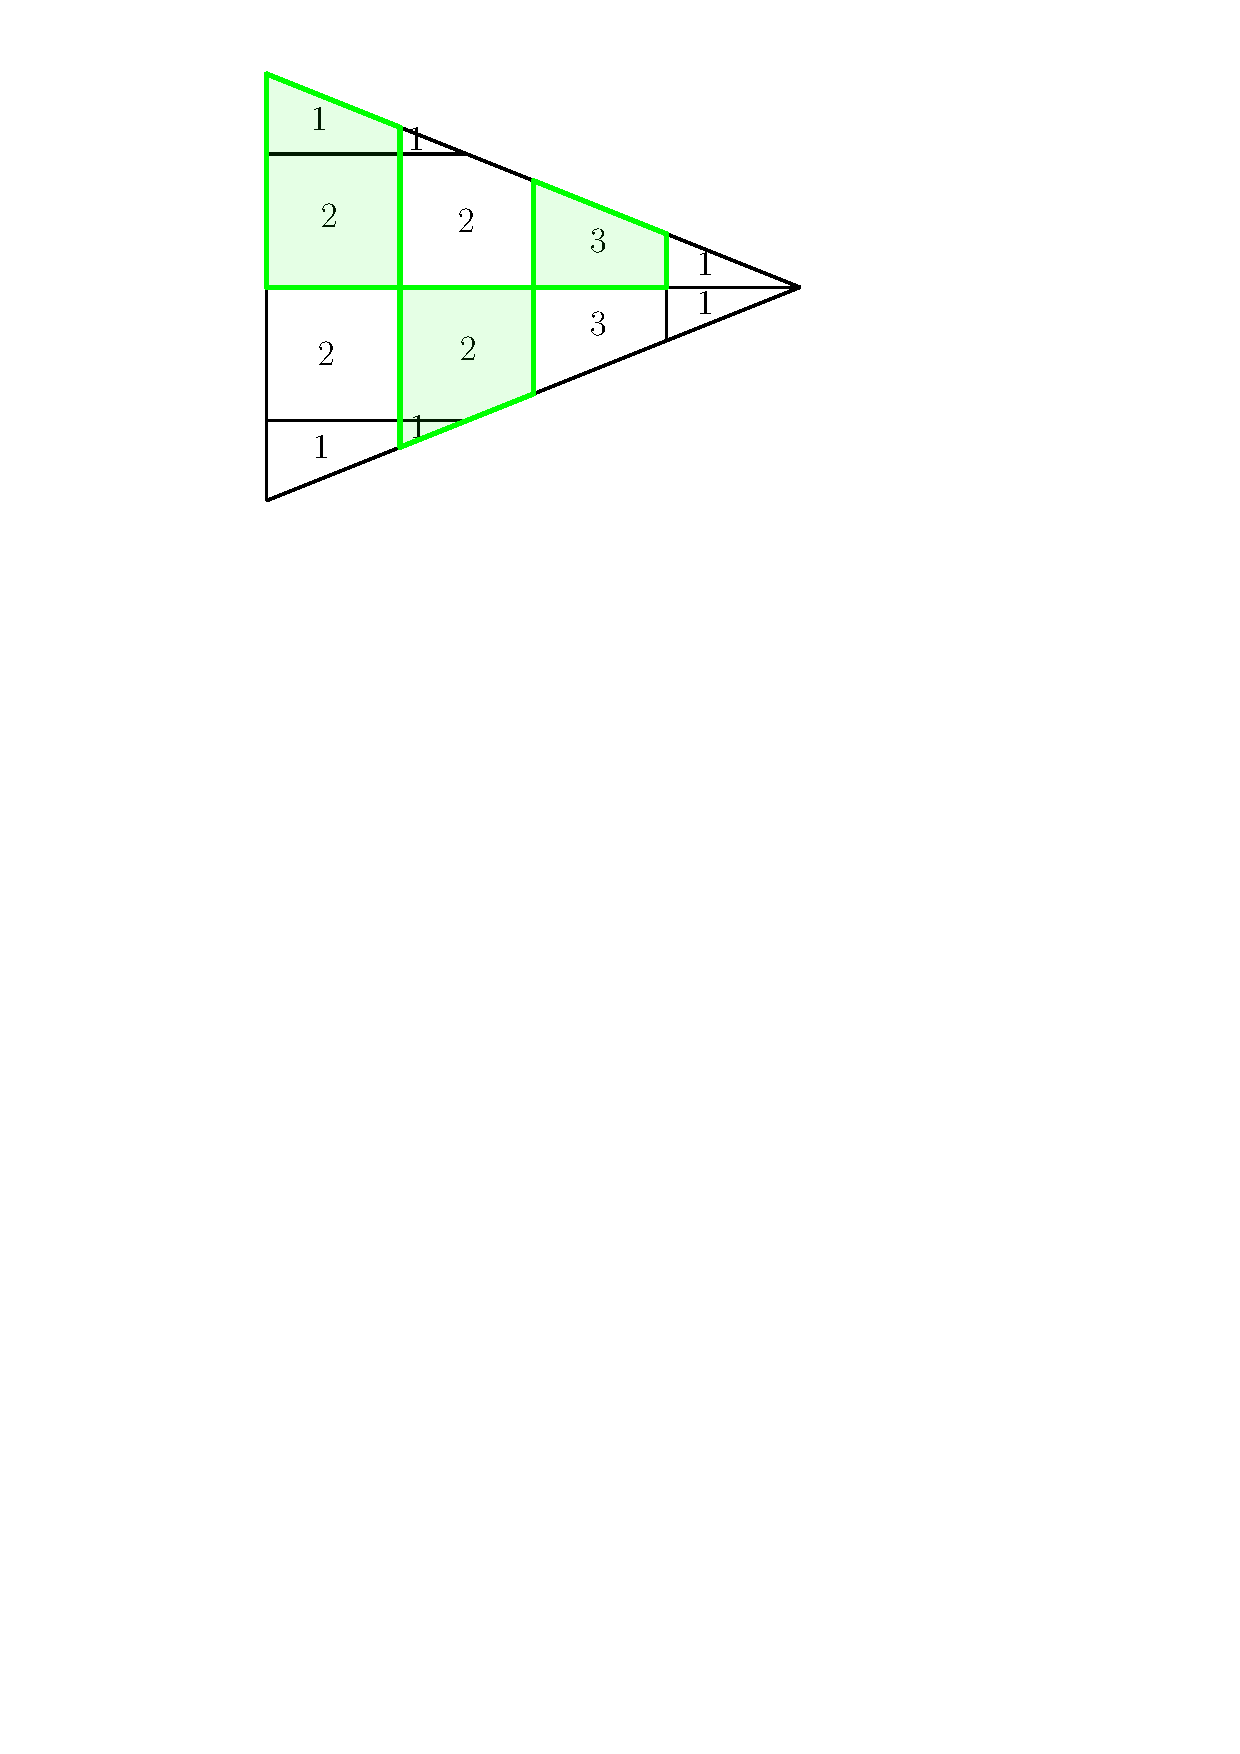
\includegraphics[width=.24\textwidth]{figs/numoverlaps3.pdf} \label{fig:numoverlaps3}}
	\caption{\sf All merging neighborhoods on an example cut cell mesh (in green).  We display the number of overlapping merging neighborhoods on each cell. Note, in figure \ref{fig:numoverlaps4}, there are two merging neighborhoods that occupy the same location, one per small cell in the right corner.} \label{fig:overlappingneighs}
\end{figure}
Note that a full cell
can be part of two or more merging tiles if it is placed next to 
several tiny cut cells. An example is shown in
figure \ref{fig:2nborTile}. The cells in green are part of two
neighborhoods, and those in red are part of three.   
 Most full
cells are only members of their own tile and will have a count of one.
Only cells within a narrow band of the cut cells will have a count
larger than one.


\end{itemize}



% \begin{figure}[h!]
% \begin{center}
% 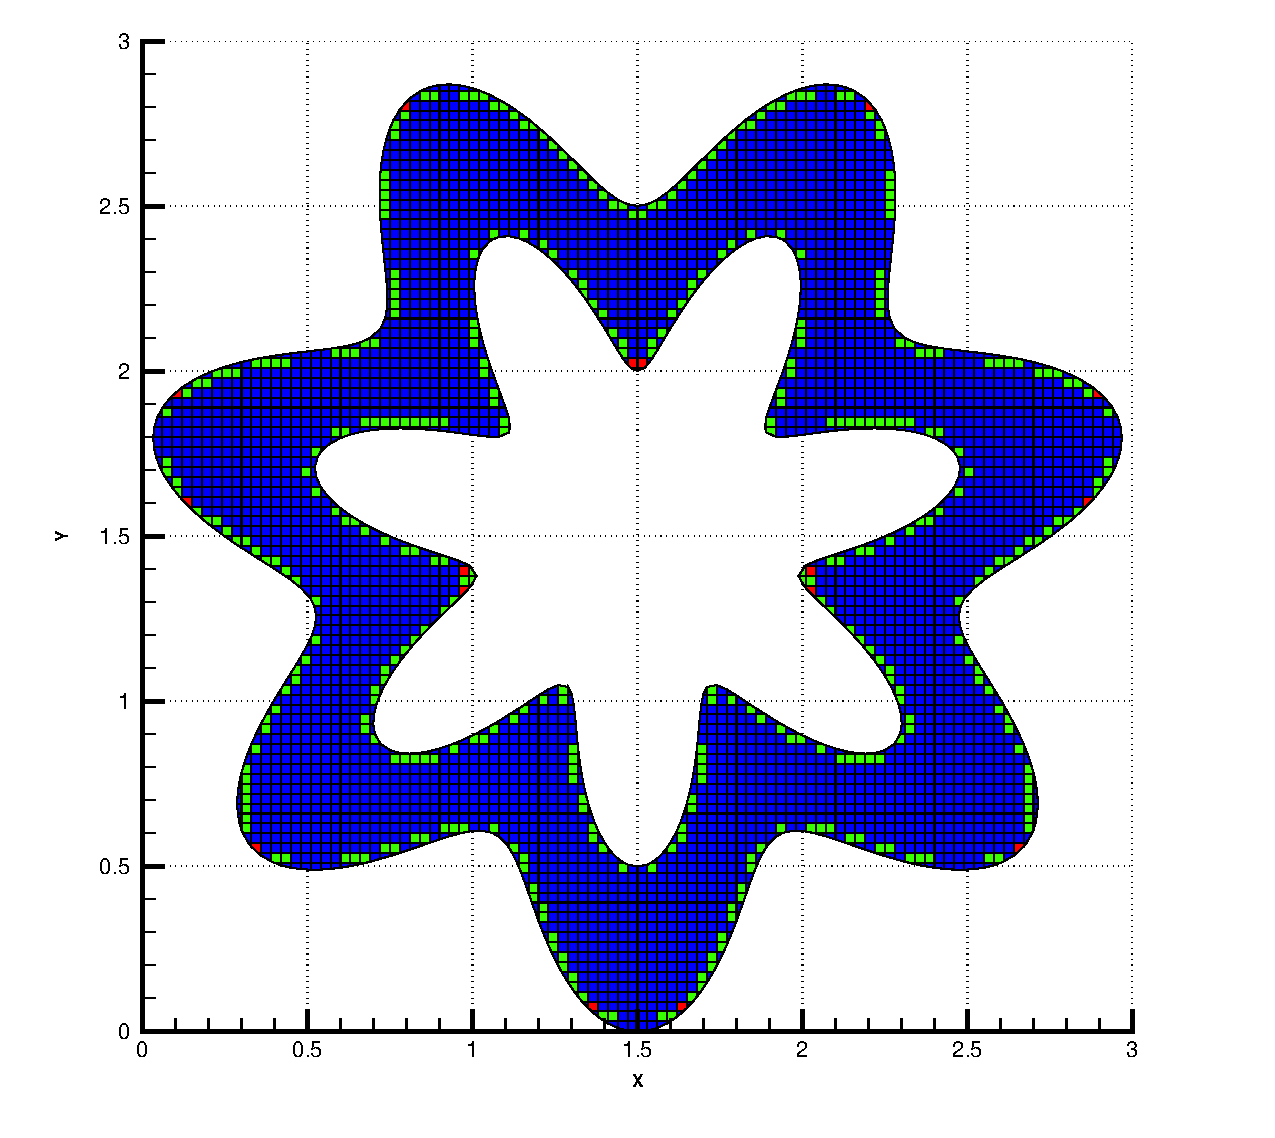
\includegraphics[width=4.5in]{figs/waveynumhoods.eps}
% \caption{\sf Domain from example XX.  Figure shows how many
% neighborhoods each cell belongs to: 
% one (white), two (blue), or three (red).
% The full example is shown in section \ref{sec:compResults}.}
% \label{fig:2nborTile}
% \end{center}
% \end{figure}

The two steps above can be part of a preprocessing step, since they do not
depend on the computed solution. For moving geometry however they would
be done at each step.
Using the merging tiles and the cell counts, the state redistribution
algorithm after one time step or stage is as follows:

%\begin{enumerate}[label=Step \arabic*:,leftmargin=2\parindent]
\begin{enumerate}
\item
{\bf Compute the volume-weighted and count-weighted solution for all
merged tiles.}   

\vspace*{.1in}
The contribution of each cell is divided by the number of neighborhoods 
it is part of (i.e. its count). The notation in this section refers
to cut cell $i,j$, with solution $U_{i,j}$ and volume
$V_{i,j}$. 
The provisionally updated solution before the
stabilization algorithm is applied is $\widehat{U}_{i,j}$.
There will now be many temporary merging neighborhoods which 
we denote as $\widehat{Q}_{i,j}$. 
Let $M_{i,j}$ denote the set of cell indices in the cell $(i,j)$ merging
neighborhood.  Then
\begin{equation}
\label{tiledef}
\widehat{Q}_{i,j} =  \frac{1}{{\widehat V}_{i,j}} \, \sum_{k \in M_i} \,  
\frac{V_k}{N_k}  \,\,  \widehat{U}_k
\end{equation}
where the volume ${\widehat V}_{i,j}$ is the merging tile volume similarly weighted,
\begin{equation}
\label{voldef}
{\widehat V}_{i,j} =  \sum_{k \in M_i } \,  \frac{V_k}{N_k}  .
\end{equation}

In other words, the contributions from each cell are weighted by the
number of neighborhoods they contribute to.
In the above equations, $k$ is  a multi-index ranging over the neighbors 
of cell $i,j$ included in its merging tile.
Note that most full cells will have ${\widehat V}_{i,j} = V_{i,j}$, 
and $\widehat{Q}_{i,j}  = \widehat{U}_{i,j}$.





\item
{\bf Compute a (limited) gradient for each merging
tile.}

\vspace*{.1in}
For cut cells, a least squares procedure  similar to the one used for
the finite volume update is an obvious choice. However instead of using the
solution $U_{i,j}$ on the Cartesian mesh at time $t_n$,
the merging neighborhood solution  $\widehat{Q}_{i,j}$ is used. It is important
to note that the centroid of the merging neighborhood is \textit{not} the centroid of cell ${i,j}$ (figure \ref{fig:centroids}).
\begin{figure}
    \centering
    \subfloat[]{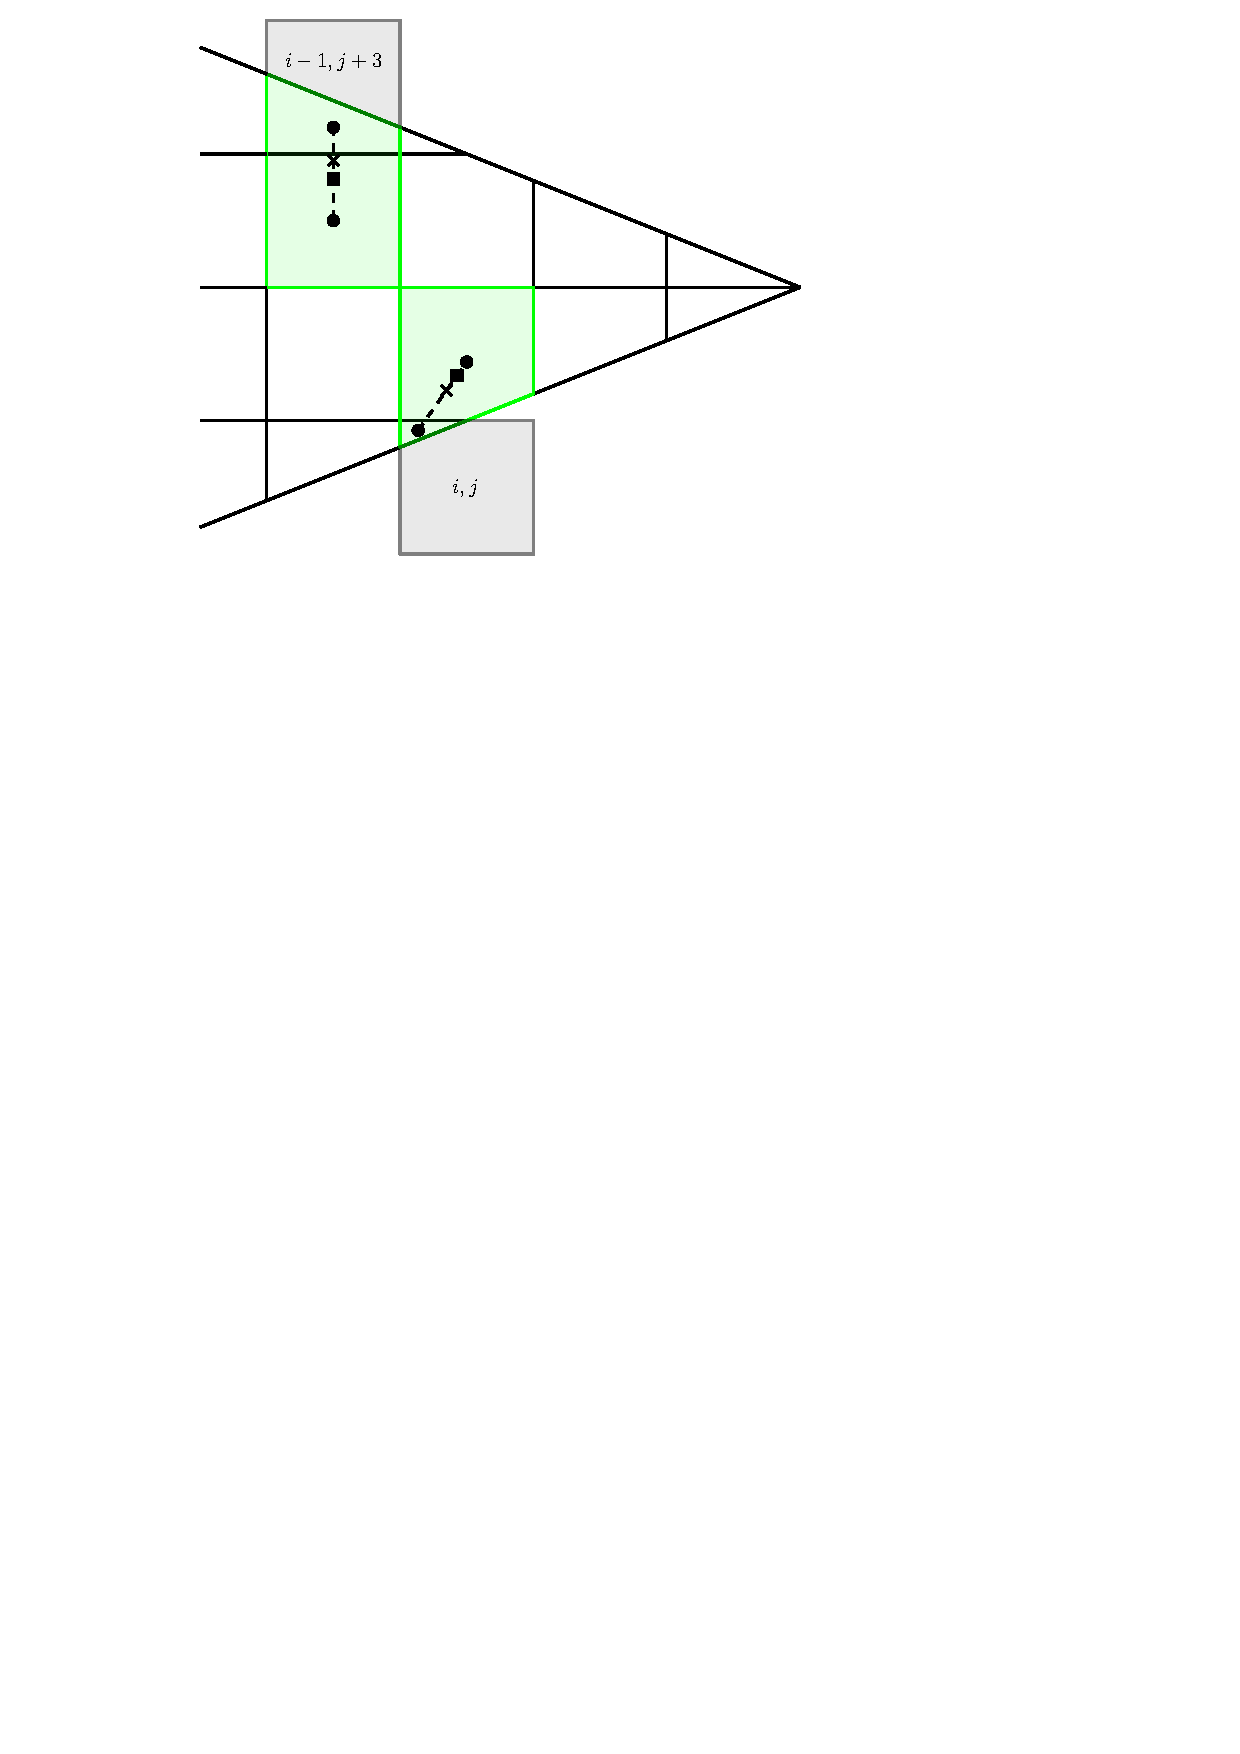
\includegraphics[width=0.45\linewidth]{figs/centroids3.pdf}} \hfill
    \subfloat[]{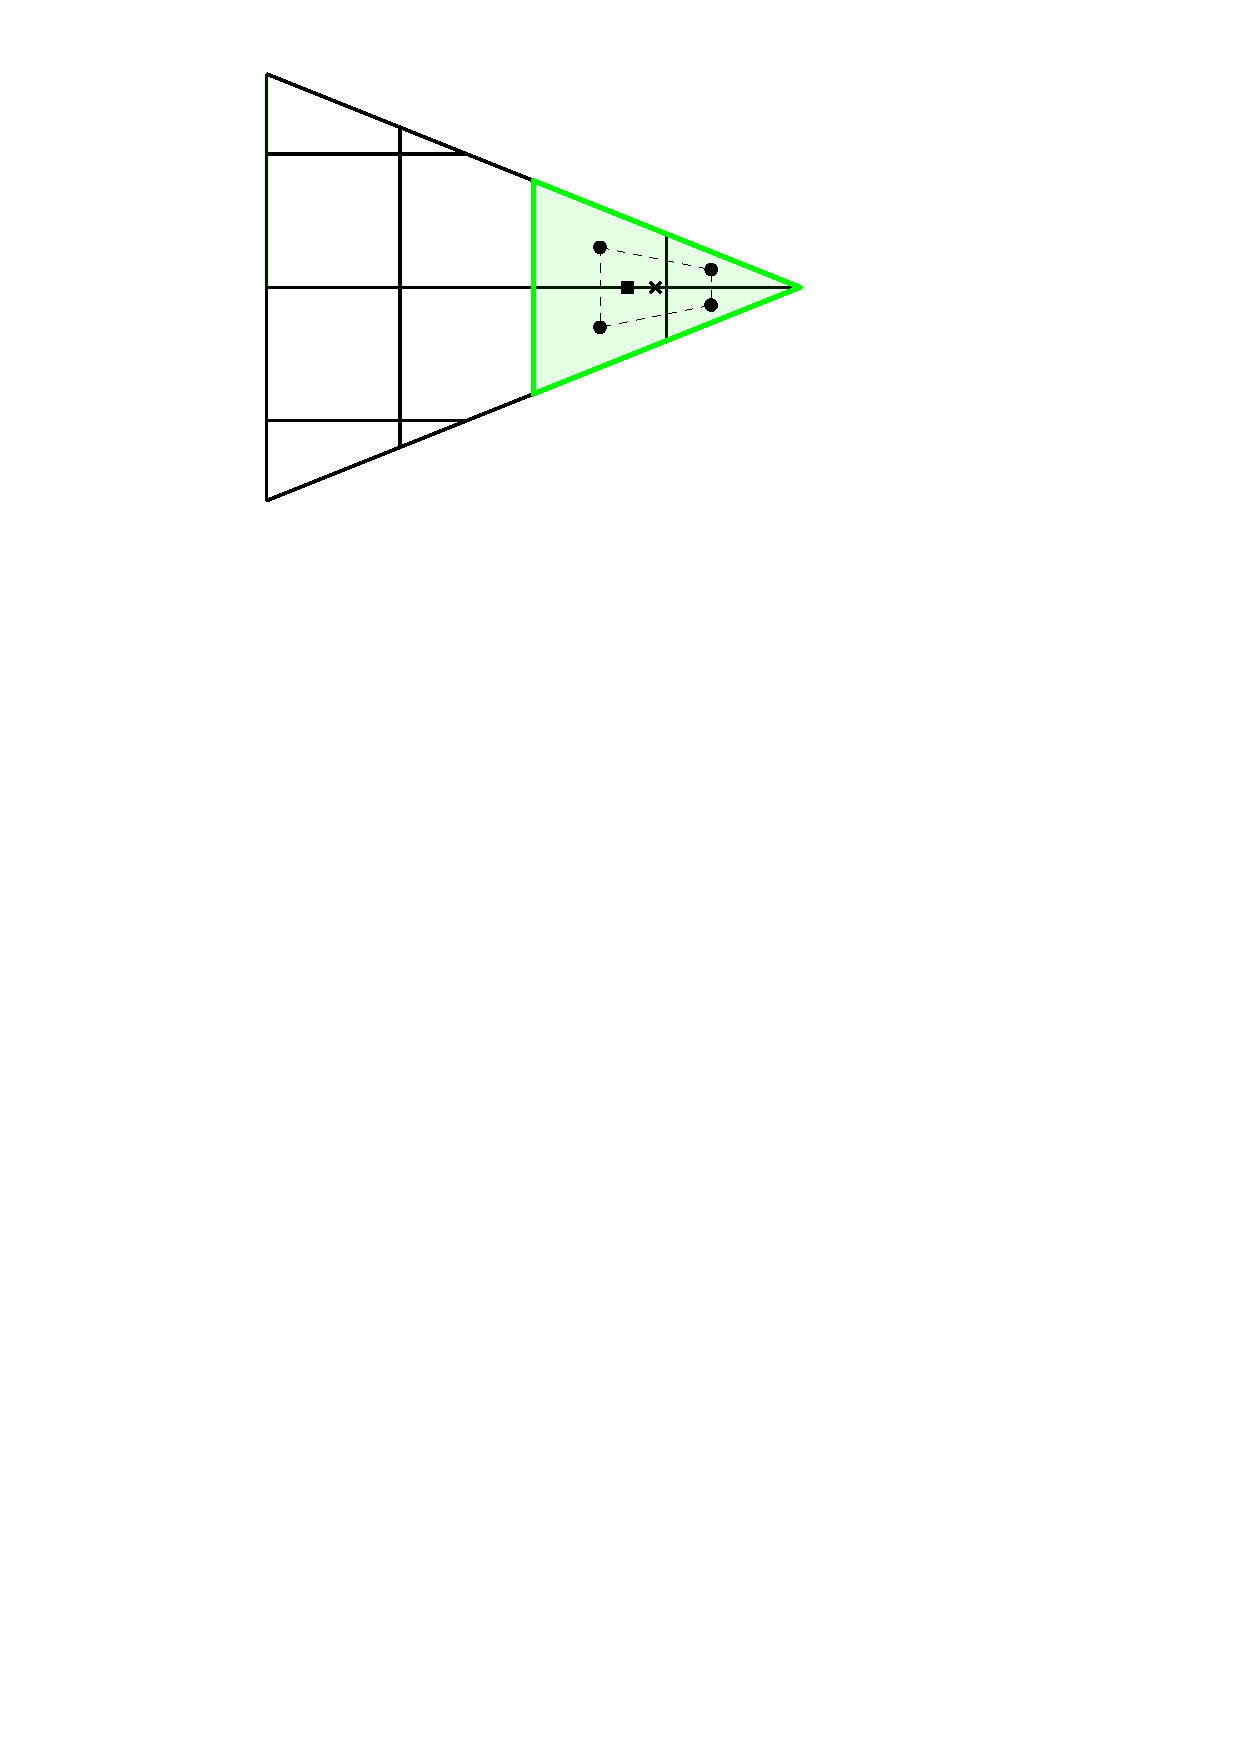
\includegraphics[width=0.45\linewidth]{figs/centroids4.pdf}}
    \caption{\sf The centroids of the Cartesian and cut cells are indicated with a solid circle ($\bullet$).  The centroids and weighted centroids of the merging neighborhoods are indicated with a square ($\blacksquare$) and a cross ($\times$), respectively. Note that the centroids and weighted centroid of the cut cell neighborhoods do not necessarily coincide.}
    \label{fig:centroids}
\end{figure}
The reconstruction neighborhood for $i,j$ is initialized to the $3 \times 3$ tile centered on $i,j$.
With this choice, it could happen that the centroids are too close to each other to compute a gradient in the normal direction (figure \ref{fig:tooclose}). If the weighted centroids are not at least $0.5\,\Delta x$  and $0.5\,\Delta y$ apart in the $x$ or $y$ direction then we increase the stencil size for the gradient computation.  For example, if the weighted centroids are too close in the $x$ direction, but not the $y$ direction, then the $5\times 3$ tile is used as the reconstruction neighborhood.  Similarly, if the weighted centroids are too close in the $y$ direction, but not the $x$ direction, then the $3\times 5$ tile is used as the reconstruction neighborhood.  The neighborhood size is increased until the distance constraint is satisfied in both directions.  In figure \ref{fig:tooclose}, the appropriate reconstruction neighborhood is $3\times 5$ reconstruction tile.
% The same neighborhood that is used for computing the gradient can be used to limit the gradient to prevent overshoots. The centroid is computed using the same weighting by number of neighborhoods as when the volume was computed. (IS THIS TRUE AND IS IT NECESSARY) NEED DISCUSSION OF NOT A REAL CENTROID
% For most full cells with a count of one, the normal gradient computation as done in the finite volume update will suffice.

\begin{figure}
    \centering
    \subfloat[]{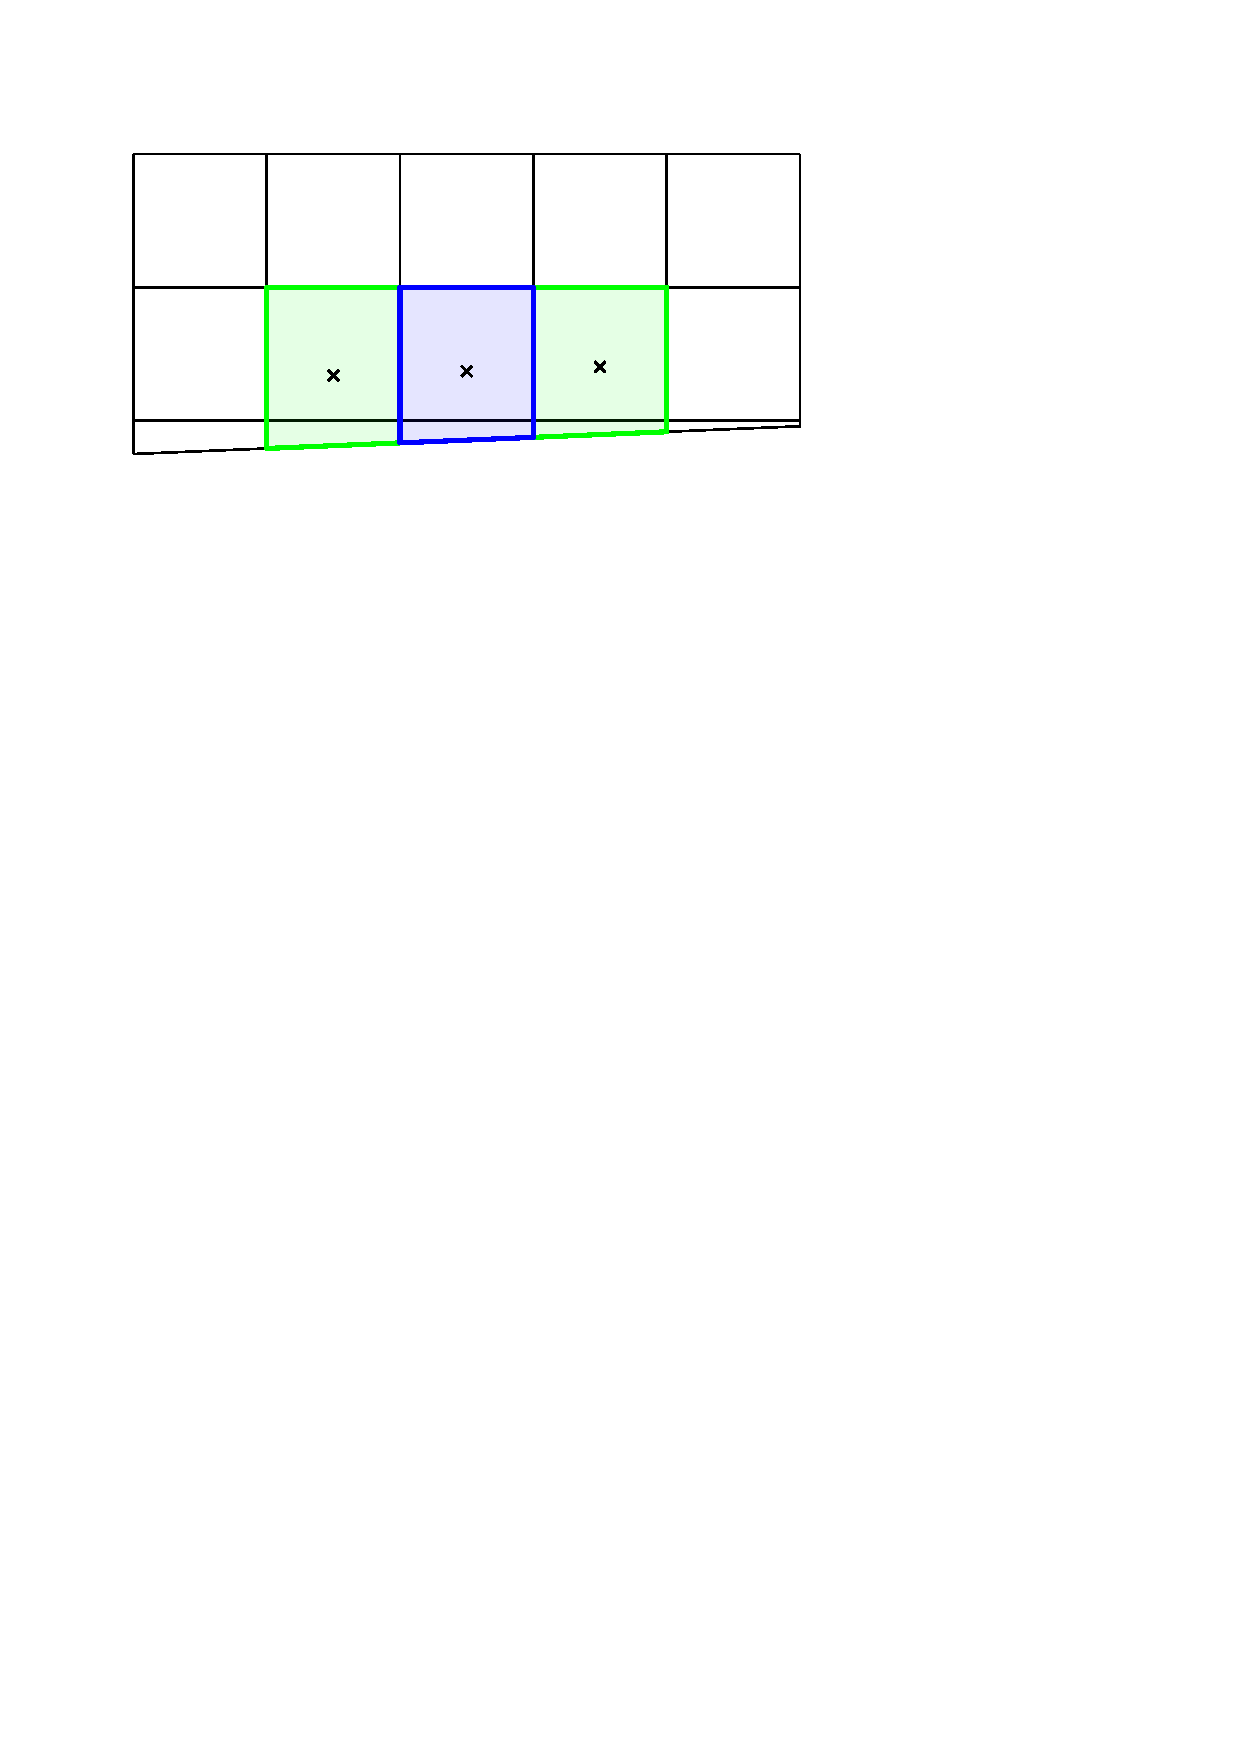
\includegraphics[width=0.45\linewidth]{figs/tooclose2.pdf}} \hfill
    \subfloat[]{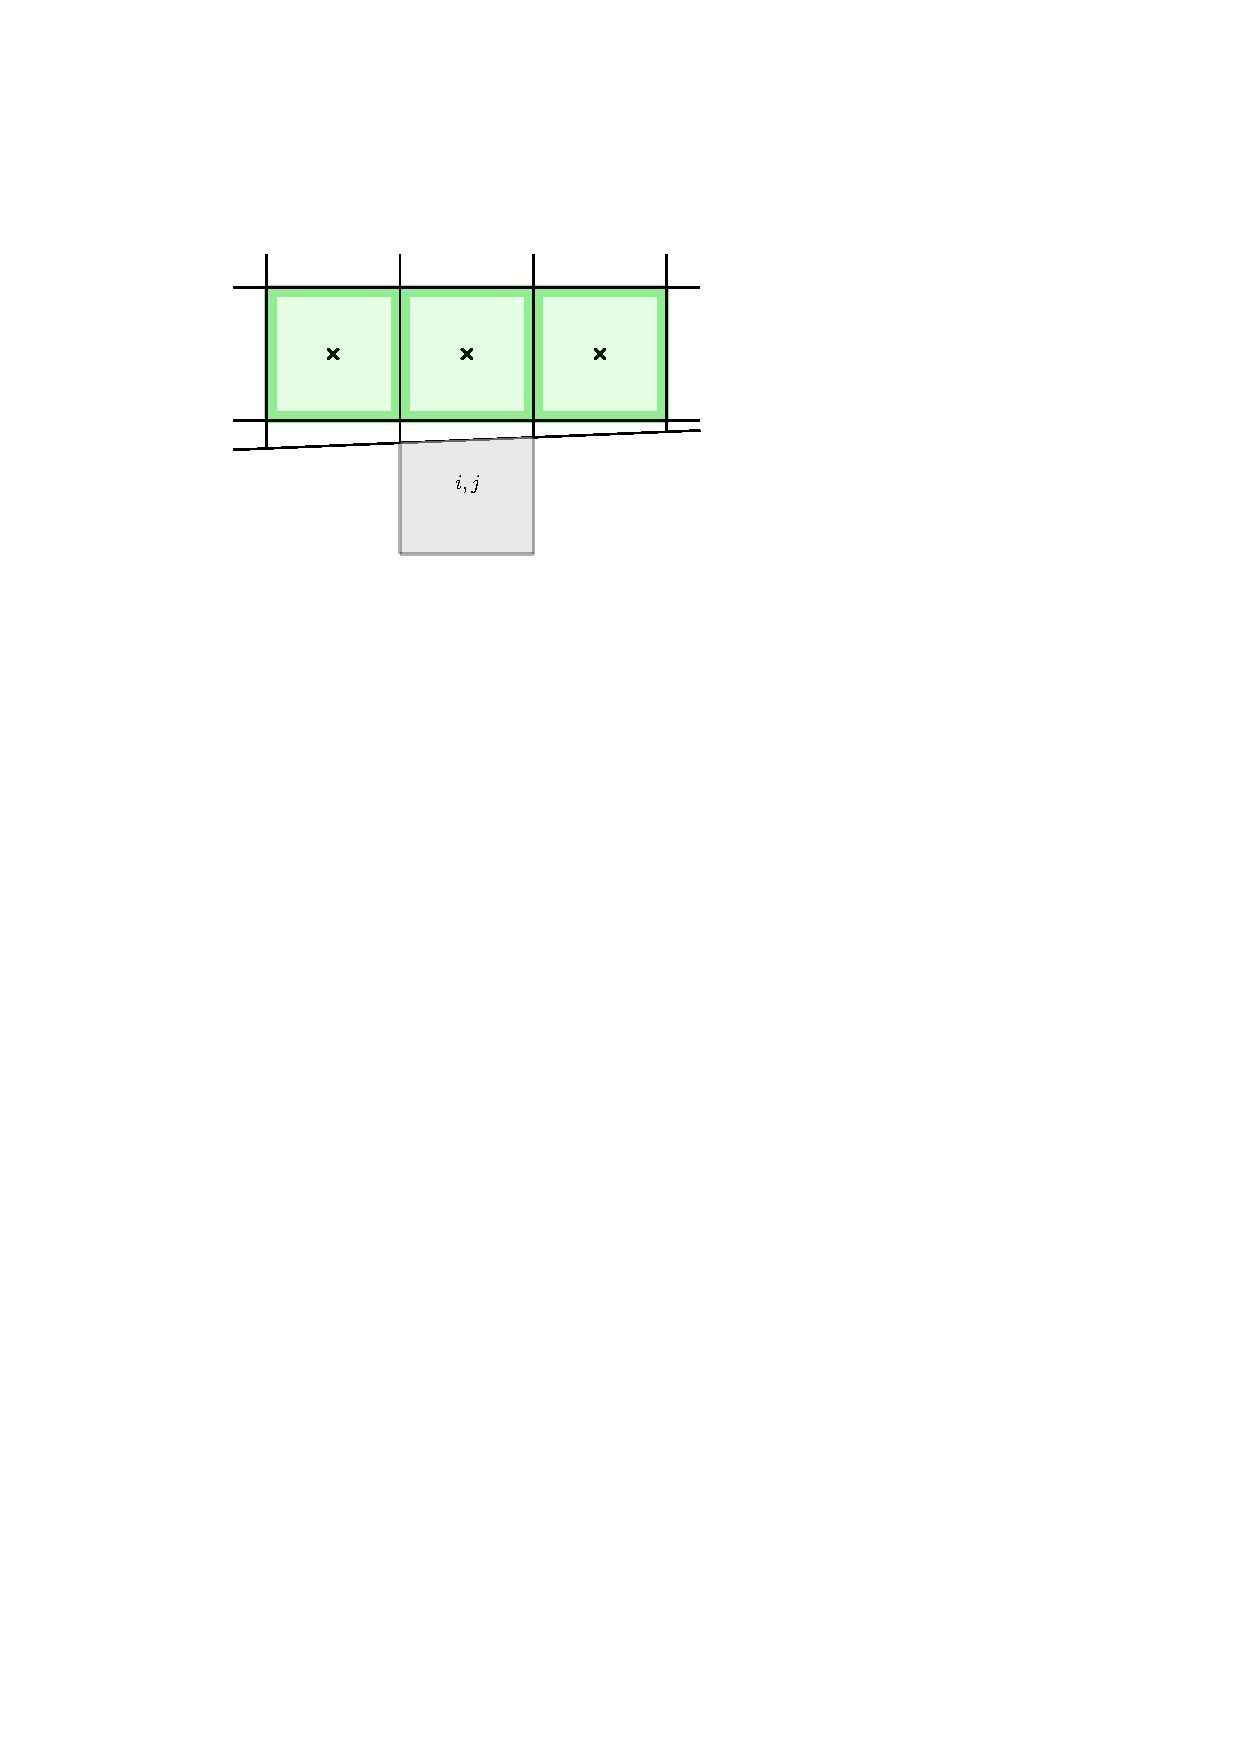
\includegraphics[width=0.45\linewidth]{figs/tooclose1.pdf}} 
    \caption{\sf The blue cell's $3\times3$ reconstruction tile highlighted in green.  The weighted centroids are indicated with a cross ($\times$).}
    \label{fig:tooclose}
\end{figure}

\item
{\bf Replace the provisionally computed cut cell values and their adjacent
full cell neighbors with  the contributions from the merged tiles.} 

\vspace*{.1in}
The final solution at time $t^{n+1}$ on cut cell $i,j$ is obtained by compiling a the indices of all merging neighborhoods that overlap cell $i,j$ in the set $W_{i,j}$.  Then, the solution on merging neighborhood $k,l$ in $W_{i,j}$ is evaluated at $i,j$'s physical centroid, $x_{i,j}$, given by $\hat{q}_{k,l}(x_{i,j})$.  The final solution value on cell $i,j$ is given by the average of these values, i.e.,
\begin{equation} \label{eq:final_update_linear}
U^{n+1}_{i,j} := \frac{1}{N_{i,j}}\sum_{(k,l) \in W_{i,j}}\hat{q}_{k,l}(x_{i,j}).
\end{equation}
To use the example of figure \ref{fig:2nborTile}, the cut cell value
\begin{equation}
   U_{i,j}^{n+1} := \widehat{Q}_{i,j} 
   + (x_m - x_{i,j}) \, \frac{\partial \widehat{Q}_{i,j}}{\partial x} 
   + (y_m - y_{i,j}) \, \frac{\partial \widehat{Q}_{i,j}}{\partial y}
\end{equation}
since cell ${i,j}$ only belongs to one neighborhood. The adjacent full cell
on the other hand belongs to two neighborhoods -- the one it shares with
the cut cell $i,j$ , and its own merging neighborhood.
So its solution at time $t_{n+1}$  becomes
\begin{equation}
\label{eqn:numhood2ex}
\begin{split}
   U_{i,j+1}^{n+1} \,=\, & \frac{1}{2}\widehat{q}_{i,j}(x_{i,j})+ \frac{1}{2} \widehat{q}_{i,j+1}(x_{i,j}), \\
   = &\frac{1}{2} \left
   (\widehat{Q}_{i,j} 
   + (x_m - x_{i,j+1}) \, \frac{\partial \widehat{Q}_{i,j}}{\partial x} 
   + (y_m - y_{i,j+1}) \, \frac{\partial \widehat{Q}_{i,j}}{\partial y} \right ) + \frac{1}{2} \widehat{Q}_{i,j+1} .
\end{split}
\end{equation}
The last term  in eq. \eqref{eqn:numhood2ex} has no gradient terms because the
centroids of the original cell and merged cell are identical.
The fraction $\frac{1}{2}$ is because cell $(i,j+1)$ is part of  two
neighborhoods, so each contributes half of the solution.
\end{enumerate}

Different choices of neighborhoods, the minimum volume for the merging
neighborhood, gradient neighborhoods, and limiting will give
somewhat different computational results. Some of these will be examined
theoretically using model problems in one space dimension in section
\ref{sec:theory}. These choices can affect the stability limit of the
overall method.
We will also show computational results using different neighborhood
choices in section \ref{sec:compResults} in two space dimensions.

The conservation properties of the algorithm will be discussed after the
higher order SRD algorithm is presented in the next
section (PR PUT IT HERE). It will also be prseented more generally.   
OTHER THINGS HERE? DEMONSTRATE LINEARLY EXACT SECOND ORDER CONVERGENCE
HERE INSTEAD OF COMPRESULTS SECTION?

% SOMEHWERE PUT IMPLEMENTATION SUBSECTION OR AT LEAST A PARAGRAPH
% TO NOTE THAT THE CELL DOESNT KNOW WHO GIVES TO
% IT, SO THIS LOOP IS OVER GIVERS  NOT RECEIVERS.
The final update formula \eqref{eq:final_update_linear} can easily be implemented with a nested for loop in algorithm \ref{alg:finalupdate}.  
The outer loop iterates over the merging neighborhoods $i,j$ and the inner loop iterates over each cell $k,l$ in merging neighborhood $i,j$.  Each merging neighborhood $i,j$ gives a contribution $ \hat{q}_{i,j}(x_{k,l})/N_{k,l} $ to the cells $k,l$ that belong to it.
\begin{algorithm}[H]
\SetAlgoLined
$U^{n+1}(:,:) := 0$\\
 \ForAll{$i,j$}{
     \ForAll{$(k,l) \in M_{i,j}$}{
        $U^{n+1}(k,l) := U^{n+1}(k,l) + \hat{q}_{i,j}(x_{k,l})/N_{k,l} $
     }
 }
 \caption{\sf Final solution update} \label{alg:finalupdate}
\end{algorithm}

\begin{figure}
	\subfloat[]{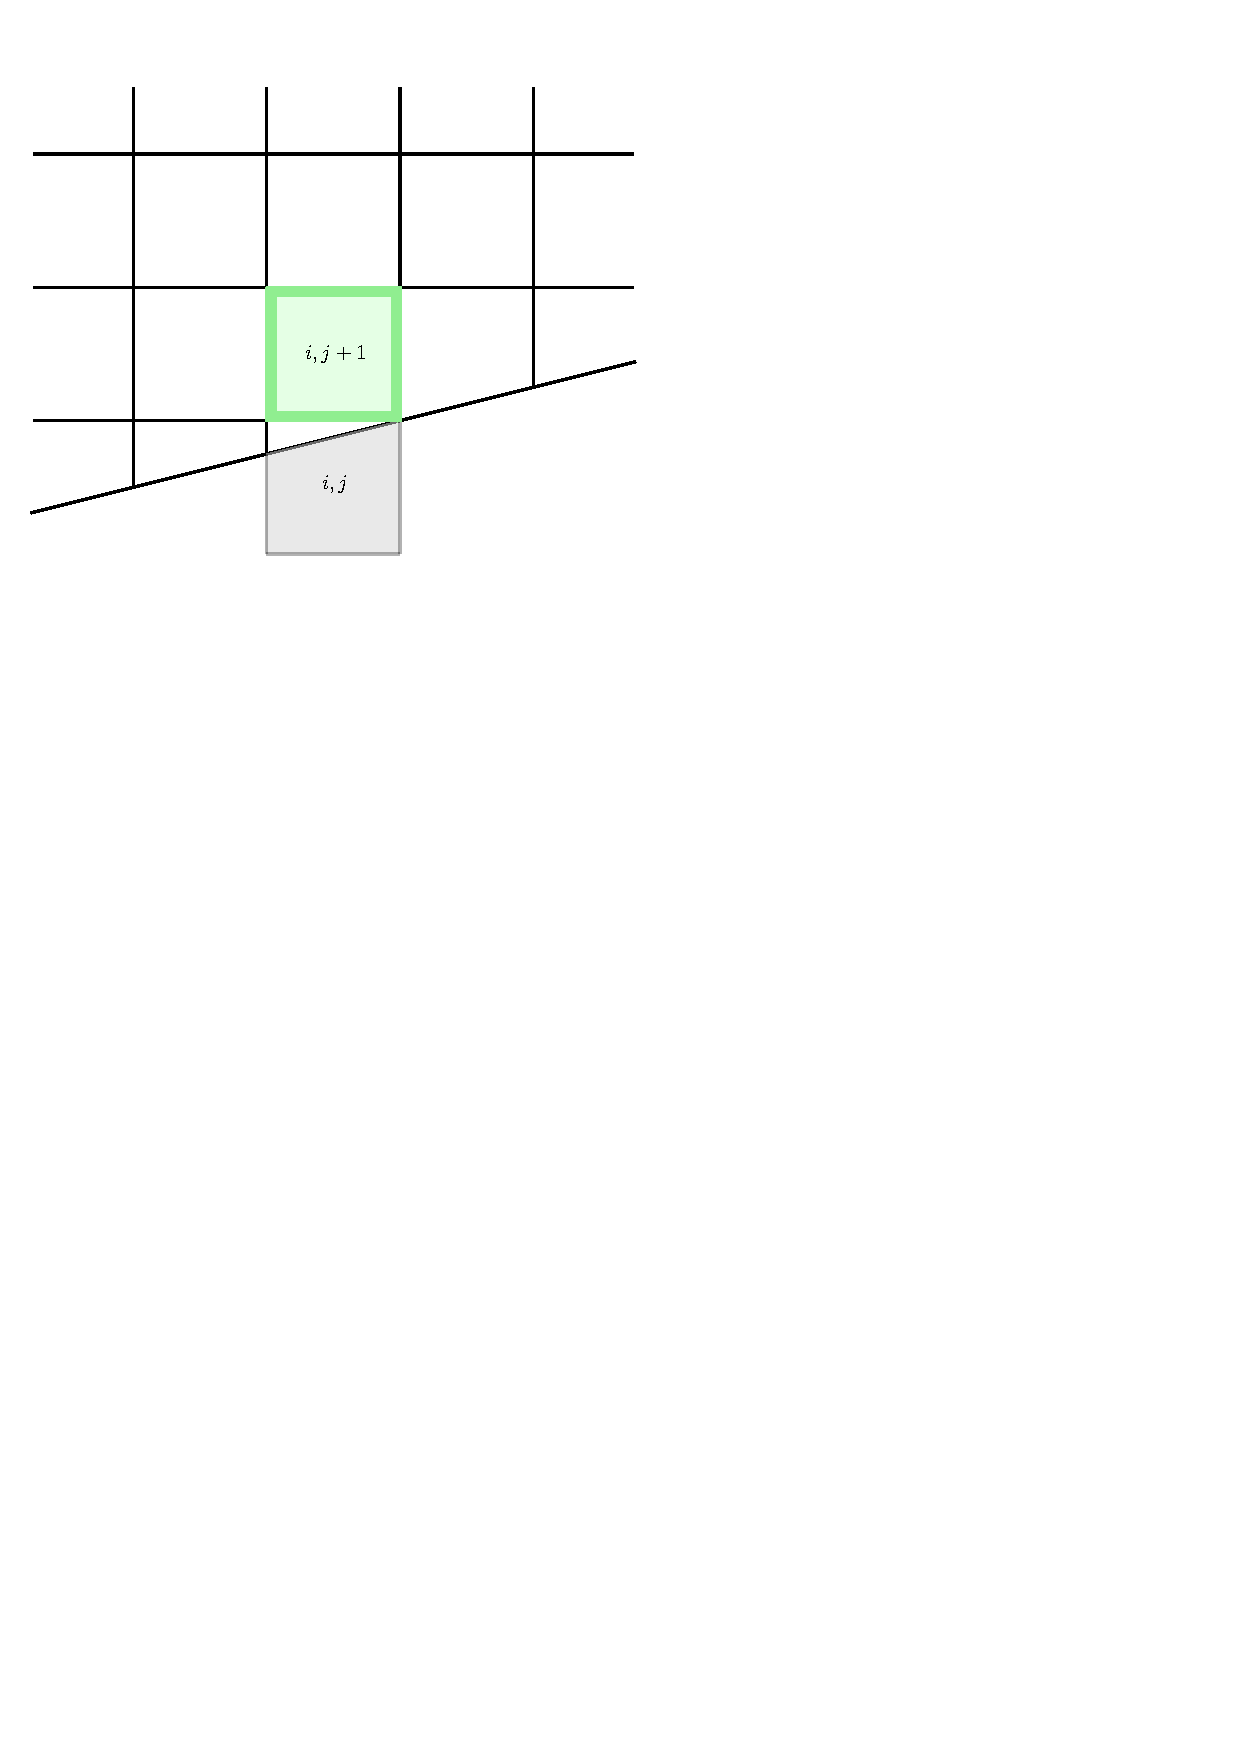
\includegraphics[width=0.45\textwidth]{figs/modelexample2D_1.pdf} \label{fig:2nborTile1}}
	\hfill
	\subfloat[]{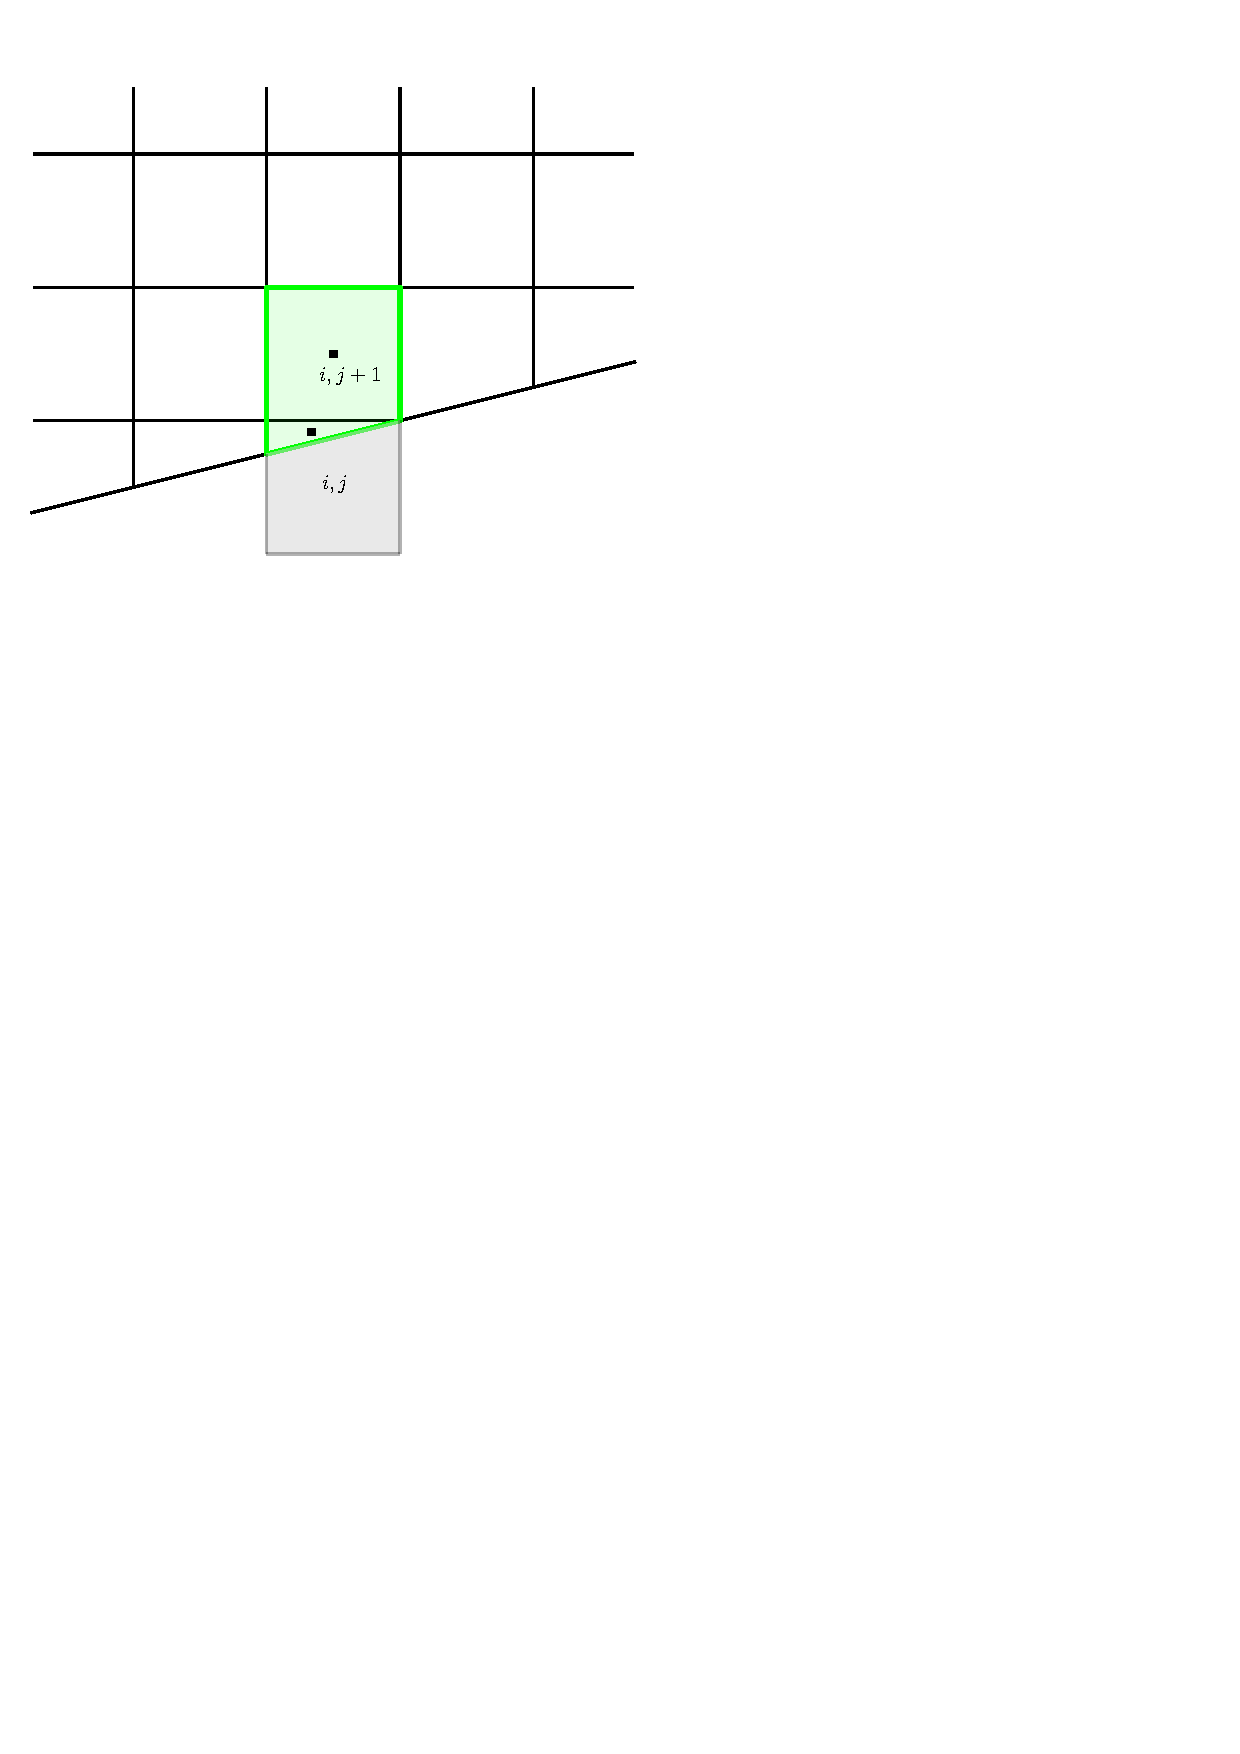
\includegraphics[width=.45\textwidth]{figs/modelexample2D_2.pdf} \label{fig:2nborTile2}}
	\caption{\sf Two-dimensional example of overlapping neighborhoods.  The unweighted centroids of cells $i,j$ and $i,j+1$ are indicated with solid squares ($\blacksquare$).} \label{fig:2nborTile}
\end{figure}


\subsection{Limiting on merging neighborhoods}
In this section we design a linearity preserving limiter for slopes on merging neighborhoods.  Designing a limiter that does not destroy the linearly preserving property is not so straightforward.  
%We demonstrate this
%In particular, we apply the LP limiter [] on slopes

\section{Computational Results}\label{sec:compResults}
In this section we show several computational experiments using state
redistribution to solve the Euler
equations. We will also use these
examples to examine 
properties of different gradient choices and base schemes. 
%We solve the conservation law \eqref{eq:conslaw2D} with different fluxes $\mathbf{F}$, to include both smooth and discontinuous
%solutions.

%\subsection{Linear fluxes}
%\subsubsection{Linear convergence study}
%We solve \eqref{eq:conslaw2D} with the flux $\mathbf{F}(u) = [-2\pi y u, 2\pi x u]$ and initial condition
%$$
%u_0(x,y) = w(\theta - \pi/2)
%$$
%where
%$$
%w(\theta) = \frac{1}{2}\left( \text{erf}\left( \frac{\pi/6 - \theta}{\sqrt{4/100}} \right) + \text{erf}\left( \frac{\pi/6 + \theta}{\sqrt{4/100}} \right)\right)
%$$
%until the final time $T = 1$ on the domain enclosed by two concentric disks of 
%radii $R_1 = 0.751$ and $R_2 = 1.251$.  
%Figure \ref{fig:rotatinghillgrid} shows the computational domain 
%embedded in a $50 \times 50$ grid.  The exact solution is the initial condition 
%rotated about the point $(1.5,1.5)$, where $T=1$ corresponds to one solid 
%body rotation. This example IS FROM \cite{}, for comparison.  (AND ADD
%COMPARISON - ARE THEY OR WE MORE ACCURATE< BUT WE ARE EASIER).   
%The errors 
%measured in the $L_1$ and $L_\infty$ norms are provided in 
%Tables \ref{tab:ex1_L1} and \ref{tab:ex1_Linf}.  Figure
%\ref{fig:rotatinghillexactiso} shows isolines of solution at the initial 
%and final time.  The exact solution is applied as the boundary condition.
%CHEATING?
%This problem is solved using the finite volume TVD-RK2 scheme. 
%
%\begin{figure}
%\subfloat[$50\times50$ grid and annulus domain.]{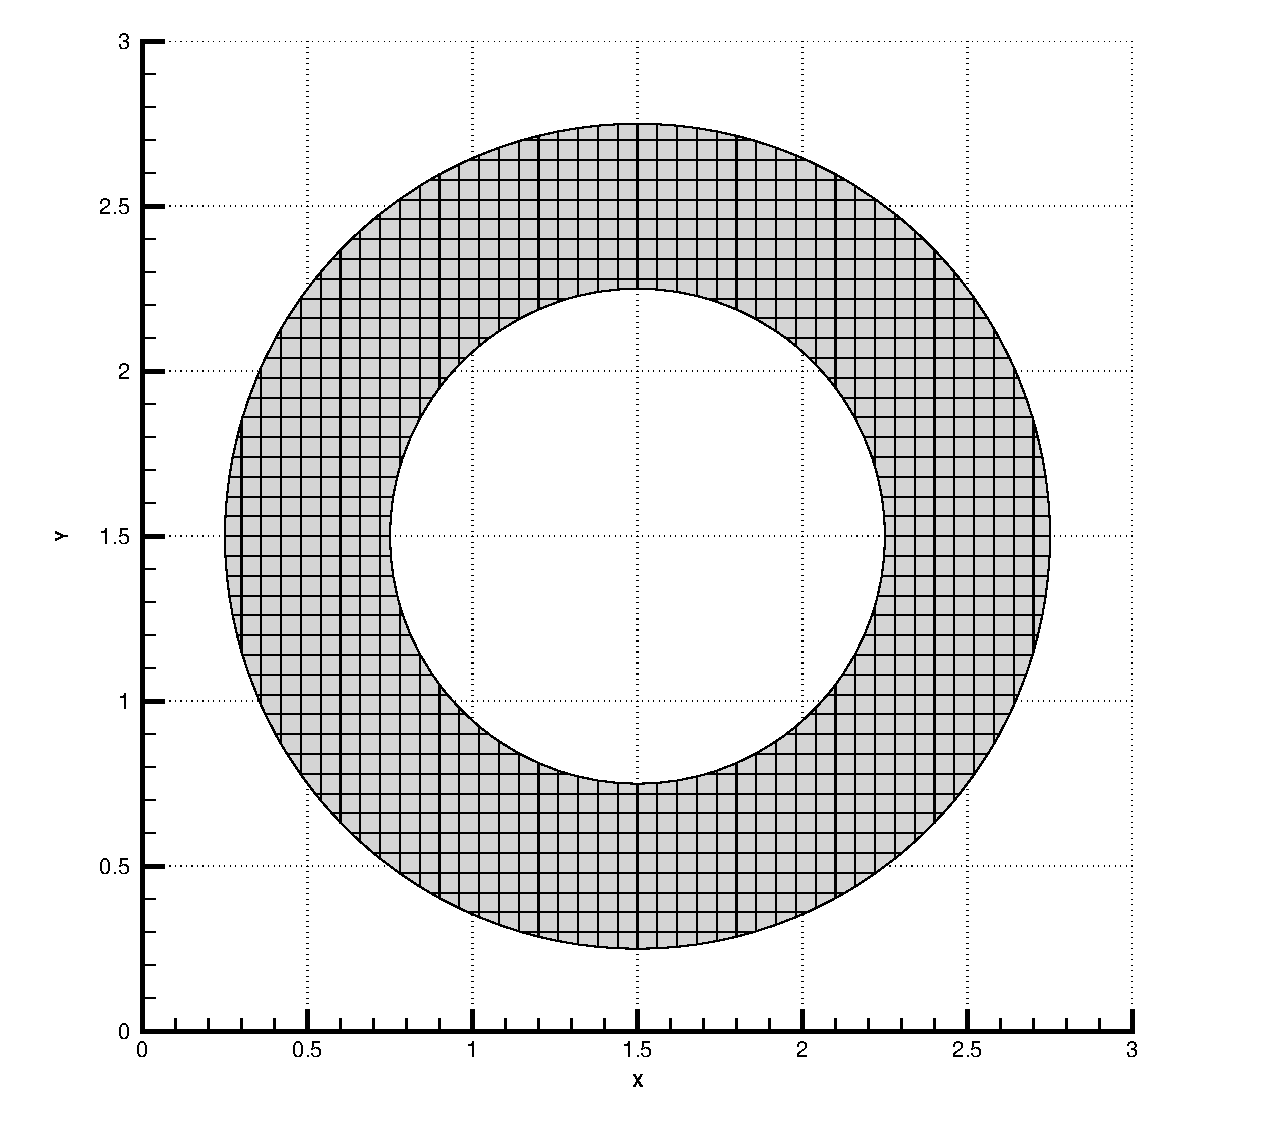
\includegraphics[width = 0.5\linewidth]{figs/rotatinghill_grid.eps} \label{fig:rotatinghillgrid}} 
%\quad
%\subfloat[Isolines of exact solution at the initial and final time. SHOW
%COMPUTED SOLUTION TOO]{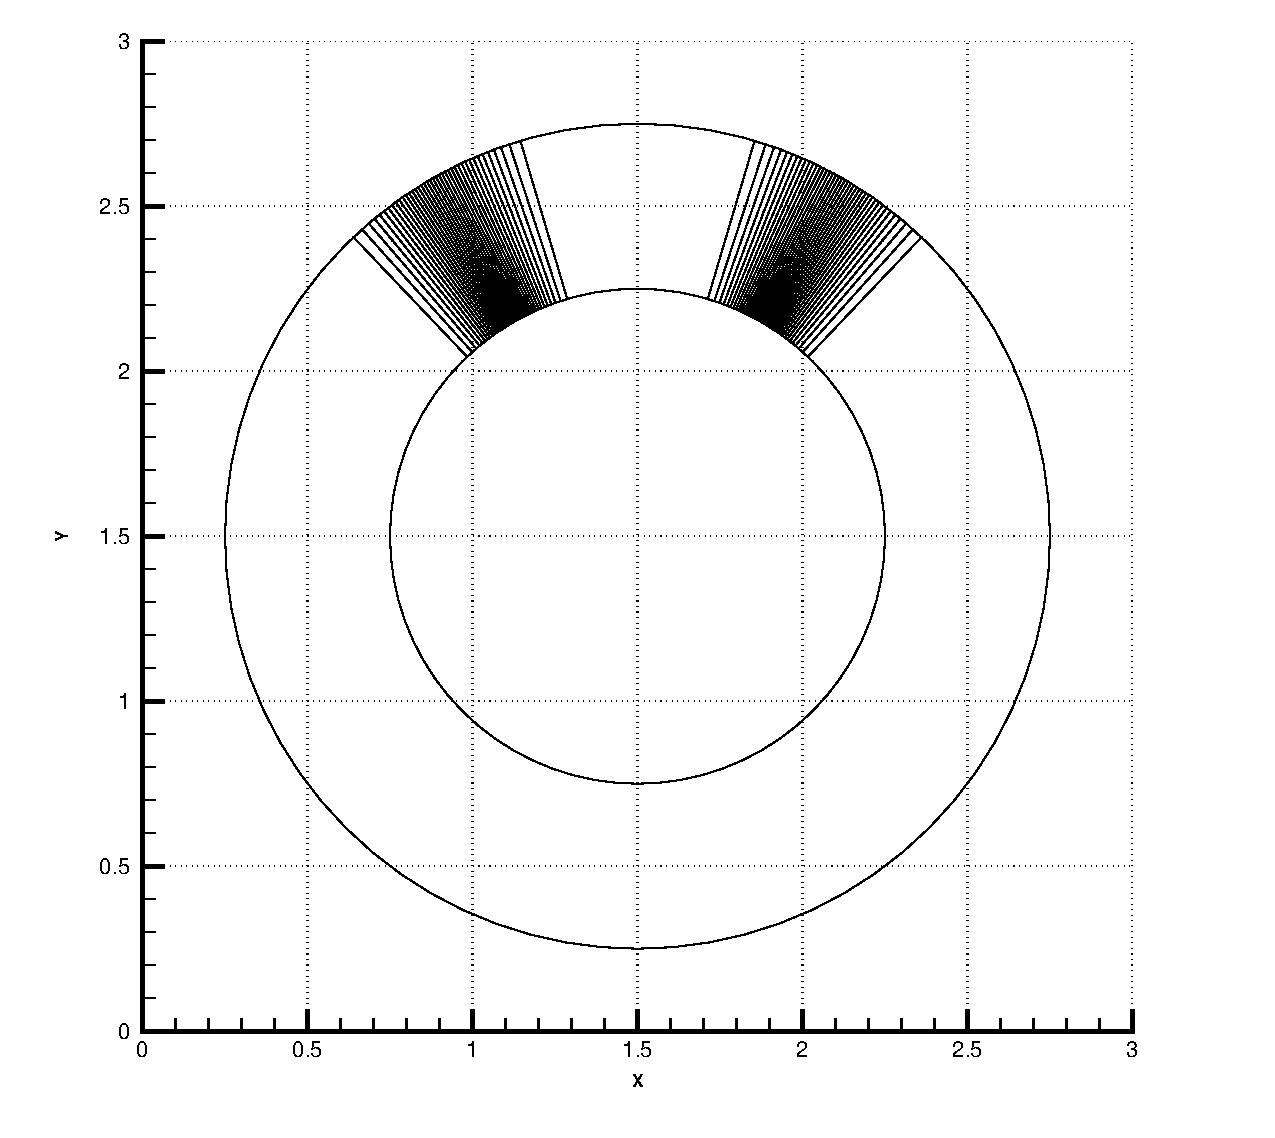
\includegraphics[width = 0.5\linewidth]{figs/rotatinghill_solution.eps}\label{fig:rotatinghillexactiso}}
%\end{figure}
%    % \caption{}\label{tab:ex1_L1}
%
%{\large
%\begin{table}
%\centering
%\subfloat[$L_1$ errors. \label{tab:ex1_L1}]{
%    \begin{tabular}{|c|c|c|c|c|}
%        \hline
%         $N_x \times N_y$ & $p = 0$ & $p=1$& $p=2$ & $p=3$ \\
%         \hline
%         50 & 2.3937e-1(-) &  5.6588e-2  (-)& 4.1690e-2  (-)&   2.0694e-2 (-)\\
%         \hline
%         100 &  1.5521e-1 (0.62) &  2.0125e-2  (1.49)& 7.8165e-3 (2.41)& 1.6813e-3 (3.62)\\
%         \hline
%         200 &  9.4138e-2 (0.72) & 5.5222e-3 (1.86)&  9.98411e-4 (2.96)& 8.8527e-5 (4.24)\\
%        %  \hline
%        %  400 &  () &  ()&  ()&  ()\\
%         \hline
%    \end{tabular}
%    }
%\quad
%\subfloat[$L_\infty$ errors. \label{tab:ex1_Linf}]{
%    \begin{tabular}{|c|c|c|c|c|}
%        \hline
%         $N_x \times N_y$ & $p = 0$ & $p=1$& $p=2$ & $p=3$ \\
%         \hline
%         50 & 3.0385e-1 (-) &  1.6856e-1 (-)& 1.1809e-1 (-)&  7.0682e-2 (-)\\
%         \hline
%         100 & 2.3332e-1 (0.38) & 8.5487e-2 (1.04)& 5.1249e-2 (1.20)& 1.6657e-2 (2.08)\\
%         \hline
%         200 &  1.7698e-1 (0.39) & 3.4940e-2 (1.29)& 1.4500e-2 (1.82)&  1.9507e-3 (3.09)\\
%        %  \hline
%        %  400 &   () &  ()&  ()&  ()\\
%         \hline
%    \end{tabular}
%    }
%
%\caption{Errors for the linear convergence study. ADD METHOD DETAILS TO
%DESCRIPTION - USED WHICH GRADIENT RECON. ADD 400 POINTS}
%\end{table}
%}
%
%\subsubsection{Overlapping neighborhoods}
%The purpose of this example is to demonstrate that our algorithm can handle a substantial number of overlapping neighborhoods.  
%Using the streamfunction
%$$
%\phi = R - 0.25\sin(10\theta),
%$$
%with $R = \sqrt{(x-1.5)^2+(y-1.5)^2}$ and $\theta = \arctan((y-1.5)/(x-1.5))$, we define a linear flux based on the resulting divergence free velocity field, i.e.,  $\mathbf{F}(u) = [\phi_y u, -\phi_xu]$.  The characteristics of \eqref{eq:conslaw} lie on the isolines of the streamfunction.
%
%A steady state solution to \eqref{eq:conslaw} with the above flux is given by the streamline function.  Therefore, we start with the initial condition given by the streamline function $\phi$, and compute the solution until the final time $T = 10$ on a $100 \times 100$ grid.  Additionally, we set the flux normal the domain boundary $\mathbf{F}\cdot \mathbf{n} = 0$.  This is to ensure that information does not leave the domain and should solution growth occur, this will more easily be noticed.
%This problem is solved using the finite volume TVD-RK2 scheme. 
%
%
%\begin{table}[h]
%    \centering
%    \subfloat[$L_1$ errors.]{
%    \begin{tabular}{|c|c|c|c|}
%    \hline
%        $p = 0$ & $p =1$ & $p = 2$ & $p =3$  \\
%        \hline
%        3.8585e-1 & 3.6118e-2 & 8.29907e-3 & 4.3116e-3\\
%        \hline
%    \end{tabular} \label{tab:errorsteadystatel1}
%    }
%    \quad
%\subfloat[$L_\infty$ errors.]{
%    \begin{tabular}{|c|c|c|c|}
%    \hline
%        $p = 0$ & $p =1$ & $p = 2$ & $p =3$  \\
%        \hline
%        2.9470e-1 & 9.5323e-2 & 2.4851e-2 &  5.4720e-3 \\
%        \hline
%    \end{tabular}
%    \label{tab:errorsteadystatelinfty}
%    }
%    
%\caption{Errors for overlapping neighborhoods study.} \label{tab:overlappingerrors}
%\end{table}
%
%\begin{figure}[h]
%%\subfloat[Isolines of exact solution at the initial and final time.]{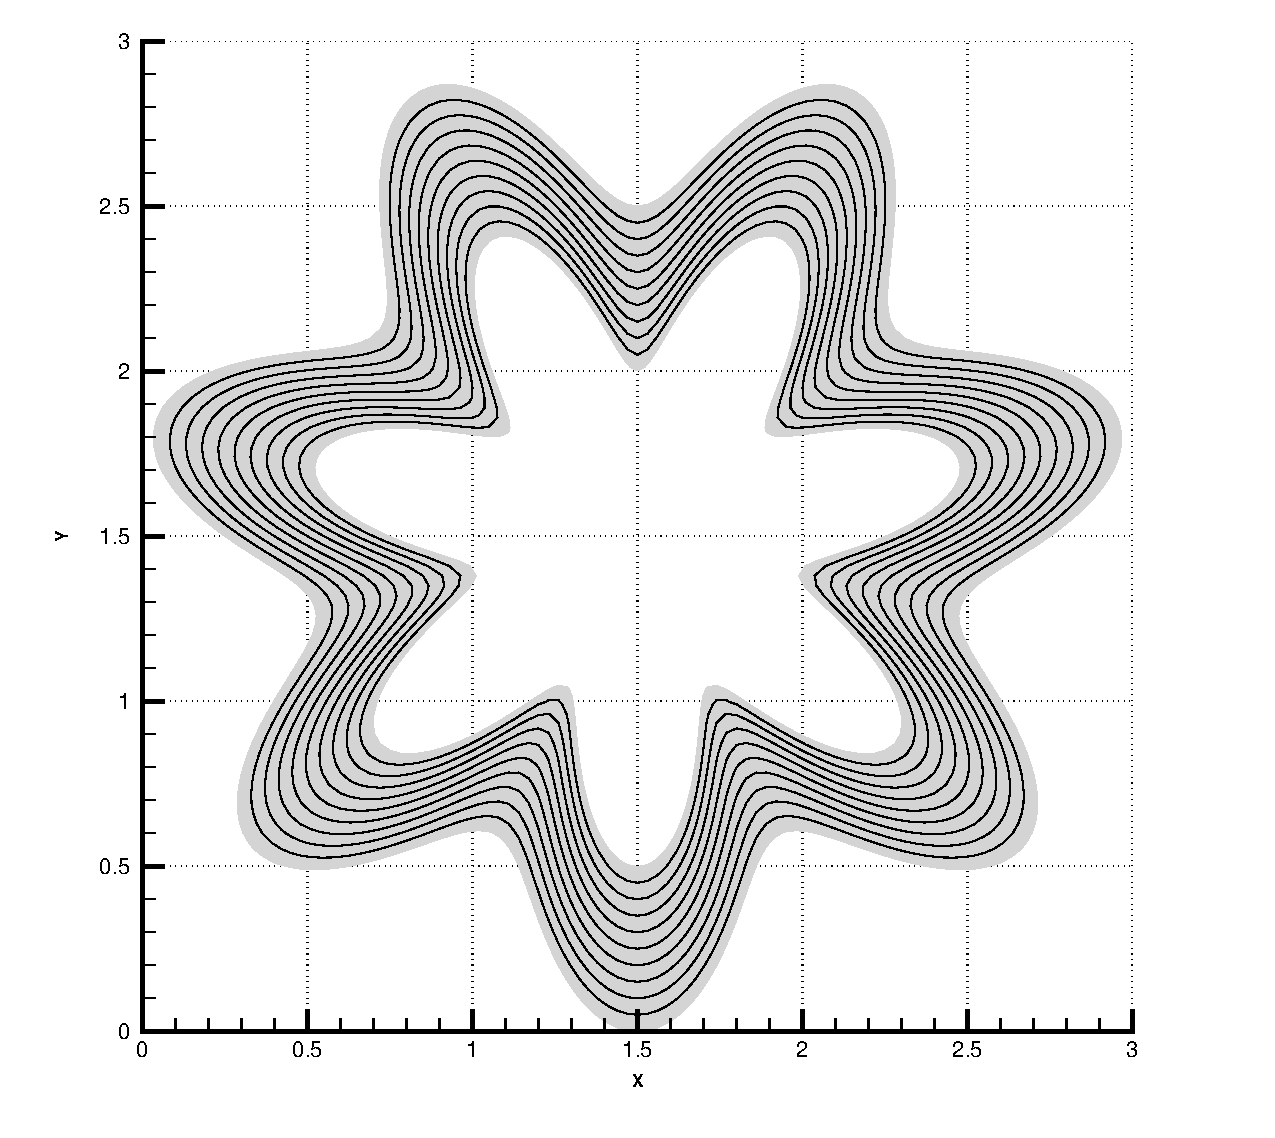
\includegraphics[width = 0.5\linewidth]{figs/waveyiso.eps} \label{fig:waveyisolines}} 
%%\subfloat[Isolines of exact solution at the initial and final time.]{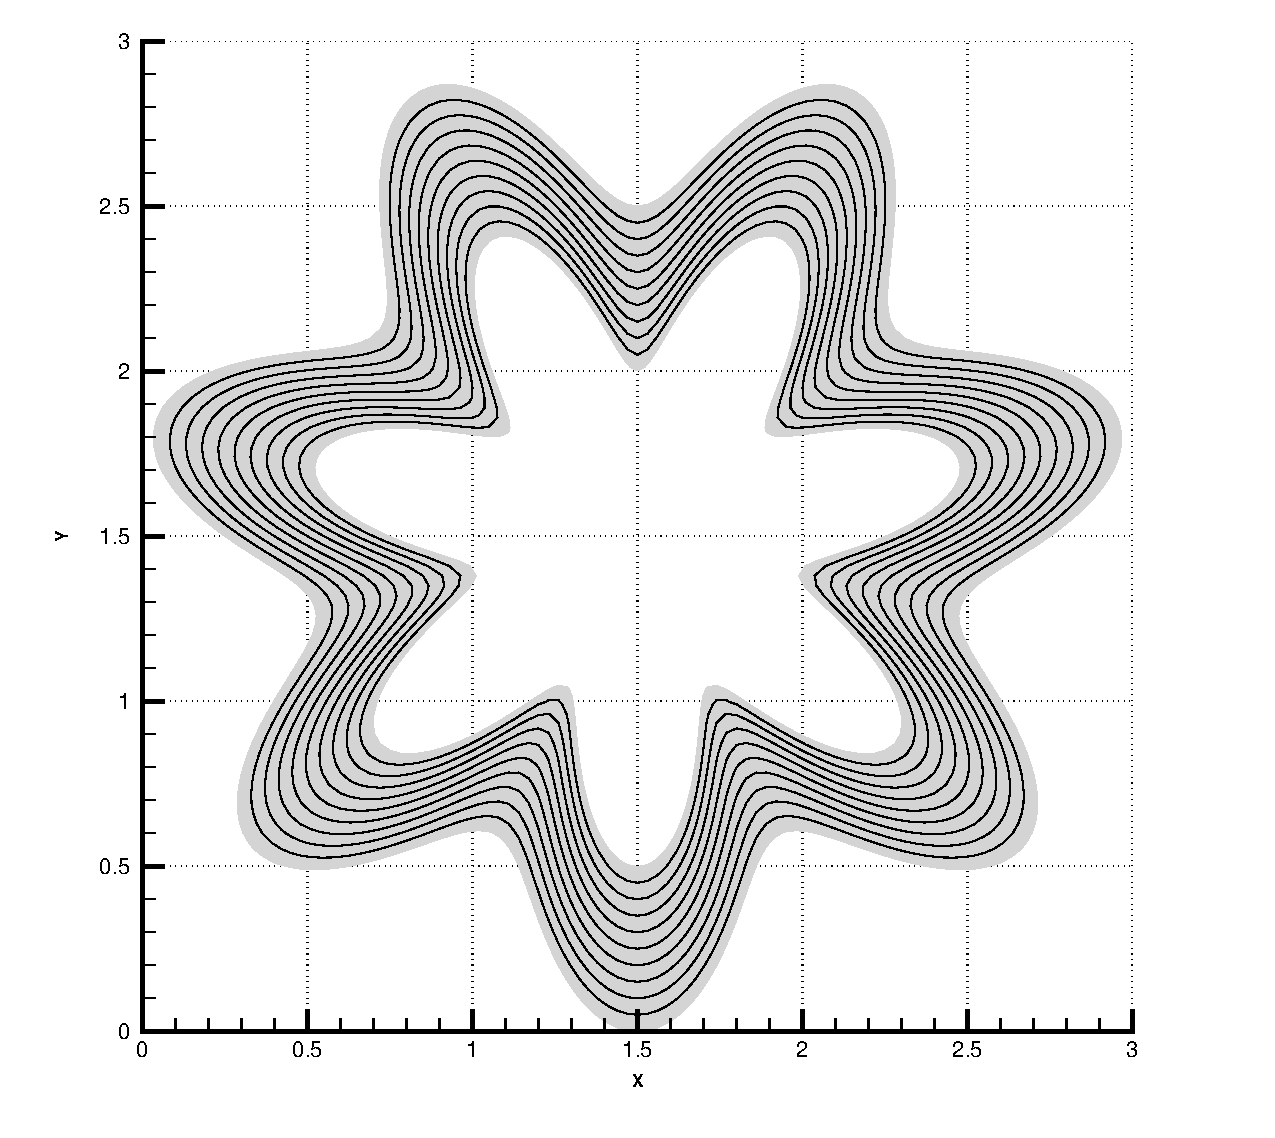
\includegraphics[width = 0.5\linewidth]{figs/waveyiso.eps} \label{fig:waveyisolines}} 
%%\quad
%\subfloat[Number of overlapping merging neighborhoods: one (blue), two (green), three (red).]{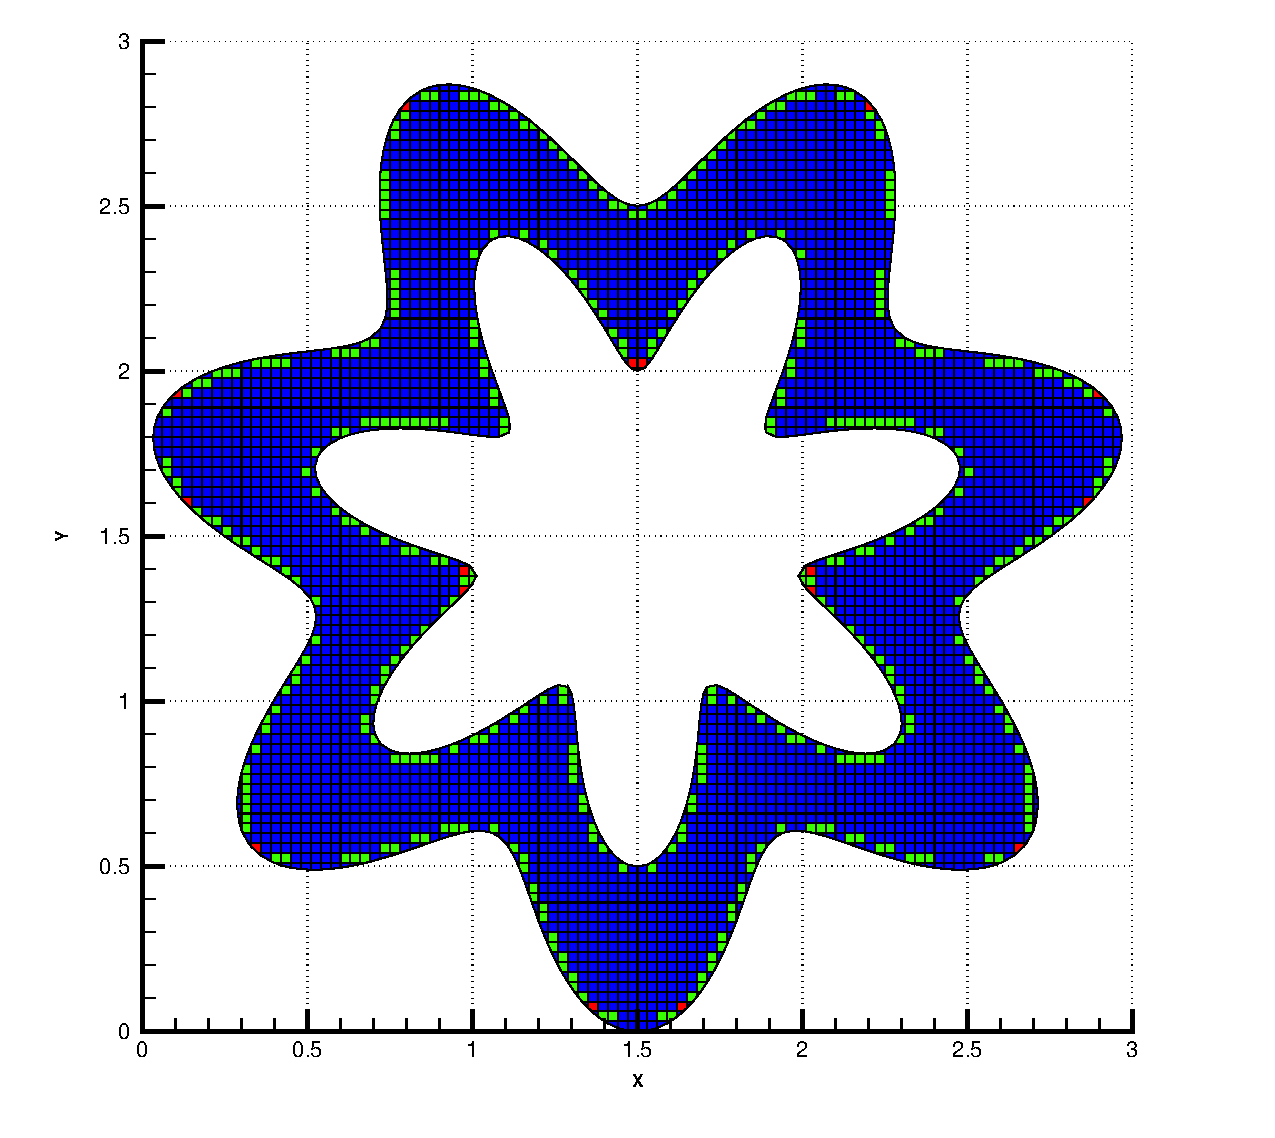
\includegraphics[width = 0.5\linewidth]{figs/waveynumhoods.eps}\label{fig:waveynumhoods}}
%% 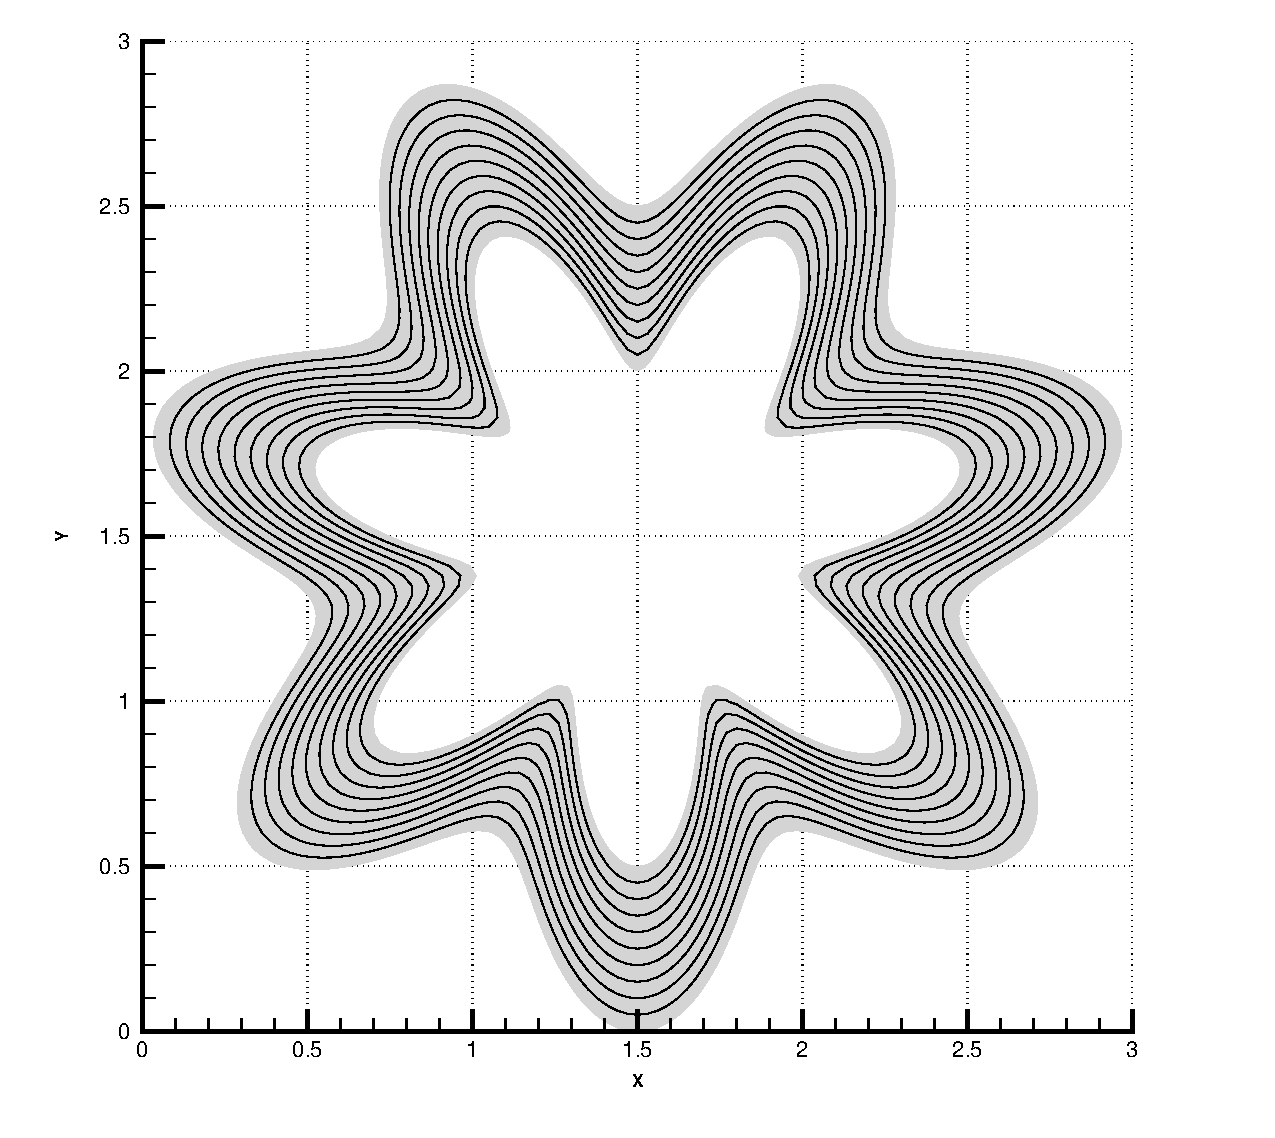
\includegraphics[width = 0.5\linewidth]{figs/waveyiso.eps} 
%\subfloat[Isolines of exact solution at the initial and final time.]{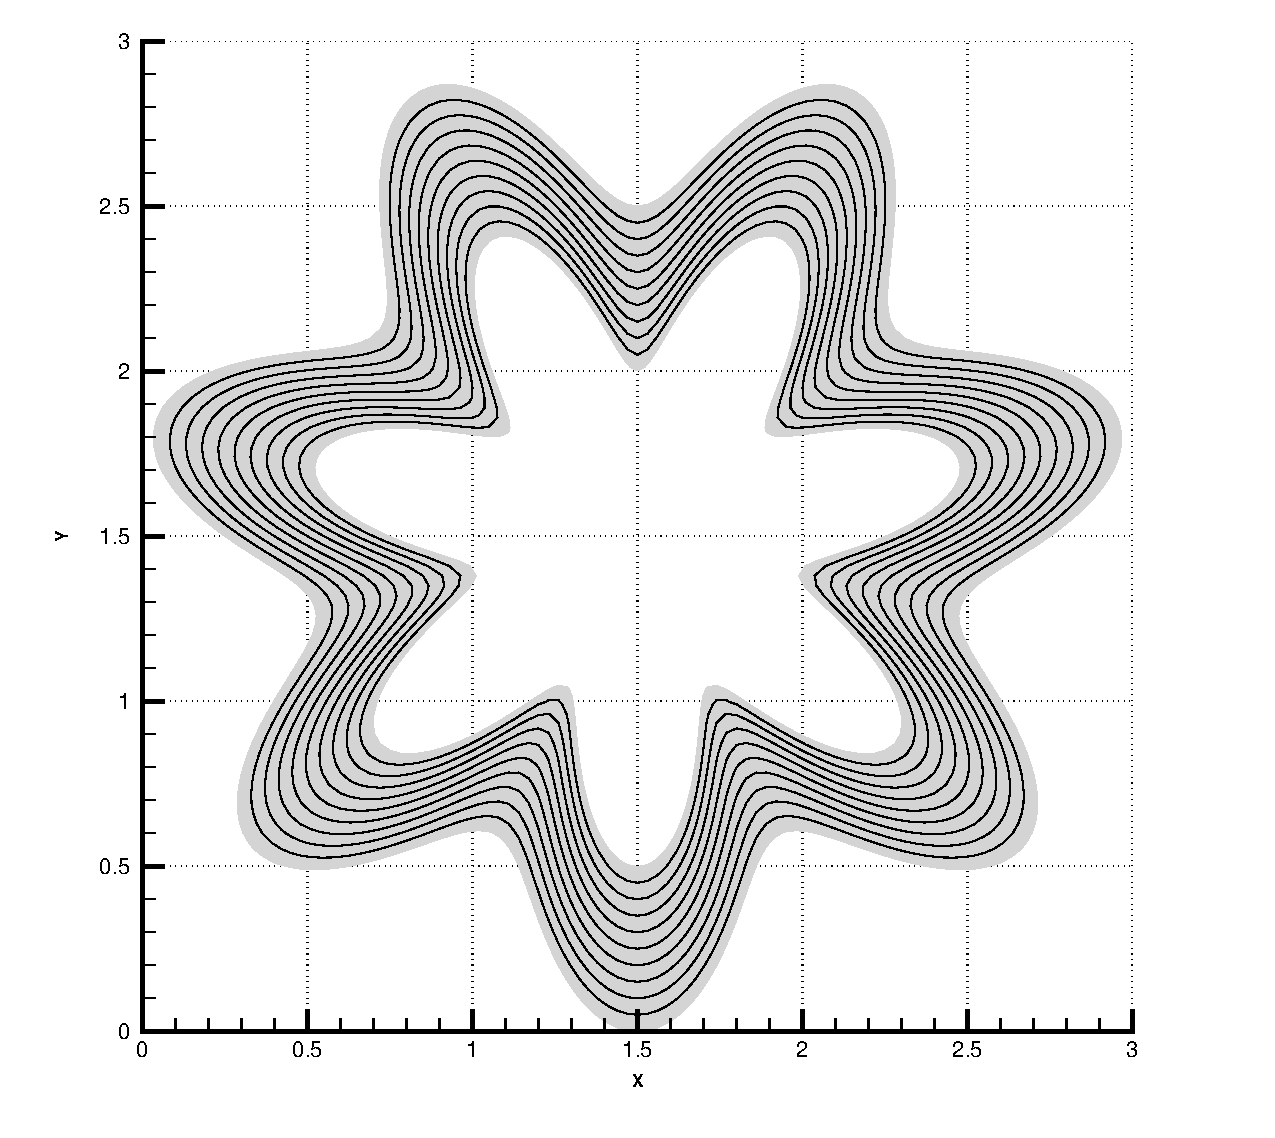
\includegraphics[width = 0.5\linewidth]{figs/waveyiso.eps} \label{fig:waveyisolines}} 
%\caption{Isolines of exact solution at the initial and final time for the
%wavy domain with overlapping neighborhoods. CANT SEE COLORS. WHAT DOES
%THIS EX ADD FROM PREVIOUS ONE} 
%% \label{fig:overlappingneighborhoods}
%% \label{fig:waveyisolines}} 
%\end{figure}
%
%In Figure \ref{fig:waveyisolines}, we show the isolines of the exact solution at the initial and final times.  Additionally, Figure \ref{fig:waveynumhoods} shows the number of overlapping neighborhoods on each cell.  In this example, we have at most three overlapping neighborhoods.  They are concentrated where the boundary has high curvature.   We do not observe growth in the numerical solution as indicated by $L_1$, $L_\infty$ errors of the solution at the final time listed in Table \ref{tab:overlappingerrors}.  Although this experiment does not prove stability of our numerical scheme, not observing unbounded growth in the numerical solution is a necessary condition.


\subsection{Supersonic vortex study}\label{sec:ssv}
We compute the solution to a supersonic flow 
around a quarter circle.  This problem has often been used in accuracy 
studies \cite{aftosmis:acc} since it has an exact solution to the Euler
equations that is smooth, given by 
\begin{equation}
\rho = \rho_i \left \{ 1 + \frac{\gamma-1}{2} \, M_i^2 \left [ 1 - (\frac{r_i}{r})^2
\right ] \right \} ^
{\frac{1}{\gamma-1}}
\end{equation}
and $ u = a_i \, M_i \, (\frac{r_i}{r})\,  \sin (\theta)$, 
$ v = a_i\,  M_i\,  (\frac{r_i}{r})\,  \cos(\theta)$, and
$ p = \rho^\gamma / \gamma$.
Here, the inner radius is $r_i = 1.0$,  the outer radius
is $r = 1.384$, $\rho_i=1$, and the Mach number on the inner circle
$M_i = 2.25$ in our experiments. 
In this
normalization we use $a_i = 1$, $p_i = 1/\gamma$. 
The second order MOL scheme is used, and we march
to steady state, until the maximum density update is below $10^{-10}$.  
The solution is smooth, so no limiters are needed.
The exact solution is used to set the ghost cells at the inflow and
outflow boundaries. The domain size is 1.43 by 1.4301 (slightly different
to prevent mesh  degeneracies).  

In Table \ref{tab:ssv} we compare the accuracy of three different formulations
for the cut cell gradients. 
For first order accurate gradients, we use a linear least squares reconstruction for
both the irregular cell gradient (cut cells and their one-away neighbors) 
described in Section \ref{sec:limit}, and the SRD gradients, which 
update the cut cell solution after stabilization. Second order accurate 
gradients fit a quadratic for both
the cut cells and tiles as described in Section \ref{sec:limit}, 
but only the first derivative terms are used. 
As an intermediate experiment, we  fit a quadratic using least squares but treating the
cell averages as pointwise values at the cell centers. Here again
the second derivative terms are ignored.  Note that this is not
second order accurate, since the centroid value differs by $O(h^2)$
from the pointwise value at the centroid. Nevertheless, this is frequently
done since it is easier to implement, in particular for the SRD neighborhoods
with irregular shapes. 



{
\small
\begin{table}[h]
\centering
	\hspace*{-.3in}
	\subfloat[$L_1$ volume errors. \label{tab:ex1_L1vol}]{
		\begin{tabular}{|l|c|l|l|l|}
			\hline
			$h$ & $N_x, N_y$ & 1st order grad. & ptwise grad. & 2nd order grad.   \\
			\hline
			.5297 & 27 & 6.75e-3 & 2.76e-3 & 2.45e-3 \\
			\hline
			.2648 & 54  & 1.78e-4 (3.8)  & 6.38e-4 (4.3) & 4.71e-4 (5.2) \\
			\hline
			.1324 &108 & 3.63e-4 (4.9)  & 1.53e-4 (4.2) & 1.21e-4 (3.9) \\
			\hline
			.662e-2 & 216 & 6.52e-5 (5.6)  & 3.65e-5  (4.2) & 2.98e-5 (4.1) \\
			\hline
			.331e-2 & 432 & 1.40e-5 (4.7)  & 8.85e-6  (4.1) & 7.86e-6 (3.8) \\
			\hline
			.166e-2 & 864 & 2.68e-6 (5.2)  & 2.15e-6  (4.1) & 2.04e-6 (3.9) \\
			\hline \hline
		\end{tabular}
	}
	\quad
	\vspace*{.2in}
	
	\hspace*{-.3in}
	\subfloat[$L_1$ boundary errors. \label{tab:ex1_L1bndry}]{
		\begin{tabular}{|l|c|l|l|l|l|}
			\hline
	    $h$ &  $N_x, N_y$   & 1st order grad.  & ptwise grad. &  2nd order grad.    \\
	\hline
     .5297 & 	27  &   6.84e-02 &  3.31e-02  & 2.37e-2\\
	\hline
     .2648 &	54  &   2.83e-02 (2.4) &  1.21e-02 (2.7)  & 8.183-3  (2.9) \\
	\hline
      .1324 &	108 &   1.03e-02  (2.8)&  4.69e-03 (2.6) & 3.453-3 (2.4) \\
	\hline
     .662e-2 &	216 &   3.65e-03  (2.8) &  1.82e-03 (2.6) & 1.38e-3 (2.5) \\
			\hline
    .331e-2 &	432 &   1.24e-03  (3.0)  &  7.18e-04 (2.6) & 6.15e-4 (2.2) \\
			\hline
    .166e-2 &	864 &   3.96e-04  (3.1)  &  2.85e-04 (2.6) & 2.58e-4 (2.4) \\
			\hline \hline
		\end{tabular}
	}
	
	\caption{\sf L1 norm of the error in the domain volume and along the boundary,
        for the supersonic vortex example. The error using first order accurate
        gradients, pointwise quadratic, and fully second order accurate gradients is shown. 
        Pointwise quadratic gradients have half of the error than first order gradients. 
        Truly second order accurate gradients are even better, especially on coarser grids. \label{tab:ssv}}
\end{table}
}

We measure the $L_1$ norm of the error in the volume,   $\sum_{i,j} \,
V_{ij} \lvert e_{ij } \rvert$ and at the boundary, $ \sum_{{i,j} \in \partial \Omega} \, A_{ij} \lvert e_{ij
} \rvert$.  Here
$e_{i,j}$ is the error at the cell centroid, and $A_{ij}$ is the length of the 
boundary segment in cut cell $(i,j)$.
These are given in Table \ref{tab:ex1_L1vol} and \ref{tab:ex1_L1bndry}. 
For easier comparison with other papers we also give the mesh size 
to a few digits. In  a cut cell mesh there are both solid and
flow cells, so the total number of cell is larger than the number of
flow cells, and not as easy to compare as the mesh spacing.
All interior cells use the evolution scheme and gradients, so
the difference in the errors are solely due to the cut cell gradients.

\begin{figure}[h]
	\begin{center}
		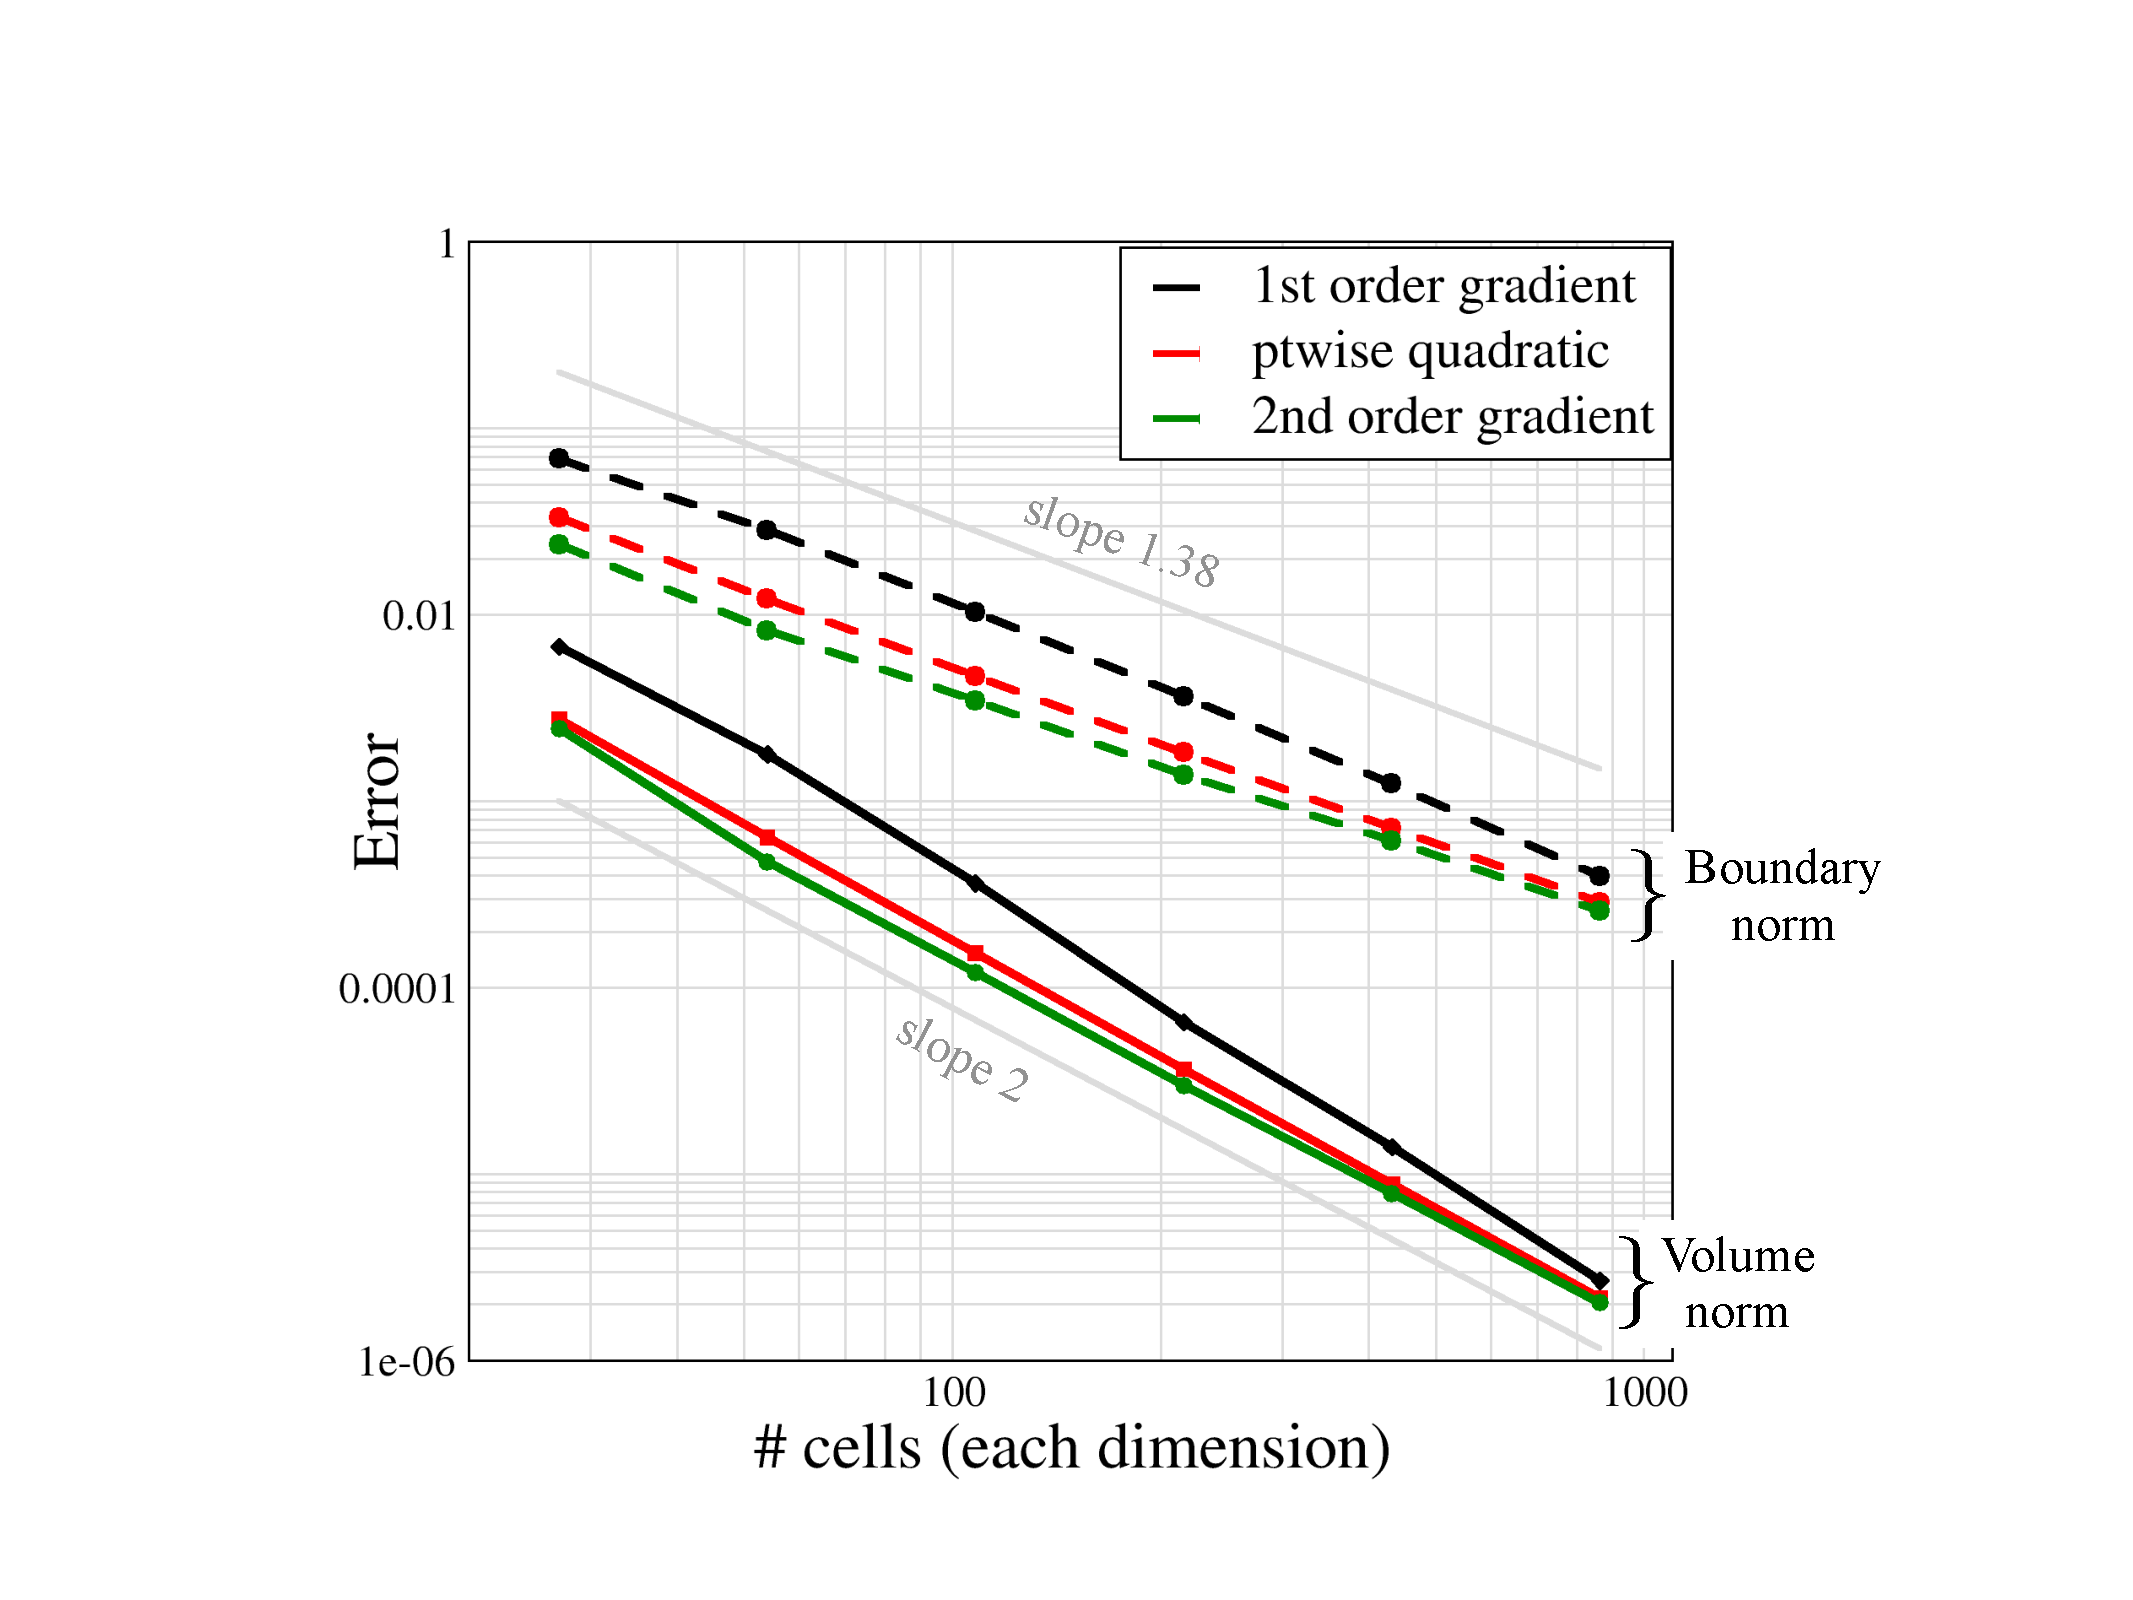
\includegraphics[height=3.0in]{figs/gradientConv.pdf}
		\caption{\sf Convergence in the L1 norm of the error in the entire 
			domain  (solid line), and along the boundary (dashed line).
			The reference line has slope 2 next to the domain error. The convergence
			rate at the boundary is between 1.38 and 1.5
			along the boundary.
			\label{fig:ssv}}
	\end{center}
\end{figure}


Note that the error at the cut cells is larger than in the volume, and has a
slower convergence rate. Since the number of cut cells grows only
linearly with refinement, the $L_1$
accuracy in the entire flow field is still second order.  At the boundary,
Richardson extrapolation shows that the convergence rate seems to be
between 1.38 and 1.5.
This has also been found in other cut cell studies \cite{KB:2006,nemec_tm14}, and 
is not due to SRD.

Figure \ref{fig:ssv} and Table \ref{tab:ssv}  show that using pointwise 
quadratic cut cell gradients is roughly
a factor of 2 more accurate on coarser grids.  The more complicated second order
acccurate gradient is even more accurate, especially on coarser grids.  Ultimately the gradient
error is reduced, and the error curves for the first and second order 
accurate gradients approach each other. 


We also use this example to compare the effect of state redistribution versus 
marching to steady state using local time-stepping without SRD.  
Table  \ref{tab:ssv2} shows a comparison of the error in the converged
solution using local time stepping (LTS)  without SRD, and the error with full timesteps and
SRD stabilization, both using  first order accurate gradients. 
The errors are essentially identical, showing that 
SRD does not degrade the computed solution with too much diffusion due
to the merging neighborhoods. This holds across all the other
gradient formulations too.


{
\small
\begin{table}[h]
\centering
 	\begin{tabular}{|l|c|l|l||l|l|} \hline
 		$h$ & $N_x ,N_y$ & \multicolumn{2}{|c|} {Volume Error} & \multicolumn{2}{|c|}{Boundary Error} \\ 
                \hline
 		    &            & {LTS (no SRD)} & SRD  & LTS (no SRD)  & SRD  \\ \hline
 			.5297 & 27 & 6.09e-3  &  6.75e-3   &  6.75e-02       &  6.84e-02 \\
 			\hline
 			.2648 & 54  & 1.67e-3  (3.6)  & 1.78e-4 (3.8)  &  2.79e-02  (2.4) &  2.83e-02 (2.4) \\
 			\hline
 			.1324 &108 & 3.41e-3  (4.9)  & 3.63e-4 (4.9)   &  1.00e-02  (2.8) &  1.03e-02  (2.8)\\
 			\hline
 			.662e-2 & 216 & 6.62e-5  (5.2)  & 6.52e-5 (5.6)  &  3.51e-03  (2.9) &  3.65e-03  (2.8)\\
 			\hline
 			.331e-2 & 432 & 1.34e-5  (4.9)  & 1.40e-5 (4.7)  &  1.21e-03  (2.9) &  1.24e-03  (3.0)  \\
 			\hline
 			.166e-2 & 864 & 2.59e-6  (5.2)  & 2.68e-6 (5.2)  &  3.78e-04  (3.2) &  3.96e-04  (3.1)  \\
 			\hline \hline
 	\end{tabular}
 	\caption{\sf Comparison of errors using local time stepping, which does not use SRD, 
        and regular time stepping with SRD. (The SRD errors are repeated here for easier
        comparison.) The errors are almost identical, except on the coarsest
        grid, showing that SRD does not 
        degrade the solution with too much diffusion. \label{tab:ssv2}}
\end{table}
}



\subsection{Shock Reflection from  Cylinder}
Next we demonstrate the method for the Euler equations using a Mach 2
shock diffracting around a circular cylinder. A cylinder with radius $0.15$ is centered at
(0.5,0.5), and the shock is initially located at $x = 0.2$.
For this example we compare results using the MUSCL scheme and
the Method of Lines as the base schemes, both using local Lax Friedrichs for the Riemann
solver. The BJ limiter is used to limit
both the base scheme irregular cells  and tile reconstruction gradients. 

Figure \ref{fig:cyl1} (left) shows the solution density from MUSCL, and
right from MOL, at time $t=0.25$. 
Both grids use 302 cells in each
directions, and the domain is  $[0.0,0.0,]$ by  $[1.00001, 1.0]$, again to
prevent mesh degeneracies.
There are 416 cut cells
around the cylinder; 160 of the cut cells had volume fractions less than
0.5 and were stabilized with SRD.  The smallest volume fraction was 1.17E-4.   
For comparison, this is also the time shown in \cite{mjb-hel-rjl:hbox2}. 
Here and in \cite{mjb-hel-rjl:hbox2}, the front of the cylinder where the
maximum density is found is better behaved with the one-step methods than with
MOL.  The method of lines solution is smoother around the boundary than our
MUSCL variant (see Figure \ref{fig:cylbndry}).

\begin{figure}[h]
\begin{center}
\vspace*{-.1in}
\hspace*{-.4in}
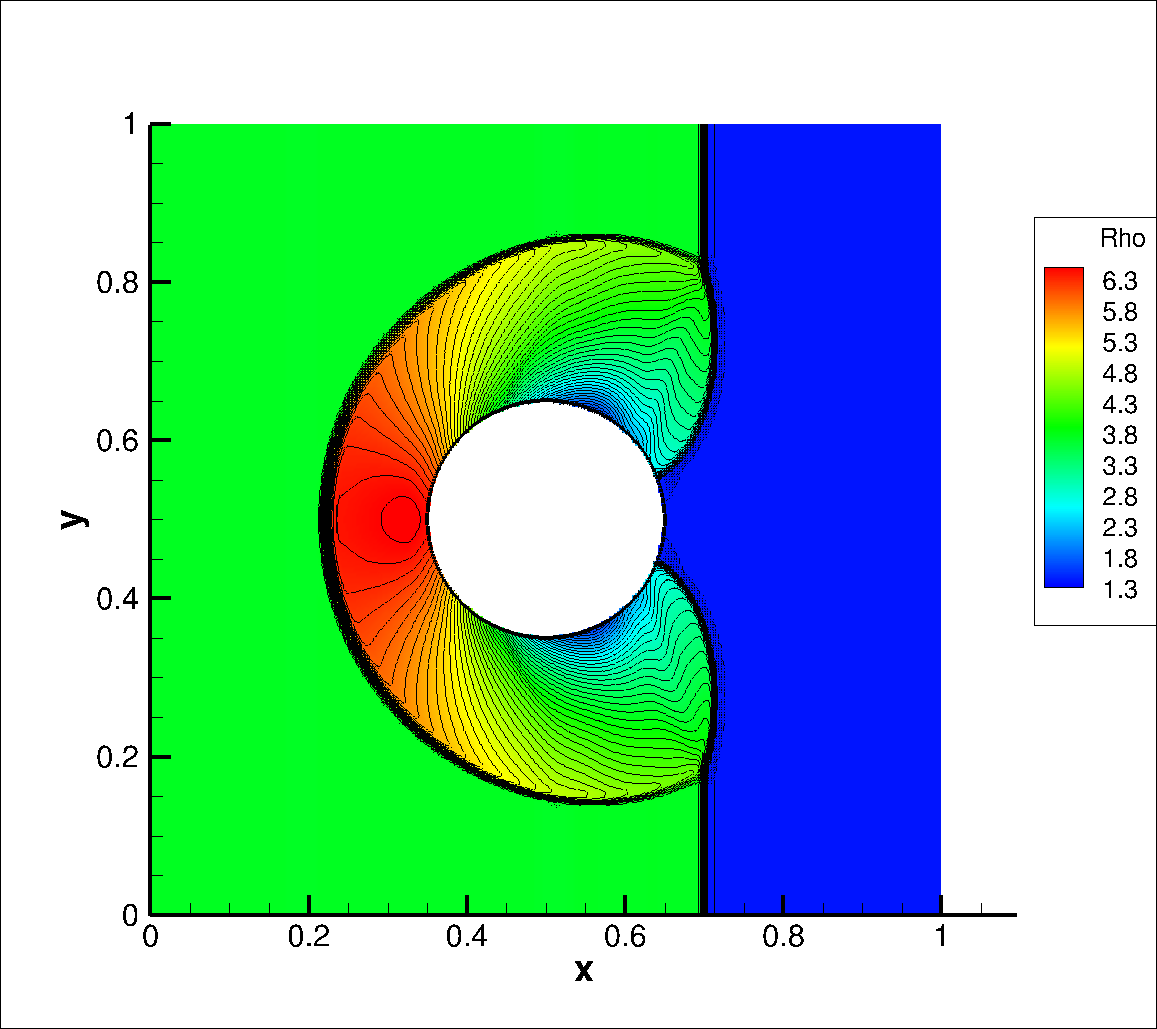
\includegraphics[width=0.48\linewidth,trim=10 10 200 10,clip]{figs/muscl_302cells.png}
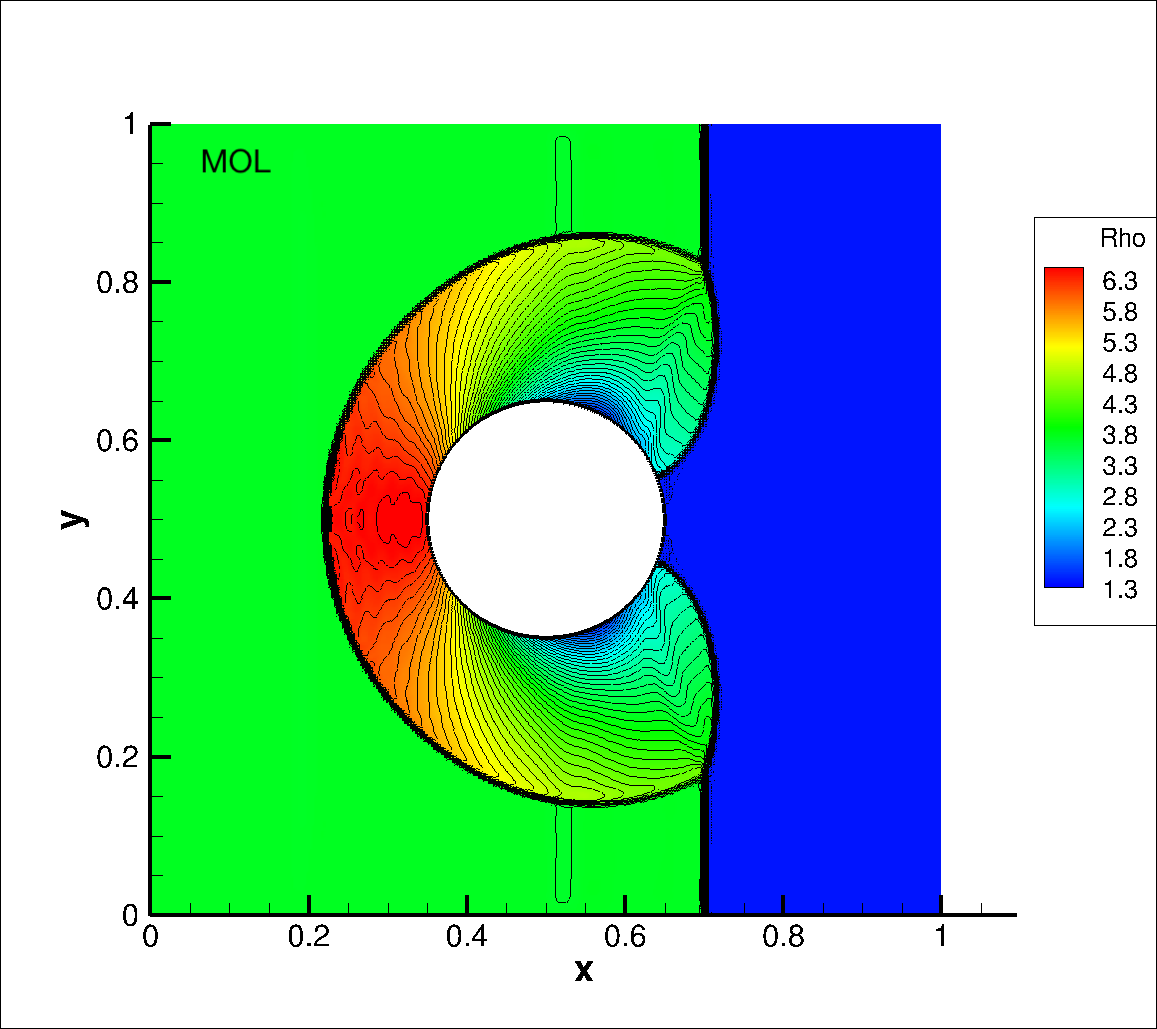
\includegraphics[width=0.48\linewidth,trim=10 10 200 10,clip]{figs/MOL_302cells.png}
\caption{\sf Density profile of Mach 2 shock reflection around a cylinder,
at time t=0.25.  Left computation used MUSCL, right used MOL. 
There are 52 contours between 1.3 and 6.5.
The front of the cylinder is better behaved with MUSCL, but the solution
at the cut cells is better  with the method of lines.
\label{fig:cyl1}}
\end{center}
\vspace*{-.1in}
\end{figure}

Figure \ref{fig:cylbndry}
shows the density profile from both schemes
taken along the cylinder.
For this plot, the cut cell variable is
reconstructed to the midpoint of the cylinder line segment in each  cell.  
The zoom shows the difference more
clearly.

\begin{figure}
\begin{center}
%\includegraphics[width=0.48\linewidth,trim=20 20 20 30,clip]{figs/densityCompare_302_normalvs3by3.png}
\hspace*{-.5in}
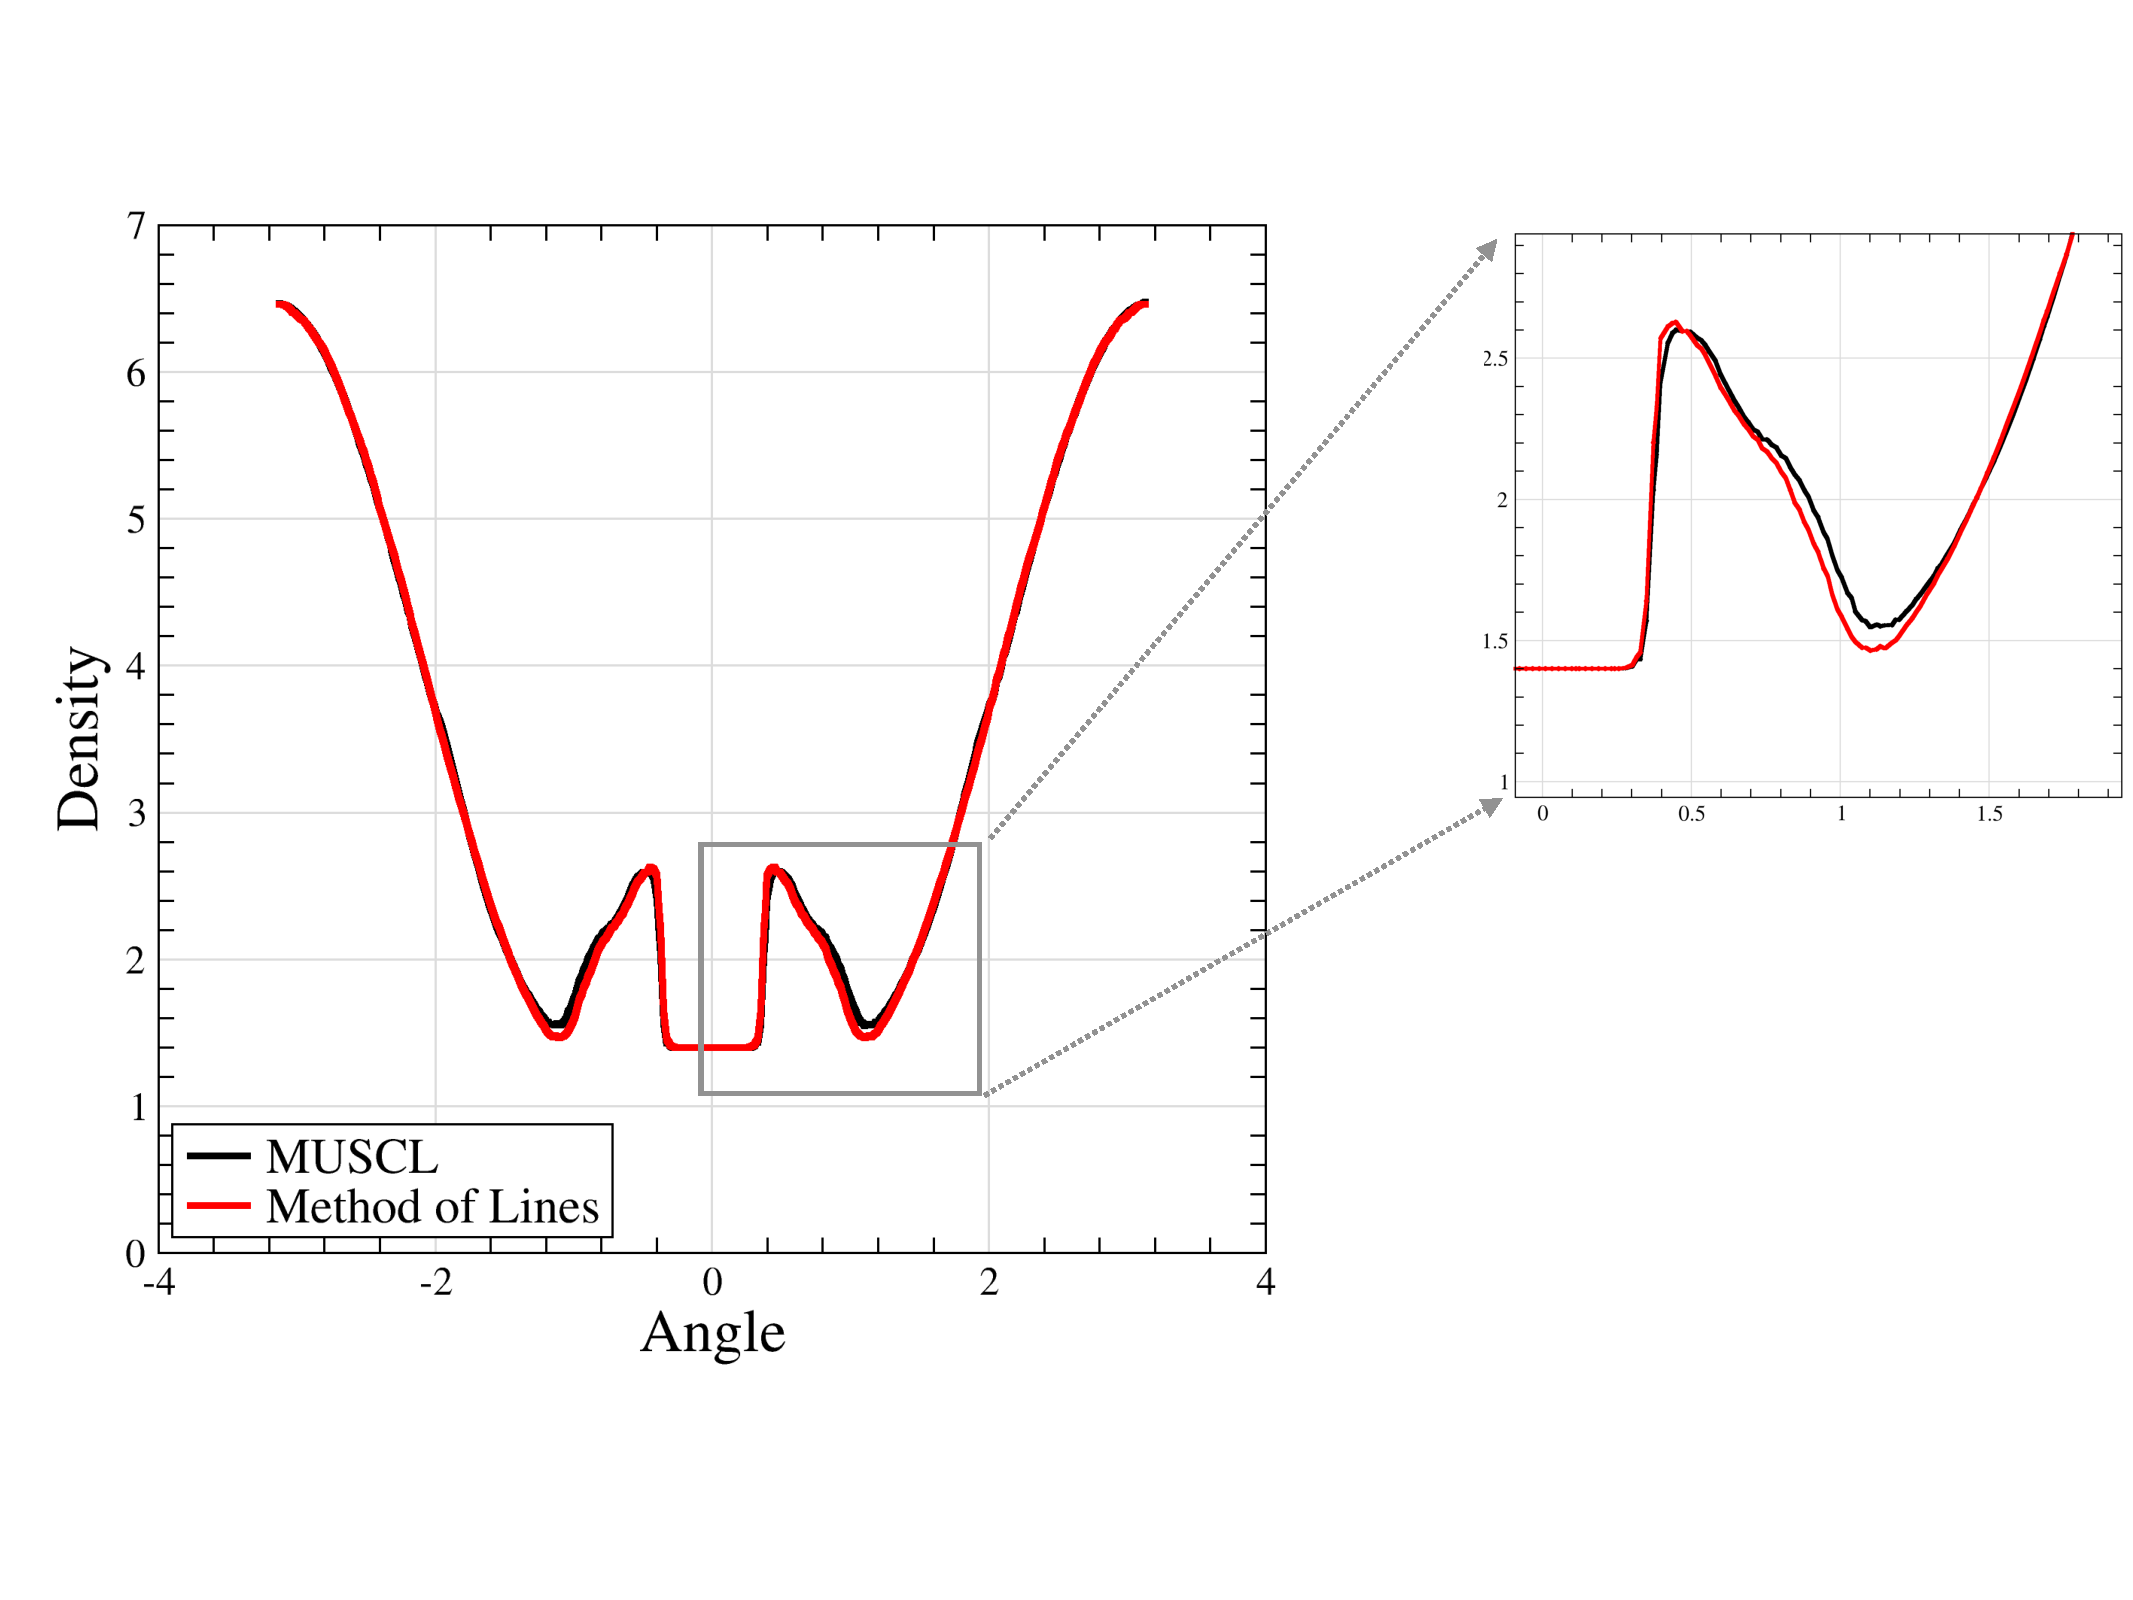
\includegraphics[height=2.7in]{figs/MM_densityBndry.pdf}
\hspace*{.3in}
%\includegraphics[width=0.48\linewidth,trim=20 20 20 30,clip]{figs/pressureCompare_302_normalvs3by3.png}
%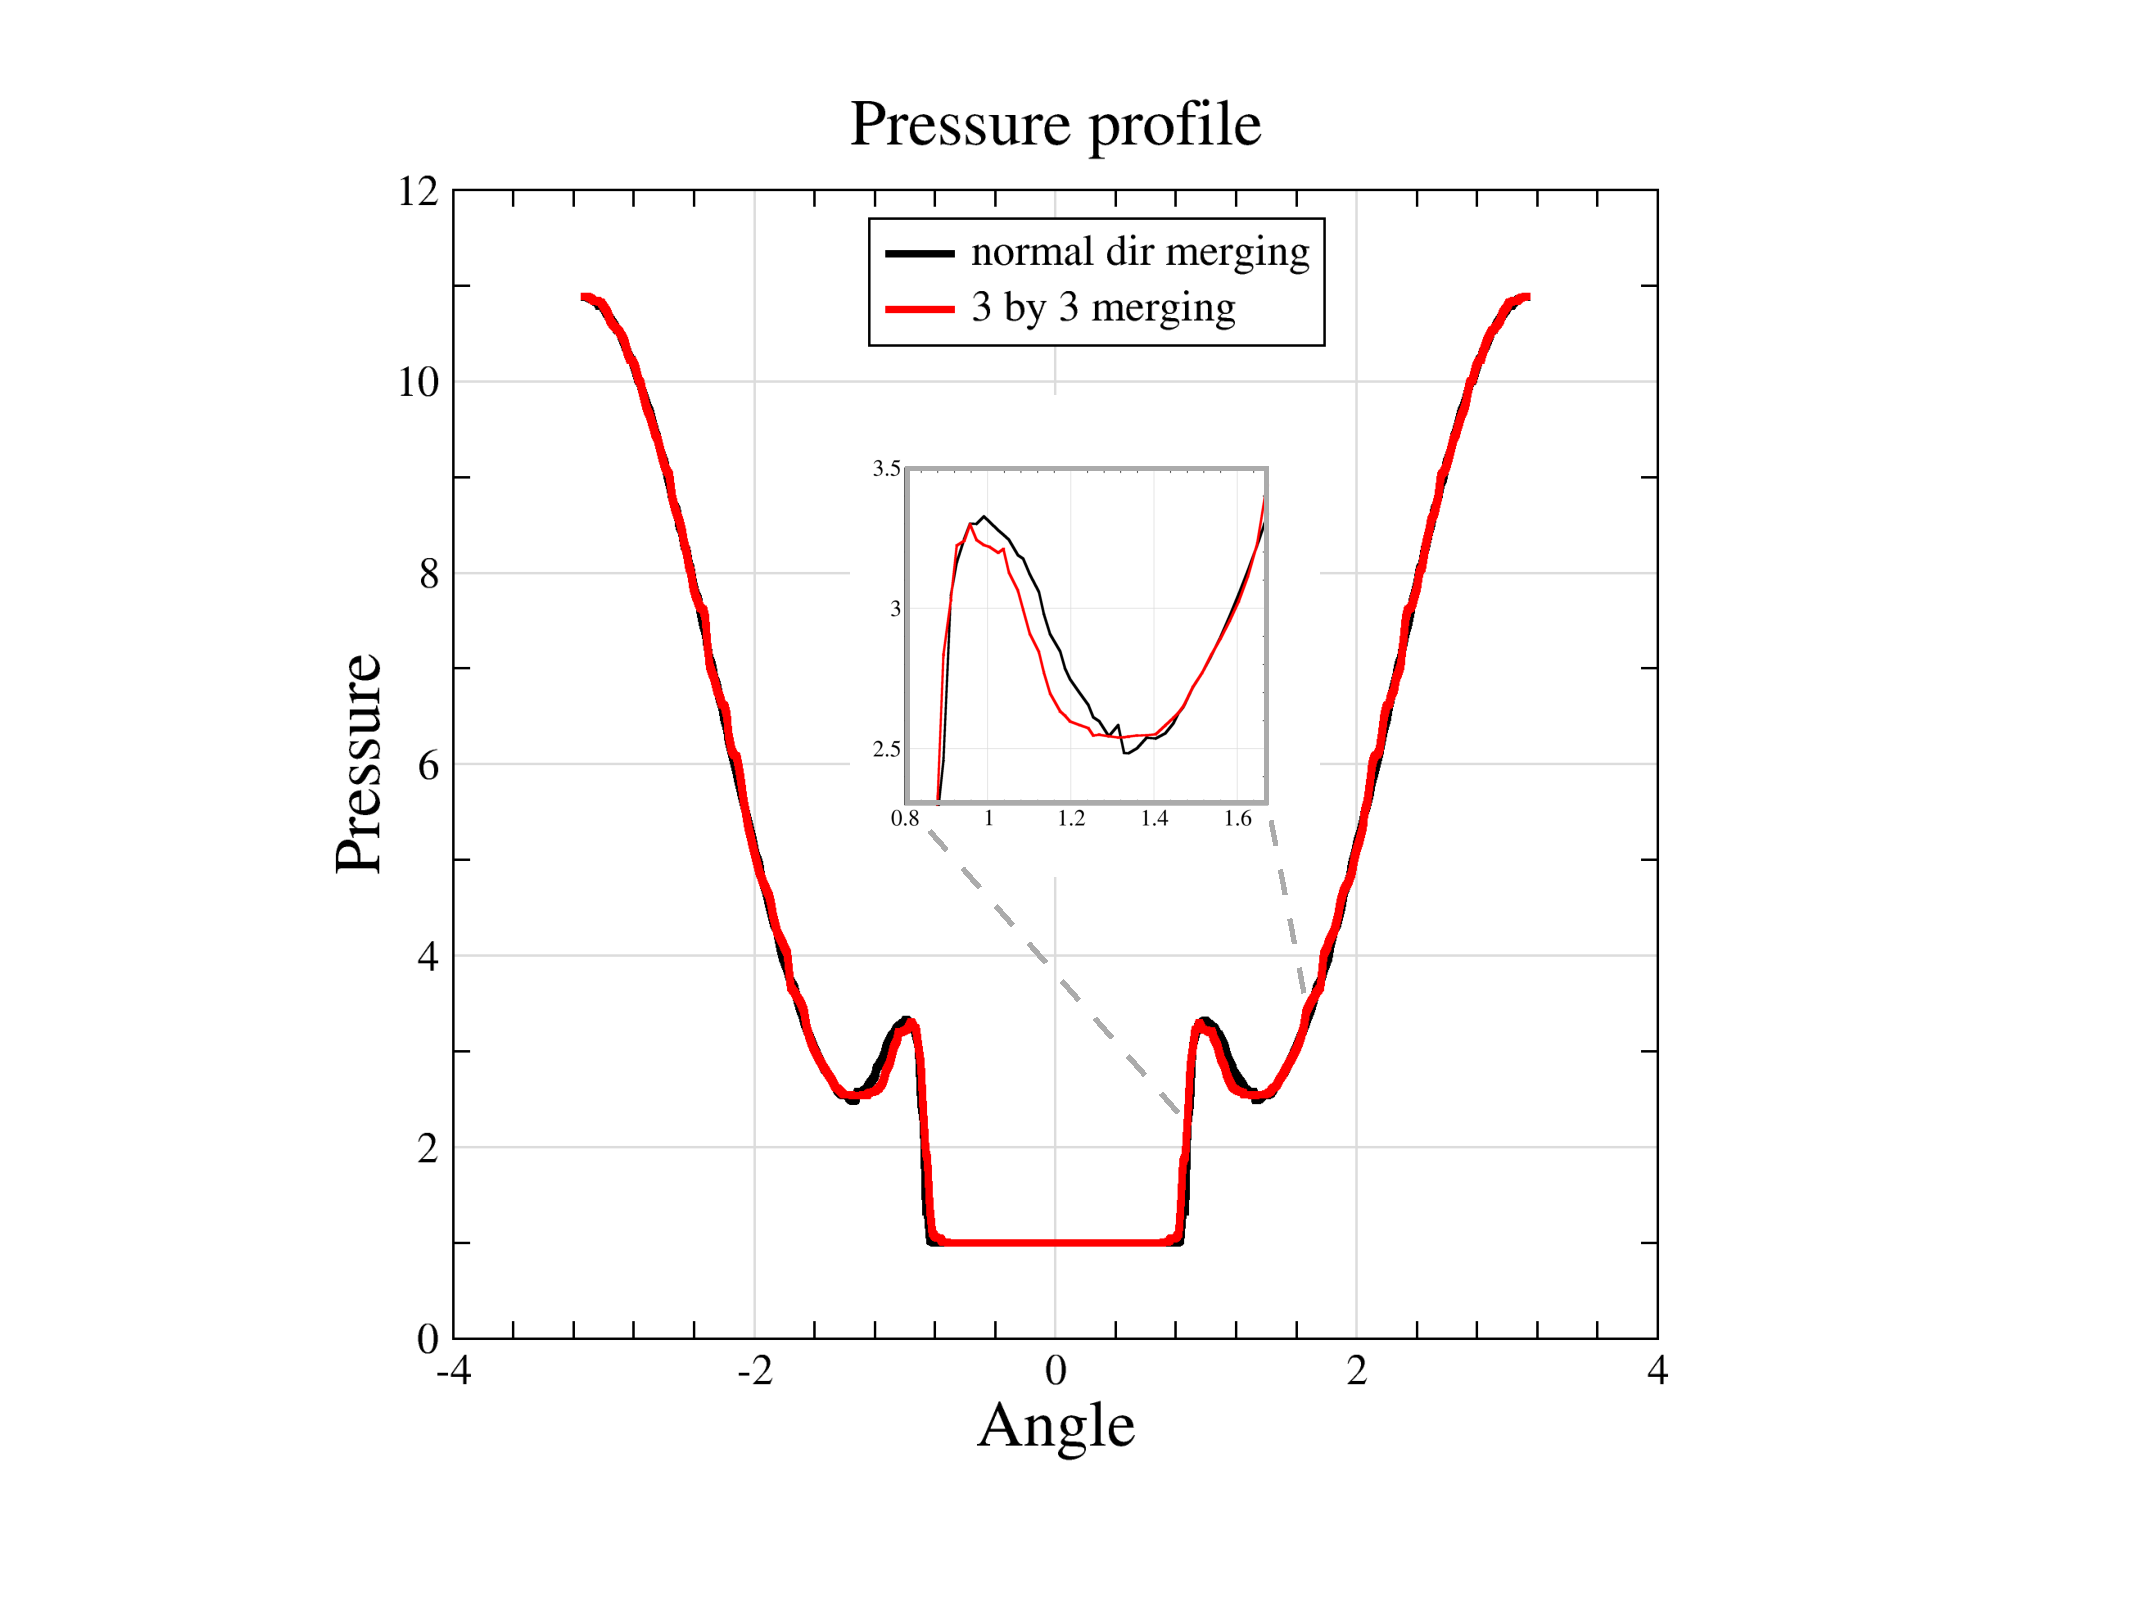
\includegraphics[height=2.7in,trim=120 70 230 50,clip]{figs/pressureWithZoom.pdf}
\caption{\sf The density profile  around the cylinder for the MUSCL and MOL schemes 
at time t=0.25.  The MOL scheme has smoother results.}
\label{fig:cylbndry}
\end{center}
% fig in amrclaw-amrcart/example/cylinder_Mach2 directory on juniper
% using sortedcyl.dat (coied from bndry01.dat) in the various _output dirs
\end{figure}

\clearpage

\subsection{Double Mach Reflection problem}\label{sec:dm}
In this section, we reflect a Mach 10 shock obliquely over a wedge, 
where the shock and wall form a $60^{\circ}$ angle.  
The problem domain is $[0,3.0]\times[0,1.75]$, with an angled wall 
passing through the point $(1/6,0)$ . The ramp is outlined in red in Figure
\ref{fig:dm}.
We use the finite volume MUSCL scheme with second order slopes on the base 
grid and SRD neighborhoods, and limit using Barth Jespersen.
The solution to this problem is a complex, self-similar reflection pattern 
composed of incident and reflected shocks, Mach stem, and a contact 
discontinuity \cite{WOODWARD1984115,rkdg5}.  
The contact discontinuity is an unstable feature of the solution that can be 
difficult to resolve correctly, especially in the neighborhood of the 
reflecting boundary where the carbuncle phenomenon can occur \cite{KEMM2018596}.

\begin{figure}[h]
\centering
%\includegraphics[width=0.48\linewidth]{figs/doublemach.png}
%\includegraphics[width=0.48\linewidth]{figs/doublemach_zoom.png}
%\includegraphics[width=1.1\linewidth]{figs/doubleMach.pdf}
\hspace*{-.25in}
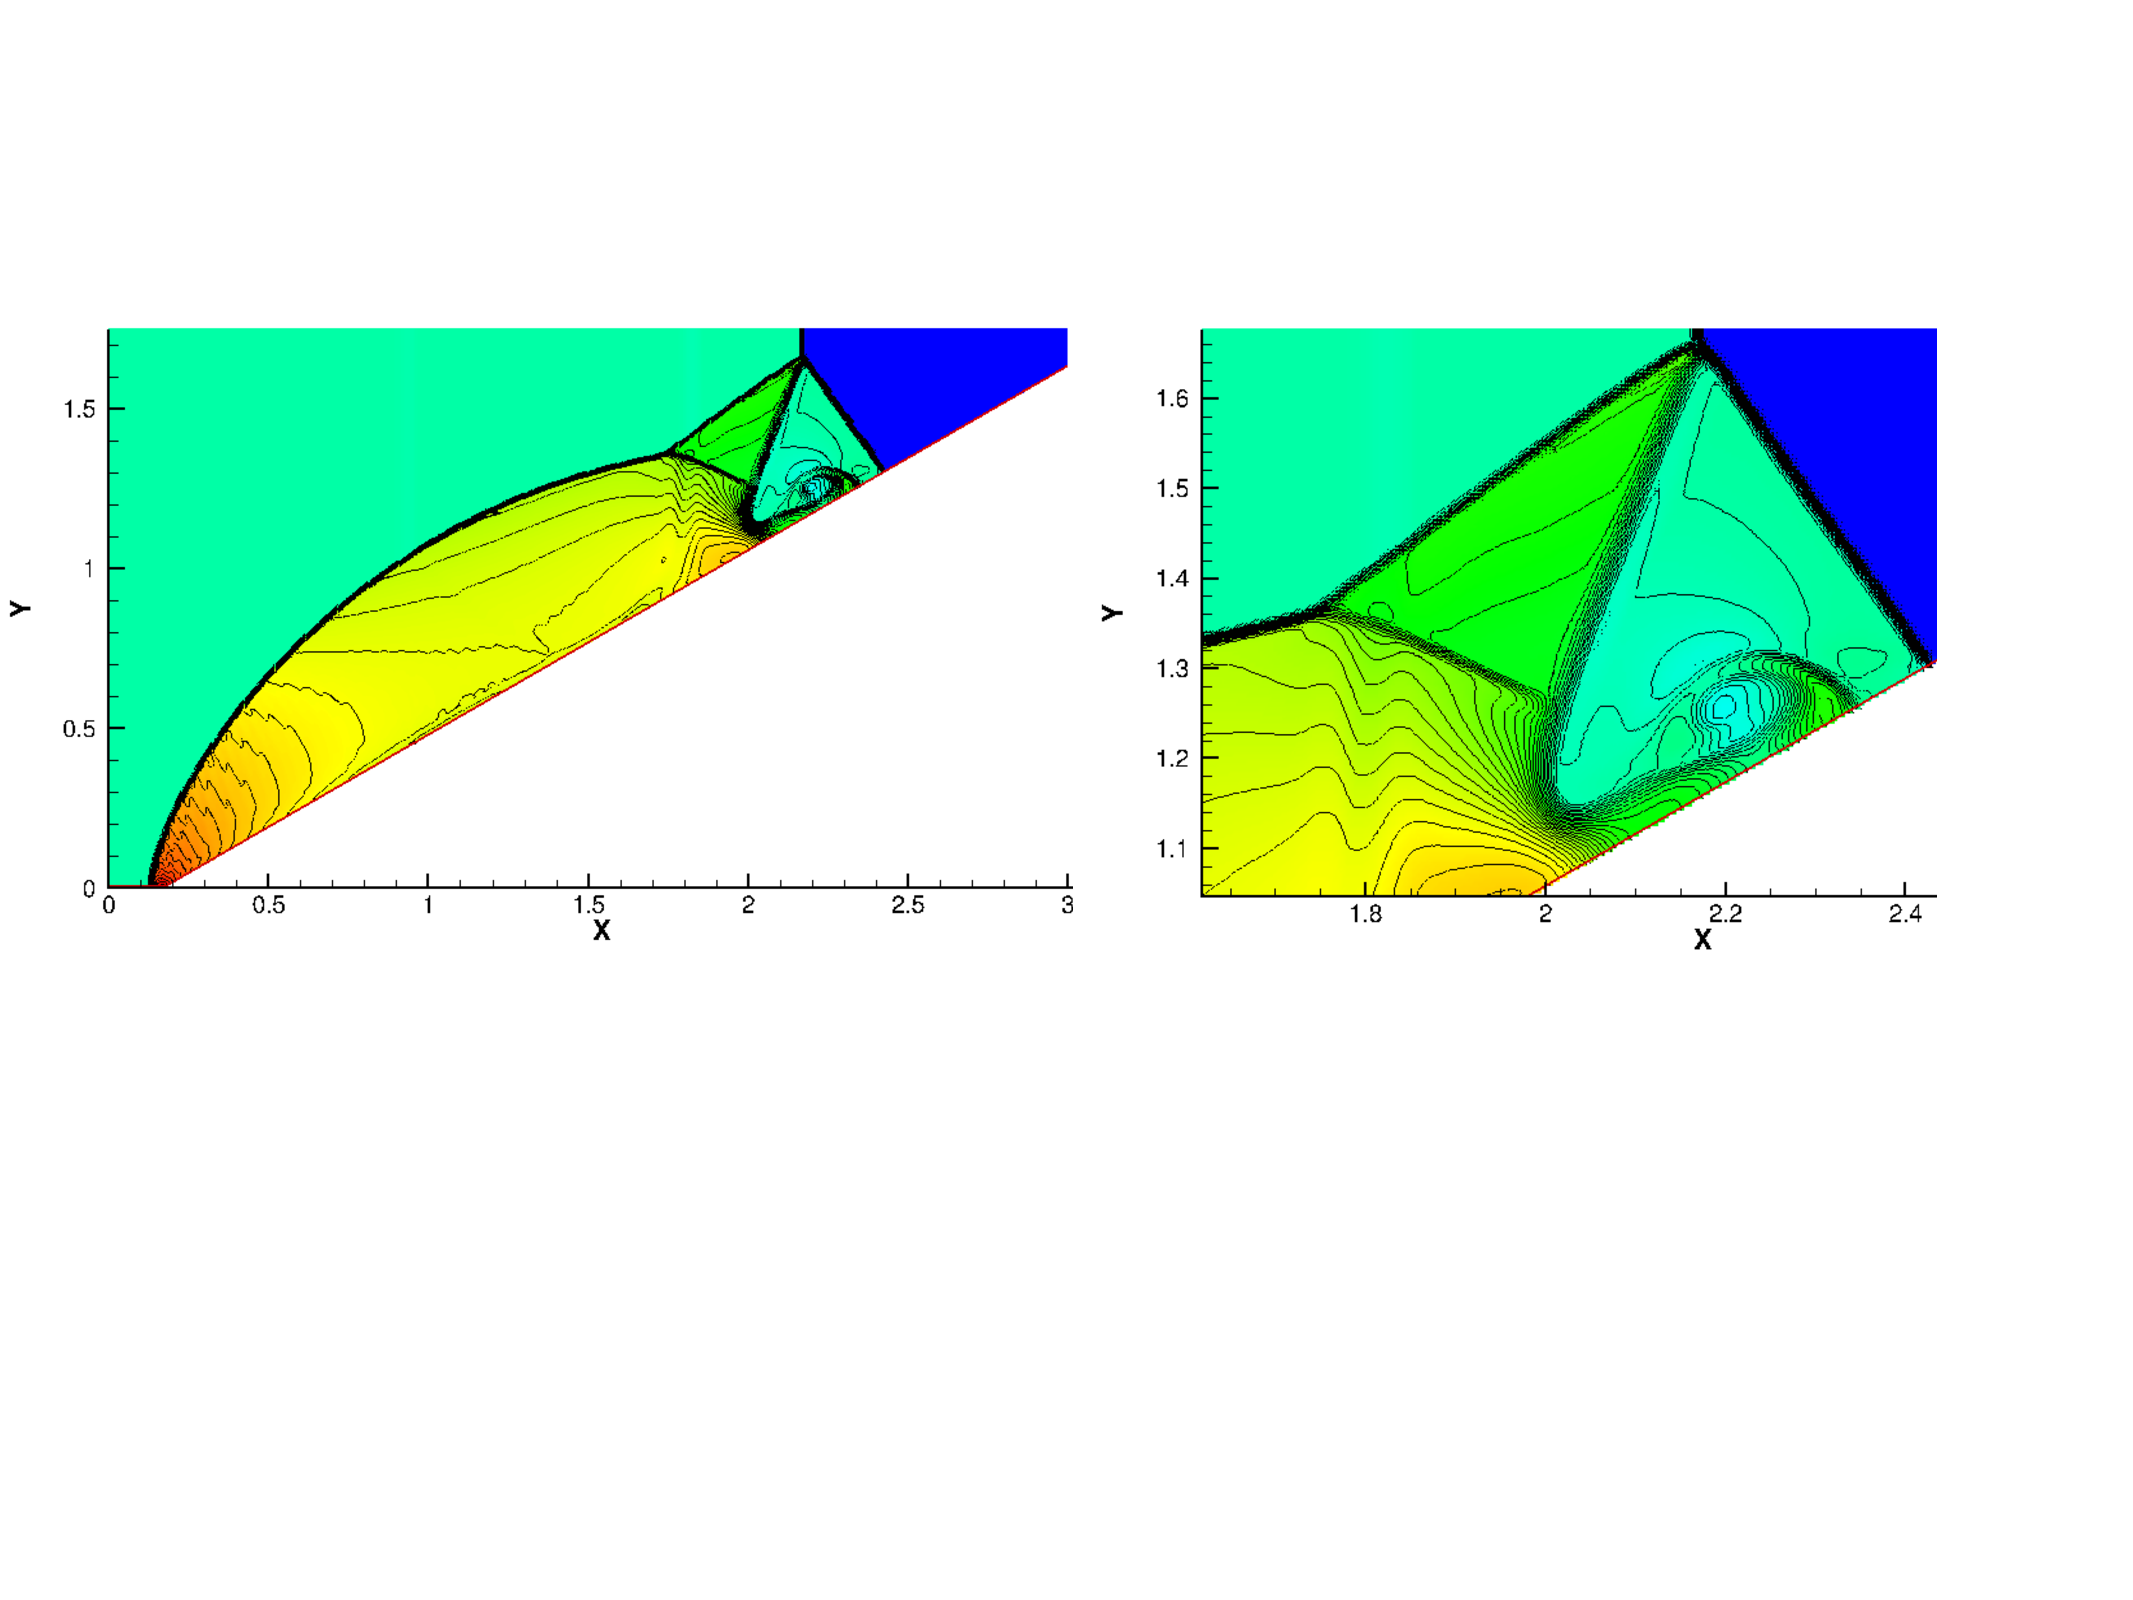
\includegraphics[width=1.1\linewidth]{figs/doubleMach240.pdf}
\hspace*{-.25in}
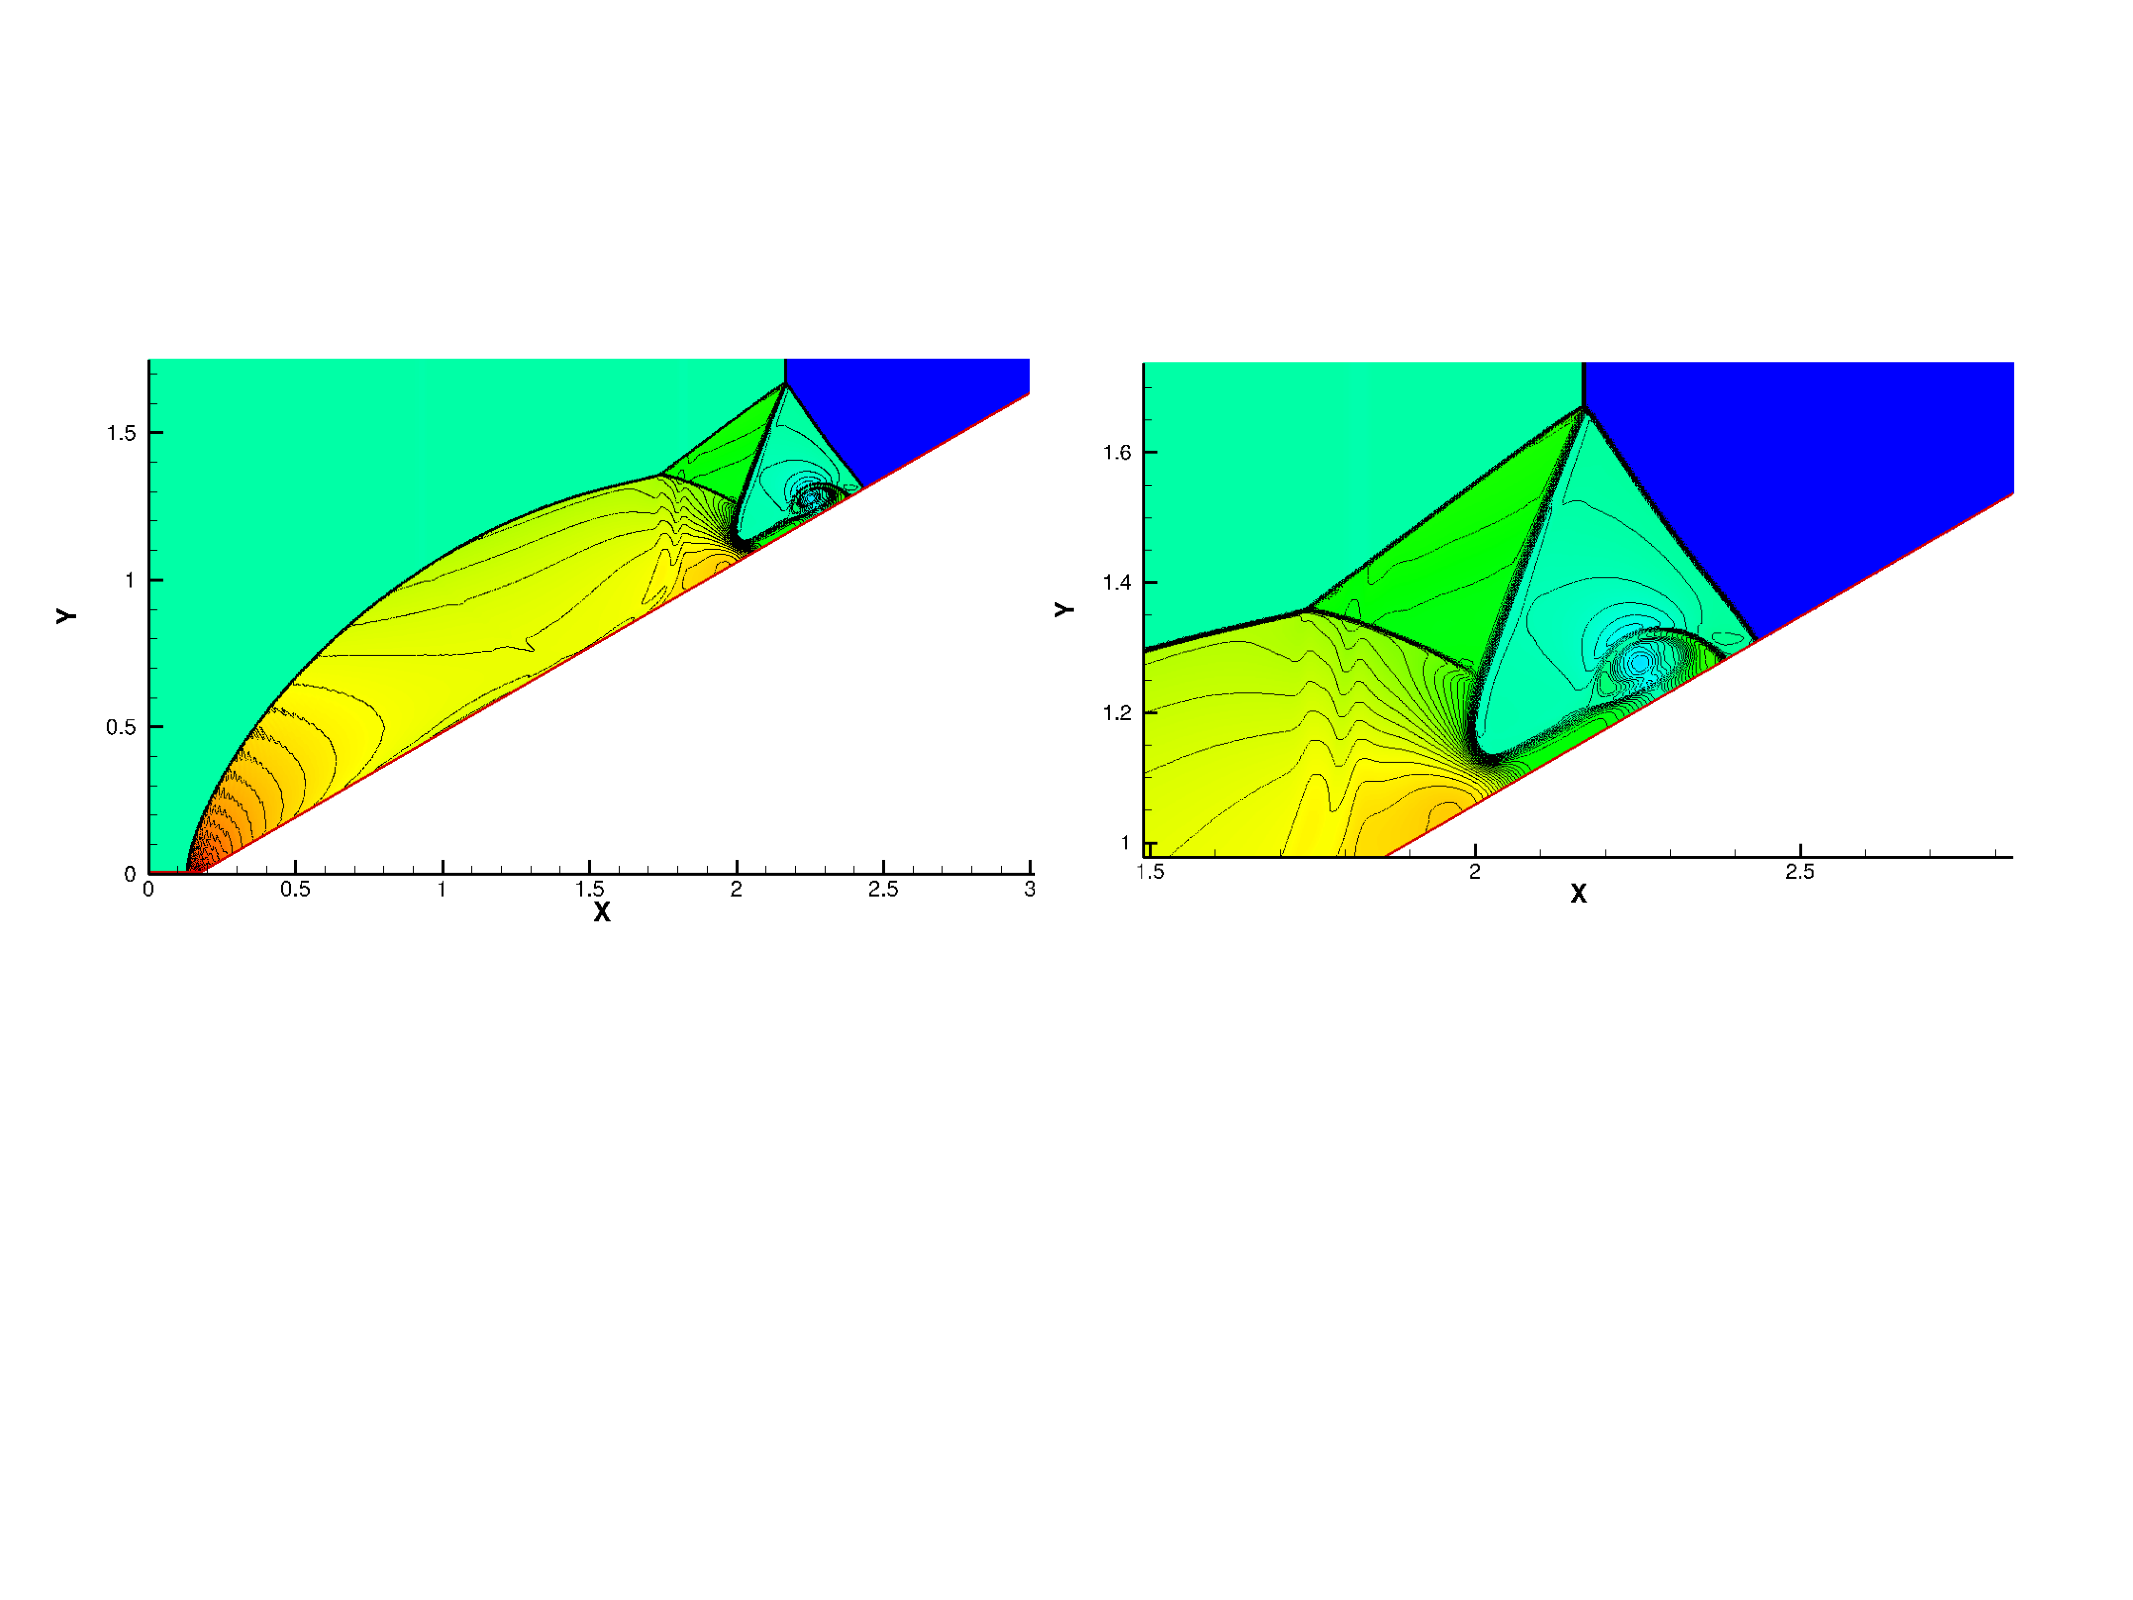
\includegraphics[width=1.1\linewidth]{figs/doubleMach480.pdf}
\caption{\sf Density plot and isolines of a Mach 10 shock impinging 
obliquely on a wedge at time $t = 0.2$ where $\Delta x = \Delta y =
1/240$ (top) and 1/480 (bottom).
The solution on the full domain is shown adjacent to a zoom of the Mach 
stem region.  Sixty isolines between 1.39 and 21.0 are drawn.}\label{fig:dm}
\end{figure}

The solution at the final time $T = 0.2$ is plotted in Figure \ref{fig:dm}, 
where the grid resolution is $\Delta x = \Delta y = 1/240$.
We obtain qualitatively comparable results to those in \cite{rkdg5} on 
the same grid resolution. We also show for comparison the results using 
$\Delta x = \Delta y = 1/480$, also done in \cite{rkdg5}. Again, the
improvement is very similar. Finally, in Figure \ref{fig:wedgeBndry} we
show the density along the boundary for the two resolutions. Despite the
irregularity of the cut cells, the solution is very smooth. The smallest
cut cell in the coarser grid has volume fraction 1.65e-6. On the finest
grid the smallest volume fraction is 2.95e-7. 

\begin{figure}[h]
\centering
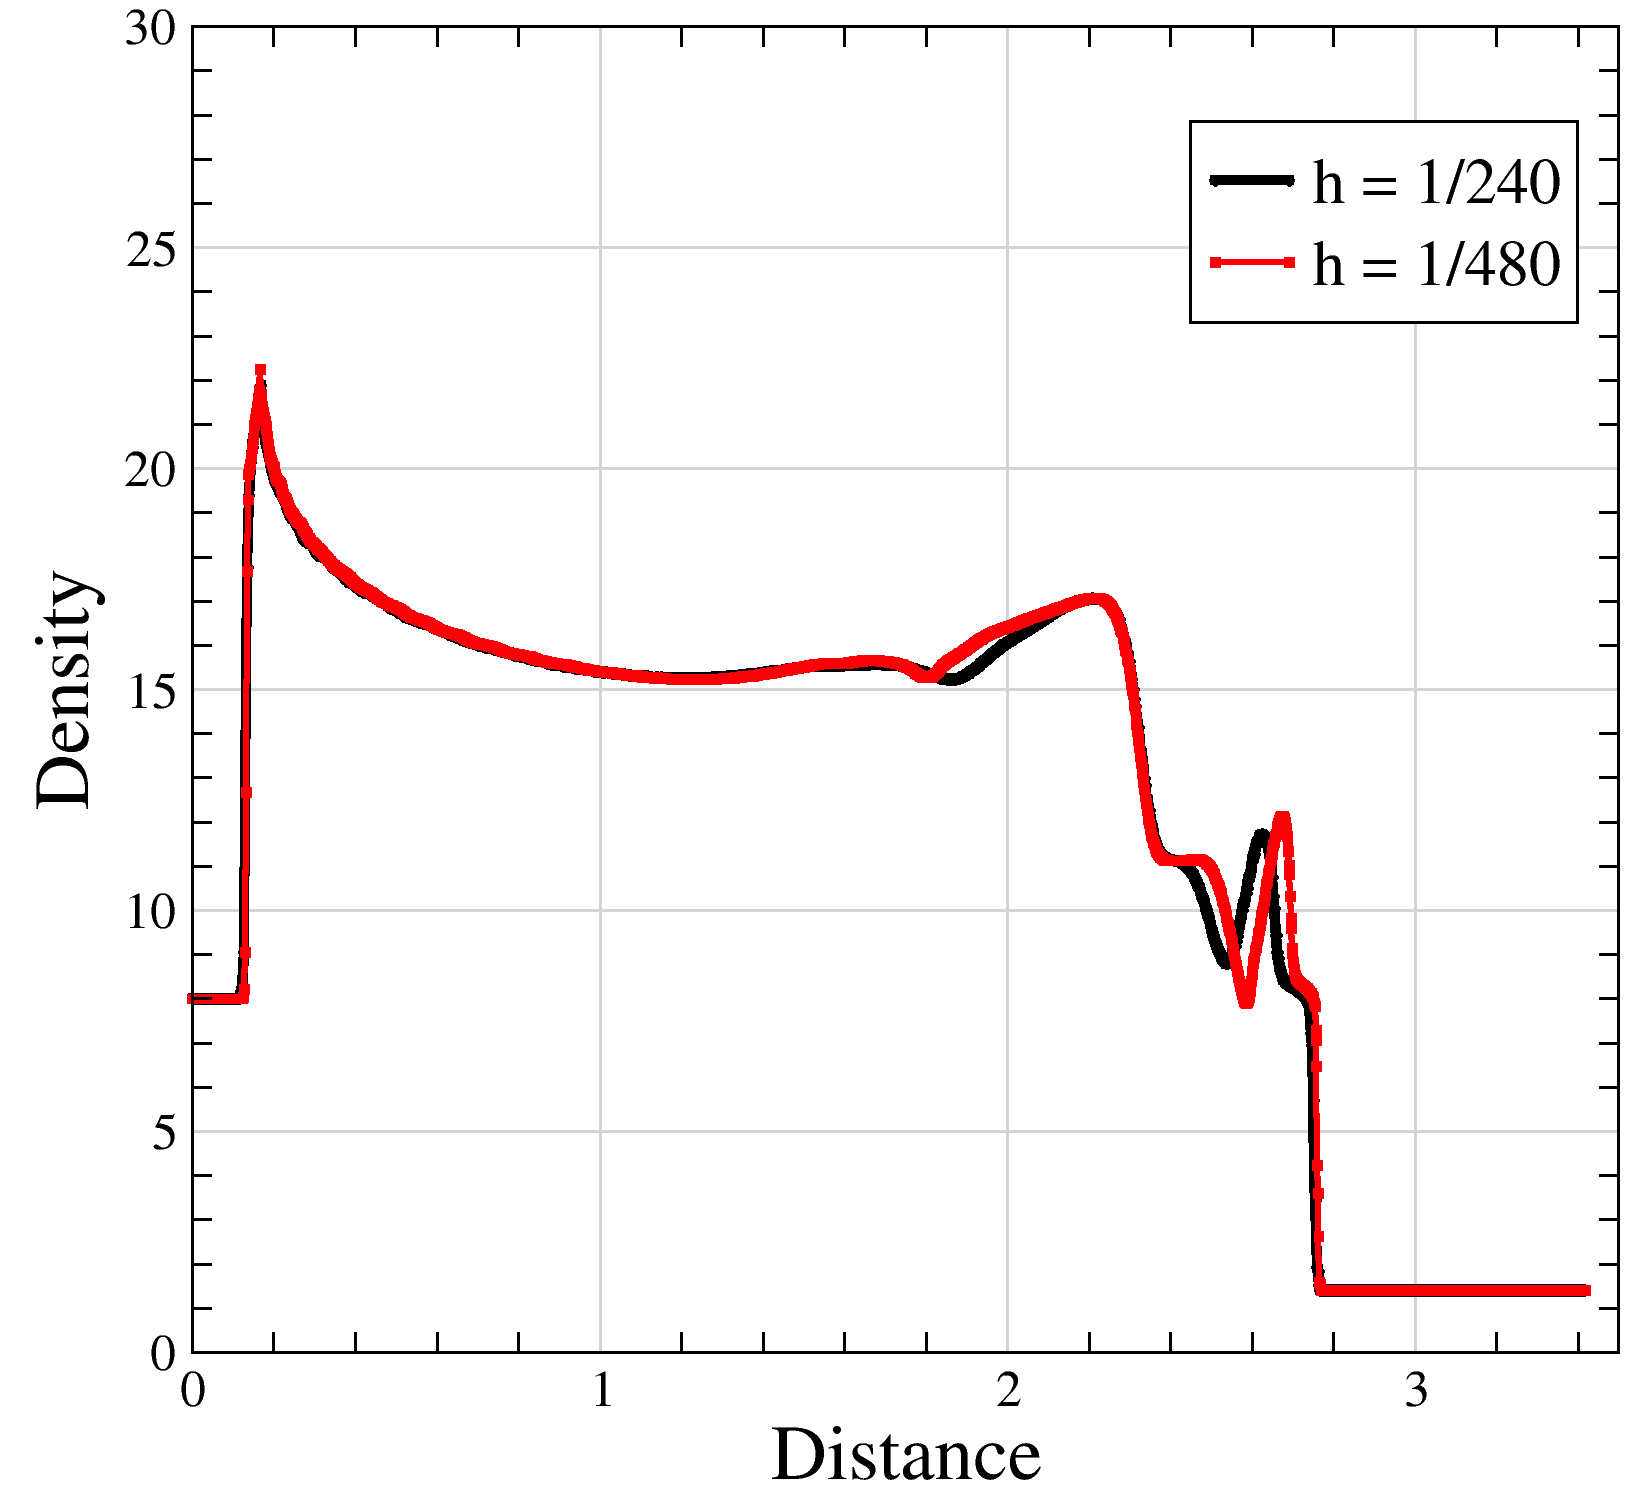
\includegraphics[width=.7\linewidth]{figs/rampWall.png}
\caption{\sf Density plotted along the wall, as a function of distance from
the lower left corner of the domain. The coarser grid has a bit of
oscillation after the ramp starts due to the curved shock. It is not due to
SRD. It is not present on the finer grid .} \label{fig:wedgeBndry}
\end{figure}



\section{Conclusions}\label{sec:conc}
We have presented a  state redistribution algorithm to solve the small cell problem on cut cell meshes.  It is conservative, allows for overlapping temporary merging neighborhoods so is easy to implement, and is linearity preserving.   
Numerical experiments show that on smooth problems, second order accuracy is maintained, and the solution is not degraded by the postprocessing. For problems with shocks, the scheme maintains robustness at the cut cells.
We have shown experiments using SRD on two different base schemes, but it should be 
applicable to any underlying numerical method with
cell-centered variables.

We think that state redistribution should be applicable to 
different sets of equations, and to three-dimensional applications.
It also seems clear that the scheme can be extended to higher order accuracy, 
when used in conjunction with a 
higher order base scheme. We have already started extending this work to
3rd and 4th order accuracy. Higher order methods bring 
in many new features however, so we do not include that here.

\appendix
\section{High order accurate base scheme}\label{sec:ho}
This section provides a framework to extend the method of lines finite volume scheme to high order.  
%The high order state redistribution could also be applied to a high order MUSCL scheme but we do not do this here.  
In Section \ref{sec:ho_basescheme}, we describe the high order method of lines scheme.  This base scheme requires a high order polynomial reconstruction on each cell of the base grid described in Sections \ref{sec:ho_reconstruction} and \ref{sec:ho_reconstruction_primitive}.


\subsection{Method of lines} \label{sec:ho_basescheme}


High order accuracy in space is achieved by reconstructing a high order polynomial on each cell and using it to evaluate the numerical flux at the face quadrature points (Figure \ref{fig:2dfig}).  
For third and fourth order accurate schemes, we use the two-point Gauss
Legendre quadrature rule illustrated by squares in Figure \ref{fig:2dfig_ho_vquad}.  Our
numerical experiments again use the local Lax-Friedrichs flux function.

The high order method of lines scheme requires quadrature rules on volumes for 
\begin{enumerate}
	\item the computation of cell averages for the initial condition $\mathbf{U}^0$,
	\item geometrical constants used in polynomial reconstruction (Sections \ref{sec:ho_reconstruction} and \ref{sec:ho_reconstruction_q}),
	\item reconstruction in primitive variables (Section \ref{sec:ho_reconstruction_primitive}).
\end{enumerate}

On cut cells, integrals are computed by first triangulating the cut cell, then using a quadrature rule of sufficient order on each subtriangle.  The triangulation is not necessarily Delaunay and we do not introduce new vertices to triangulate the cut cells.  This approach can result in thin and small triangles on the cut cell (Figure \ref{fig:2dfig_ho_vquad}).  It is simple to show that the accuracy of volume integrals approximated in this manner on cut cells will not be affected \cite{QIN201324}.
On full cells, we use quadrature rules designed for quadrilaterals.  

\begin{figure}
	\begin{center}
		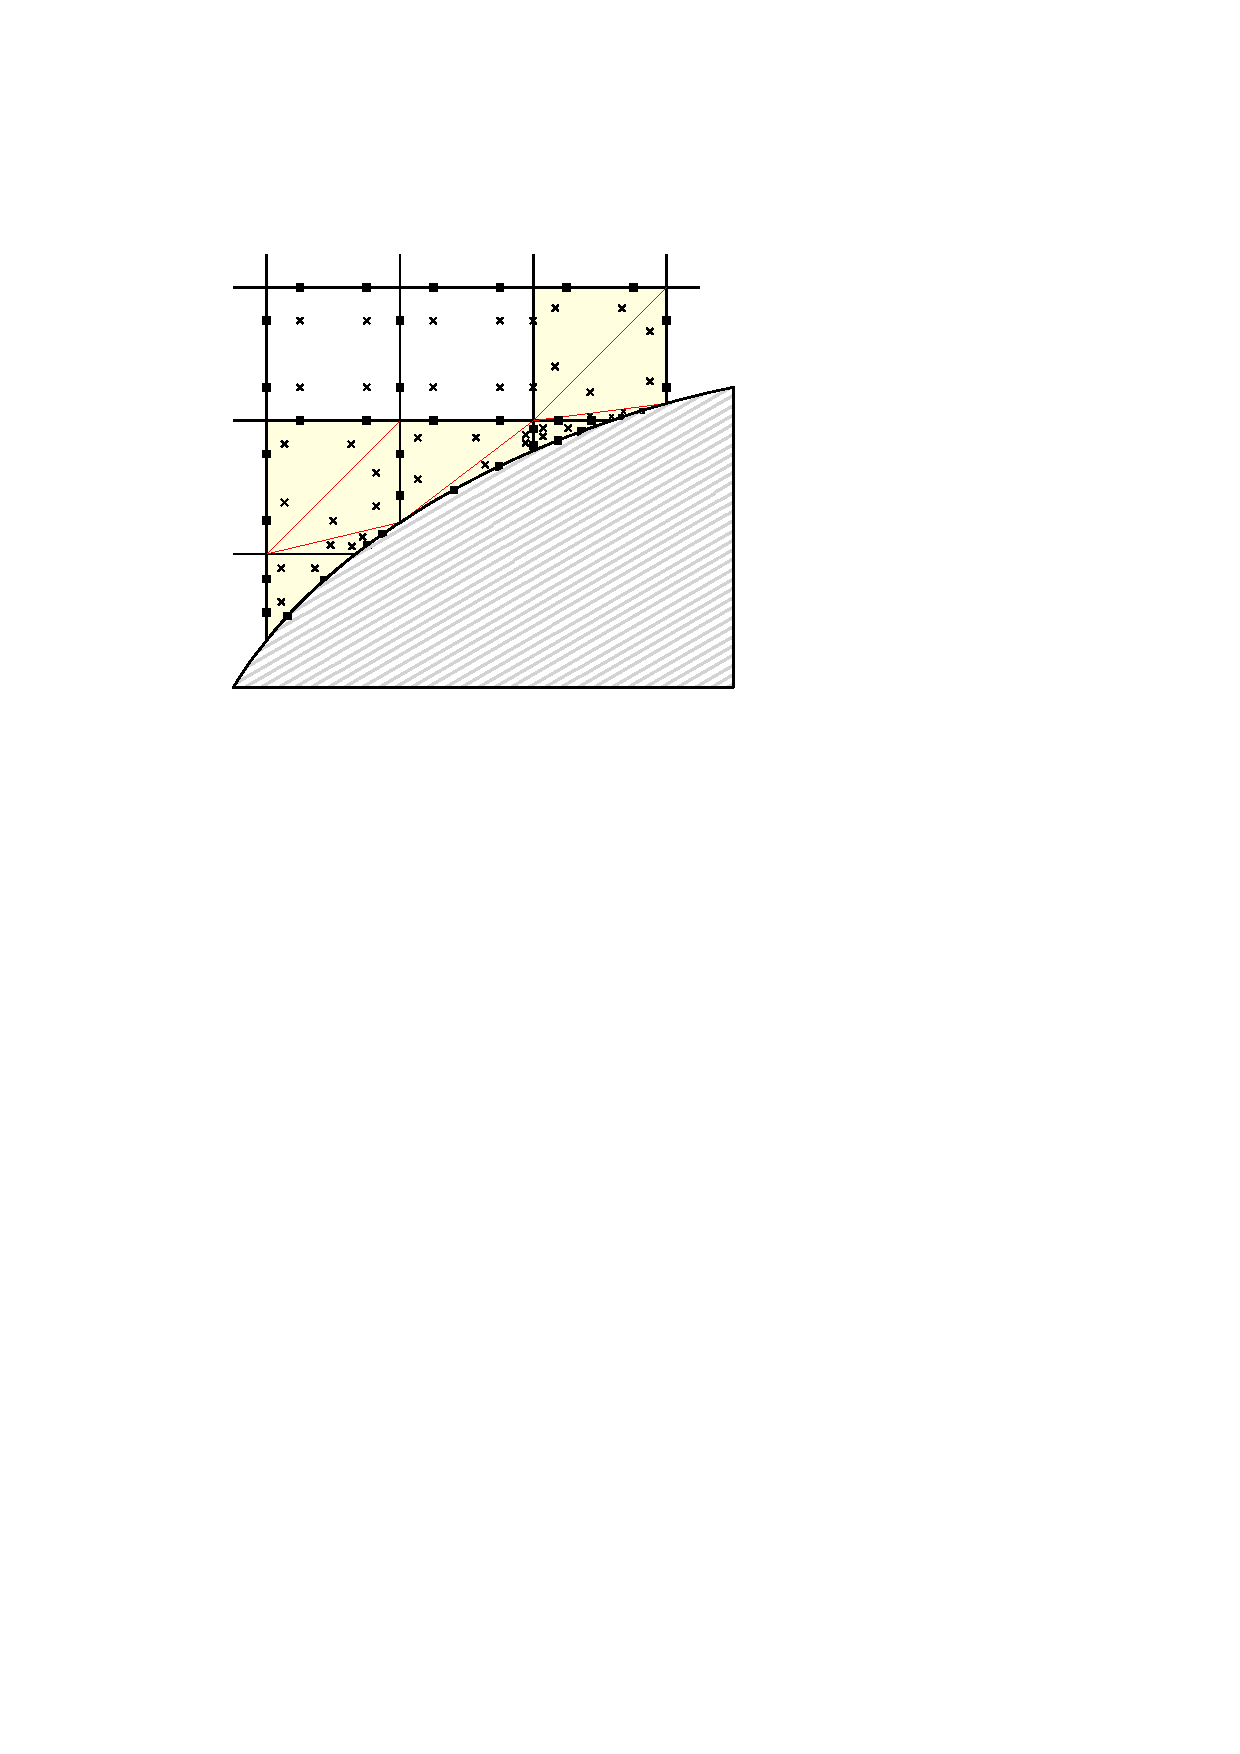
\includegraphics[width=3.0in]{figs/example_ccmesh_ho_vquad.pdf}
		\caption{\sf 
%			The high order method of lines scheme reconstructs to Gauss-Legendre quadrature points. 
			The two-point Gauss-Legendre quadrature points used for third and fourth order methods are indicated by a square ($\blacksquare$).  The triangulations used for volume integration on cut cells are indicated by red lines and the volume quadrature points for third and fourth order methods are indicated by a cross ($\times$).} 
		\label{fig:2dfig_ho_vquad}
	\end{center}
\end{figure}


High order accuracy in time is obtained by applying a Runge-Kutta method   
with the same degree accuracy in time  as the spatial reconstruction.
%We use the two stage TVD-RK2 scheme in \eqref{eq:molscheme} with linear reconstructions and the time step restriction given in \eqref{eq:vn1}.
For the third order method, we use the three stage TVD-RK3 method
%\begin{equation}\label{eq:molscheme_ho2}
%\begin{aligned}
%\mathbf{U}^{(1)} &= \mathbf{U}^{n} + \Delta t L(\mathbf{U}^n), \\
%\mathbf{U}^{(2)} &=  \frac{3}{4}\mathbf{U}^{n} + \frac{1}{4}(\mathbf{U}^{(1)} + \Delta t L(\mathbf{U}^{(1)})), \\
%\mathbf{U}^{(3)} &= \mathbf{U}^{(2)} + \Delta t L(\mathbf{U}^{(2)}),  \\
%\mathbf{U}^{n+1} &= \frac{1}{3}\mathbf{U}^{n} + \frac{2}{3}\mathbf{U}^{(3)}  ,	
%\end{aligned}
%\end{equation}
with the time step restriction
\begin{equation}
\Delta t \left( \frac{|a|}{\Delta x} + \frac{|b|}{\Delta y} \right) \leq 1.6,
\end{equation}
where $(a,b)$ are the wave speeds.
Note that this L2 stability limit is larger the SSP limit.
For the fourth order method, we use the standard four stage Runge-Kutta
scheme.
%since a four-stage TVD\_RK4 scheme does not exist..
%\begin{equation}\label{eq:molscheme_ho4}
%\begin{aligned}
%\mathbf{k}^{(1)} &= \Delta t L(\mathbf{U}^n), \\
%\mathbf{k}^{(2)} &= \Delta t L \left(\mathbf{U}^n + \frac{\Delta t}{2} \mathbf{k}^{(1)} \right), \\	
%\mathbf{k}^{(3)} &= \Delta t L \left(\mathbf{U}^n + \frac{\Delta t}{2} \mathbf{k}^{(2)} \right), \\	
%\mathbf{k}^{(4)} &= \Delta t L \left(\mathbf{U}^n + \Delta t \mathbf{k}^{(3)} \right), \\	
%\mathbf{U}^{n+1} &=\mathbf{U}^n + \frac{1}{6}(\mathbf{k}^{(1)} + \mathbf{k}^{(2)}+ \mathbf{k}^{(3)}+ \mathbf{k}^{(4)}),
%\end{aligned}
%\end{equation}
%and the time step restriction
%\begin{equation}
%\Delta t \left( \frac{|a|}{\Delta x} + \frac{|b|}{\Delta y} \right) \leq 1.2.
%%\end{equation}
%For both third and fourth order accurate methods, we have obtained their associated time step restrictions by numerical evaluation of the amplification factor resulting from a linear stability analysis.
%since a four-stage TVD-RK4 scheme does not exist
%\begin{figure}
%	\begin{center}
%		\includegraphics[width=3.0in]{figs/example_ccmesh_ho.pdf}
%		\caption{\sf Example base grid in two space dimensions. The cells shaded in yellow are the cut cells. The high order method of lines scheme reconstructs to Gauss-Legendre quadrature points.  We have indicated by the hollow cross ($\square$) the two-point Gauss-Legendre quadrature points used for reconstructions of degree $d=2,3$.} 
%		\label{fig:2dfig_ho}
%	\end{center}
%\end{figure}
%For these schemes, we use the following time step restriction
%\begin{equation}
%\Delta t   \max_{i,j}\left( \frac{|a_{i,j}|}{\Delta x} + \frac{|b_{i,j}|}{\Delta y} \right) \leq 1.
%\end{equation}


%It has been proven that this approach does not affect the accuracy

%In what follows, volume integrals are computed with quadrature rules of order $p$, when the scheme accuracy is of order $p$.

For higher order methods, the boundary conditions also have to be higher
order or the solution deteriorates. For order 3 and higher we use
the curved boundary conditions in Algorithm 2 from \cite{kb:2006}.


\subsection{Polynomial reconstruction} \label{sec:ho_reconstruction}
On both full and cut cells, the base finite volume scheme requires a reconstructed polynomial of the form
\begin{equation}\label{eq:uu}
\begin{aligned}
u^n_{i,j} (x,y) = U^n_{i,j} +  \sum_{1 \leq |\alpha| \leq d}  \frac{1}{\alpha!} \sigma^n_{\alpha,i,j} [(x- x_{i,j})^{\alpha_1}(y-y_{i,j})^{\alpha_2}- S_{\alpha,i,j}]
\end{aligned}
\end{equation}
where $d$ is the degree of polynomial reconstruction,
$\alpha = (\alpha_1, \alpha_2)$, $|\alpha| = \alpha_1 + \alpha_2$, $\sigma^n_{\alpha,i,j}$ is the $\alpha$th reconstruction coefficient, and $ (x_{i,j}, y_{i,j})$ is the physical centroid of cell $(i,j)$. 
The $  S_{\alpha, i,j}$ are geometric constants given by
$$
S_{\alpha, i,j} = \frac{1}{ V_{i,j}}  \int_{\Omega_{i,j}} 
(x-x_{i,j})^{\alpha_1} \, (y-y_{i,j})^{\alpha_2} ~ dx \, dy .
$$
They enforce that 
\begin{equation} \label{eq:uaverage}
\frac{1}{ V_{i,j}}  \int_{\Omega_{i,j}} u^n_{i,j}(x,y) ~dx\,dy = U^n_{i,j},
\end{equation}
where  $U^n_{i,j}$ is the cell average on cell $i,j$.  On whole cells, 
these constants are
\begin{equation}
	\begin{aligned}
		S_{(1,0)} &= 0, ~ S_{(0,1)} = 0 \\
		S_{(2,0)} &= \frac{1}{12}, ~ S_{(1,1)} = 0, ~ S_{(0,2)} = \frac{1}{12}\\
		S_{(3,0)} &= 0, ~ S_{(2,1)} = 0, ~ S_{(1,2)} = 0, ~ S_{(3,0)} = 0.
	\end{aligned}
\end{equation}
On cut cells, the above constants are precomputed during a mesh preprocessing operation.

On whole cells without cut cells in their reconstruction stencil, the derivatives of $u^n_{i,j}(x,y)$ are computed using standard finite difference formulas of sufficient accuracy.
On cut cells and edge neighbors of cut cells, the derivatives are determined by solving in the least squares sense
\begin{equation}\label{eq:ls_base}
\frac{1}{V_{r,s}}\int_{\Omega_{r,s}} u^n_{i,j}(\mathbf{x})~d\mathbf{x} = U^n_{r,s} \quad \forall (r,s) \in R_{i,j},
\end{equation}
where the reconstruction neighborhoods $R_{i,j}$ depend on the order of approximation of the scheme (Table \ref{tab:reconneigh}).
\begin{table}
	\centering
        \ra{1.2}
	\begin{tabular}{|c|c|}
		\hline 
		Order of accuracy & $R_{i,j}$ and $\hat R_{i,j}$ \\
		\hline
		2 (1st order gradients) &  $3 \times 3 $ \\
		\hline
		2 (2nd order gradients) &  $5 \times 5 $ \\
		\hline
		3 & $5 \times 5$ \\
		\hline
		4 & $7 \times 7$ \\
		\hline
	\end{tabular} 
	\caption{Reconstruction neighborhoods centered on cell $i,j$ used for the base finite volume scheme $R_{i,j}$ and on neighborhoods $\widehat{R}_{i,j}$ in terms of the 
        order of accuracy of the method.   
%	If $i,j$ is cut, then not all cells in, e.g., the $7 \times 7$ neighborhood centered on $i,j$ will exist and thus cannot be included in the least squares system \eqref{eq:ls_base}.
} \label{tab:reconneigh}
\end{table}

The issue of obtaining a well-conditioned derivatives can occur as they do for the second order algorithm (Section \ref{sec:srd_postprocessing}).  Here, we adopt the same proposed remedy, i.e., if the weighted centroids are not at minimum distance apart in the $x$ or $y$ direction then we increase the stencil size for the least squares computation.  These minimum distances are provided in Table \ref{tab:mindist}.  For the third order accurate method, if the $ R_{i,j}$ does not have a cell that is at least $\frac{5}{2}\Delta x$ away from the centroid, we use a $9 \times 7$ neighborhood.
\begin{table}
	\centering
        \ra{1.2}
	\begin{tabular}{|c|c|}
		\hline 
		Order of accuracy & Minimum distance in $x$, $y$ direction
                    \\[.08in] \hline 
		2 (1st order gradients)  & $\frac{1}{2}\Delta x$,
                    $\frac{1}{2}\Delta y$ \\[.08in] \hline 
		2 (2nd order gradients)  & $\frac{3}{2}\Delta x$, 
                     $\frac{3}{2}\Delta y$ \\ [.08in] \hline 
		3 & $\frac{3}{2}\Delta x$, $\frac{3}{2}\Delta y$ \\
                   [.08in] \hline
		4 & $\frac{5}{2}\Delta x$, $\frac{5}{2}\Delta y$ \\ [.08in] \hline 
	\end{tabular}  
	\caption{We require that there be cells in the reconstruction stencils, $R_{i,j}$ and $\widehat R_{i,j}$, that lie at least the above distances from the cell centroid.} \label{tab:mindist}
\end{table}

\subsection{High order reconstruction in primitive variables} \label{sec:ho_reconstruction_primitive}
In this section, we describe how we evaluate the interface states for the numerical fluxes in \eqref{eq:fvscheme} when solving the Euler equations of gas dynamics.  It is well known that gas flow can be difficult to compute when reconstructing and limiting the numerical solution in conserved variables, i.e., $(\rho, \rho u, \rho v, E)$.  Thus, we adopt the common approach of reconstructing the numerical solution in primitive variables $(\rho, u, v, p)$.  First, we reconstruct in conserved variables, i.e., on each cell we obtain a polynomial 
%of degree $p$ 
for $\rho(\mathbf{x})$, $\rho u(\mathbf{x})$, $\rho v(\mathbf{x})$, and $E(\mathbf{x})$.  Next, we compute approximations to the primitive solution averages on each cell, i.e.,
\begin{align} 
\begin{aligned}
u_{i,j} &= \frac{1}{V_{i,j}} \int_{\Omega_{i,j}} \frac{\rho u(\mathbf{x})}{\rho(\mathbf{x})} d\mathbf{x} \\
v_{i,j} &= \frac{1}{V_{i,j}} \int_{\Omega_{i,j}} \frac{\rho v(\mathbf{x})}{\rho(\mathbf{x})} d\mathbf{x} \\
p_{i,j} &= \frac{1}{V_{i,j}}\int_{\Omega_{i,j}} (\gamma-1) \left[E(\mathbf{x}) - \frac{1}{2}\frac{\rho u(\mathbf{x})^2+\rho v(\mathbf{x})^2}{\rho(\mathbf{x})} \right] ~d\mathbf{x}
\end{aligned}\label{eq:primitive}
\end{align}
The above integrals are approximated with quadrature rules that integrate polynomials
of degree $d$ exactly for spatial reconstructions of degree $d$.
Finally, the solution is reconstructed to the cell interfaces in 
primitive variables using the solution averages 
computed in \eqref{eq:primitive}.  

\section{High order state redistribution method} \label{sec:ho_reconstruction_q}


We determine merging neighborhoods, weighted centroids and volumes as in the second order case (Section \ref{sec:preprocessing}).  The few additional details are outlined below.

\subsection{State redistribution postprocessing} \label{sec:postprocessing_ho}
Step 1 of the higher order state redistribution is the same as in the 
second order method described in Section \ref{sec:srd_postprocessing}.  
The method differs in that we reconstruct a high order polynomial 
on each neighborhood as we describe below.


%\subsubsection*{Compute the provisionally updated numerical solution}
%Compute forward Euler update (for the third order method) or intermediate solution value (for the fourth order method) of the method of lines scheme presented in Section \ref{sec:ho_basescheme}, i.e., the update is of the form
%\begin{equation} \label{eq:stage_ho2}
%\widehat{U} = U^n + \Delta t  L(U^n),
%\end{equation}
%where $L$ is the operator that results from the right-hand-side of \eqref{eq:fvscheme} and $\widehat{U}$ is a vector of provisionally updated, unstable solution averages on the entire grid before state redistribution.
%
%
%%The update in \eqref{eq:stage_step} corresponds to one stage of the high order method of.
%
%
%\subsubsection*{Compute weighted solution averages on each neighborhood}
%
%This step is the same as the second order case, i.e., we form the merged solution averages
%\begin{equation}\label{eq:q_avg1}
%\widehat{Q}_{i,j} =  \frac{1}{ \widehat{V}_{i,j}} \,  \sum_{(r,s) \in M_{i,j} }\frac{V_{r,s}}{N_{r,s}} \widehat{U}_{r,s},
%\end{equation}
%\noindent where $M_{i,j}$ is again the set of indices of cells in the 
%merging neighborhood, and the weighted volume of the merged tile 
%\begin{equation}\label{eq:modV}
%\widehat{V}_{i,j} = \sum_{(r,s) \in M_{i,j} }\frac{V_{r,s}}{N_{r,s}} .
%\end{equation}
%The merging neighborhoods are constructed in the same fashion as the second order method.  That is, we merge in the normal direction from the boundary until the volume constraint \eqref{voldef} is satisfied.  If there are not enough cells in the normal direction, we use a centered tile of sufficient area, e.g., $3 \times 3$ tile, or $5 \times 5$ tiles.



\subsubsection*{Step 2. Reconstruct a high order polynomial on each neighborhood}
For high order accuracy in space, we reconstruct a polynomial of degree $p$ on each neighborhood using a least squares procedure.  Similar to the base grid reconstruction is \eqref{eq:uu}, the high order reconstruction on neighborhood $(i,j)$ is of the form
\begin{equation}\label{eq:q}
\begin{aligned}
    \widehat q_{i,j} (x,y) = \widehat{Q}_{i,j} +  \sum_{1 \leq
    |\alpha| \leq d}  \frac{1}{\alpha!} \widehat \sigma_{\alpha,i,j}
    [(x-\widehat x_{i,j})^{\alpha_1}(y-\widehat
    y_{i,j})^{\alpha_2}-\widehat S_{\alpha,i,j}]
\end{aligned}
\end{equation}
where $\alpha = (\alpha_1, \alpha_2)$, $|\alpha| = \alpha_1 + \alpha_2$, $\sigma_{\alpha,i,j}$ is the $\alpha$th reconstruction coefficient,
and $\widehat x_{i,j}$, $\widehat y_{i,j}$ is again the weighted centroid of the merging neighborhood for cell $(i,j)$. 
The $ \widehat S_{\alpha, i,j}$ are  geometric constants given by
$$
\widehat S_{\alpha, i,j} = \frac{1}{ \widehat{V}_{i,j}} \sum_{(r,s) \in M_{i,j} }\frac{V_{r,s}}{N_{r,s}} \int_{\Omega_{r,s}} 
(x-\widehat{x}_{i,j})^\alpha_1 (y-\widehat{y}_{i,j})^\alpha_2 
~d\mathbf{x},
$$
As in \eqref{eq:uu}, the $\widehat S_{\alpha, i,j}$ constants 
ensure that the weighted average of the polynomial 
reconstruction $\widehat q_{i,j}(x,y)$ on the merging neighborhood 
associated to cell $i,j$ is $\widehat{Q}_{i,j}$,
\begin{equation} \label{eq:average}
\frac{1}{ \widehat{V}_{i,j}} \sum_{(r,s) \in M_{i,j} }\frac{1}{N_{r,s}} \int_{\Omega_{r,s}} \widehat{q}_{i,j}(\mathbf{x}) ~d\mathbf{x} = \widehat{Q}_{i,j}.
\end{equation}


The reconstruction coefficients $\widehat \sigma_{\alpha,i,j}$ are computed by solving
\begin{equation}\label{eq:qi}
\frac{1}{\widehat{V}_{r,s}}\sum_{(r',s') \in M_{r,s}}\frac{1}{N_{r',s'}}\int_{\Omega_{r',s'}} \widehat q_{i,j}(\mathbf{x})~d\mathbf{x} = \widehat Q_{r,s} \quad \forall (r,s) \in \widehat R_{i,j},
\end{equation}
in the least squares sense, where $\widehat R_{i,j}$ is the set of
indices of neighborhoods used for reconstruction on merging
neighborhood $(i,j)$, shown in  Table \ref{tab:reconneigh}.  
Unlike the case for linear reconstructions, \eqref{eq:qi} does not
simplify to \eqref{eqn:linrecon} where we could use only the  
weighted centroids; we have to evaluate the integral instead.
Note that there are 5 and 9 reconstruction coefficients $\widehat{\sigma}_{\alpha, i,j}$, when the order of accuracy is three and four, respectively.

\subsubsection*{Step 3. Final solution update}
The final solution update on cell $(i,j)$ is
	\begin{equation}\label{eq:final_update}
	U^{n+1}_{i,j} =  \frac{1}{V_{i,j}}\sum_{(r,s) \in W_{i,j}}\frac{1}{N_{i,j}}\int_{\Omega_{i,j}} \widehat q_{r,s}(\mathbf{x})~d\mathbf{x} ,
	\end{equation}
	where $W_{i,j}$ is a set of merging neighborhoods to which cell $(i,j)$ belongs.
%\end{enumerate}
The integrals in \eqref{eq:qi} and \eqref{eq:final_update} are computed exactly on both full and cut cells.  

\textit{Note}: for the third order accurate method, $U^{n+1}_{i,j}$ corresponds to a stage of the TVD-RK3 scheme.  
When stabilized by state redistribution, the method of lines scheme becomes
\begin{equation}\label{eq:molscheme_ho2_srd}
\begin{aligned}
\mathbf{U}^{(1)} &= S\left(\mathbf{U}^{n} + \Delta t L(\mathbf{U}^n) \right), \\
\mathbf{U}^{(2)} &=  \left(\frac{3}{4}\mathbf{U}^{n} + \frac{1}{4}S(\mathbf{U}^{(1)} + \Delta t L(\mathbf{U}^{(1)})) \right), \\
\mathbf{U}^{(3)} &= S\left(\mathbf{U}^{(2)} + \Delta t L(\mathbf{U}^{(2)}) \right),  \\
\mathbf{U}^{n+1} &= \frac{1}{3}\mathbf{U}^{n} + \frac{2}{3}\mathbf{U}^{(3)},	
\end{aligned}
\end{equation}
where $S$ is the linear state redistribution operator applied after each forward Euler step of the TVD-RK3 scheme.
For the fourth order accurate method, $U^{n+1}_{i,j}$ corresponds to an intermediate 
solution value of a four stage RK4 scheme.  Thus, when stabilized by state redistribution, 
it becomes 
\begin{equation}\label{eq:molscheme_ho4_srd}
\begin{aligned}
\mathbf{k}^{(1)} &= \Delta t L(\mathbf{U}^n), \\
\mathbf{k}^{(2)} &= \Delta t L \left(S\left(\mathbf{U}^n + \frac{\Delta t}{2} \mathbf{k}^{(1)}\right) \right), \\	
\mathbf{k}^{(3)} &= \Delta t L \left(S\left(\mathbf{U}^n + \frac{\Delta t}{2} \mathbf{k}^{(2)}\right) \right), \\	
\mathbf{k}^{(4)} &= \Delta t L \left(S\left(\mathbf{U}^n + \Delta t \mathbf{k}^{(3)} \right) \right), \\	
\mathbf{U}^{n+1} &= S\left(\mathbf{U}^n + \frac{1}{6}(\mathbf{k}^{(1)} + \mathbf{k}^{(2)}+ \mathbf{k}^{(3)}+ \mathbf{k}^{(4)})\right).
\end{aligned}
\end{equation}


%\subsection{Conservation}\label{sec:cons}
%\begin{figure}
%	\centering
%	\includegraphics[width=0.5\textwidth]{figs/simple_example.pdf}
%	\caption{Simple nonuniform grid of three cells where $\Omega_2$ is the small cell and $\Omega_1$ and $\Omega_3$ are large cells.  The red arrows indicate the merging neighborhoods associated to each cell in the grid.}\label{fig:simple_example}
%\end{figure}
%The total mass of the numerical solution at $t^{n+1}$ is
%\begin{equation}\label{eq:total_mass}
%\mathcal{M}^{n+1} = \sum_{i,j} V_{i,j} U^{n+1}_{i,j}.
%\end{equation}
%From the general form of the state redistribution algorithm 
%in \eqref{eq:final_update}, the total mass in \eqref{eq:total_mass} can also be written as a sum of mass contributions from each merging neighborhood, i.e.,
%\begin{equation}\label{eq:total_mass2}
%\mathcal{M}^{n+1} = \sum_{i,j} \widehat{\mathcal{M}}_{i,j},
%\end{equation}
%where the mass contribution of merging neighborhood $(i,j)$ is
%\begin{equation}\label{eq:mi}
%\widehat{\mathcal{M}}_{i,j} = \sum_{k \in M_{i,j}}\frac{1}{N_{k}} \int_{\Omega_{k}}\widehat q_{i,j}(\mathbf{x}) ~d\mathbf{x},
%\end{equation}
%and $\widehat q_{i,j}(x)$ is that neighborhood's polynomial reconstruction.  
%To illustrate this, consider the simple one dimensional grid in figure \ref{fig:simple_example} composed of three cells, $\Omega_1$, $\Omega_2$, and $\Omega_3$, where $\Omega_2$ is the only small cell.  The red arrows indicate the associated merging neighborhoods, i.e., the merging neighborhood of $\Omega_2$ comprises all three cells.
%Substituting the final solution update \eqref{eq:final_update} into \eqref{eq:total_mass}, the total mass of the numerical solution on this grid can be written
%\begin{equation}
%	\mathcal{M}^{n+1} = \frac{1}{2}\left( \int_{\Omega_1} \widehat q_1(x)~dx +  \int_{\Omega_1} \widehat q_2(x)~dx \right) + \int_{\Omega_2} \widehat q_2(x)~dx + \frac{1}{2} \left( \int_{\Omega_3} \widehat q_2(x)~dx +  \int_{\Omega_3} \widehat q_3(x)~dx \right)
%\end{equation}
%Regrouping terms, the total mass can be rewritten in terms of mass contributions from each merging tile, i.e.,
%\begin{equation}
%\mathcal{M}^{n+1} = \underbrace{\frac{1}{2} \int_{\Omega_1} \widehat q_1(x)~dx}_{\widehat{\mathcal{M}}_{1}} + \underbrace{\frac{1}{2} \int_{\Omega_1} \widehat q_2(x)~dx  + \int_{\Omega_2} \widehat q_2(x)~dx + \frac{1}{2}  \int_{\Omega_3} \widehat q_2(x)~dx}_{\widehat{\mathcal{M}}_{2}} +  \underbrace{\int_{\Omega_3} \widehat q_3(x)~dx}_{\widehat{\mathcal{M}}_{3}}.
%\end{equation}
%Thus, the respective mass contribution of merging neighborhoods 1, 2, and 3, are
%\begin{align*}
%	\widehat{\mathcal{M}}_{1} & = \frac{1}{2} \int_{\Omega_1} \widehat q_1(x)~dx, \\
%	\widehat{\mathcal{M}}_{2} & =  \frac{1}{2}\int_{\Omega_1} \widehat q_2(x)~dx +  \int_{\Omega_2} \widehat q_2(x)~dx +\frac{1}{2}\int_{\Omega_3} \widehat q_2(x)~dx, \\
%	\widehat{\mathcal{M}}_{3} & = \frac{1}{2}\int_{\Omega_3} \widehat q_3(x)~dx.
%\end{align*}
%With the above in mind, we now return to proving mass conservation on a general two dimensional cut cell mesh.
%
%From \eqref{eq:average}, the mass contribution from an arbitrary tile in \eqref{eq:mi} can be written
%\begin{equation}\label{eq:mi1}
%\widehat{\mathcal{M}}_{i,j} = \widehat Q_{i,j} \widehat V_{i,j}.
%\end{equation}
%% \subsection{First order algorithm}
%% When $\widehat q_i(x)$ is constant, i.e. $\widehat q_i(x) = \widehat Q_i$ by \eqref{eq:q_avg} and Step 2 in Section \ref{sec:first_order}, \eqref{eq:mi} becomes 
%% Substituting \eqref{eq:mi} into \eqref{eq:total_mass2}, we have
%% \begin{equation}\label{eq:mi1}
%% \widehat{\mathcal{M}}_i = \widehat Q_i \widehat V_i.
%% \end{equation}
%% by \eqref{eq:q_avg} in the first order algorithm, by \eqref{eq:pq2} in the second order algorithm, and by \eqref{eq:q2} in the third order algorithm.
%Using the definition of the merging tile average in \eqref{eq:q_avg1}, \eqref{eq:mi1} becomes
%\begin{equation}\label{eq:mi2}
%\widehat{\mathcal{M}}_{i,j} = \sum_{k \in M_{i,j} }\frac{V_k}{N_{k}} \widehat U_{k}.
%\end{equation}
%Substituting \eqref{eq:mi2} into the expression for the total mass in terms of tile contributions \eqref{eq:total_mass2}, the mass at $t^{n+1}$ is
%\begin{equation}\label{eq:totalsum}
%\mathcal{M}^{n+1} = \sum_{i,j} \sum_{k \in M_{i,j} }\frac{V_k}{N_{k}} \widehat U_{k}.
%\end{equation}
%Since $N_k$ indicates the number of times a cell is overlapped by merging neighborhoods, it follows that the $\frac{V_k}{N_{k}} \widehat U_{k}$ term is repeated $N_k$ times in the sum of \eqref{eq:totalsum}.  Thus, we have that the total mass is
%\begin{equation} \label{eq:final}
%\mathcal{M}^{n+1} = \sum_{i,j} h_{i,j} \widehat U_{i,j},
%\end{equation}
%which demonstrates that $\mathcal{M}^{n+1}  = \mathcal{M}^{n} $.
%
%It may not be immediately obvious how \eqref{eq:totalsum} becomes \eqref{eq:final}, so consider again the simple one dimensional example in figure \ref{fig:simple_example}.  The total mass on this simple grid according to \eqref{eq:totalsum} is
%\begin{equation} \label{eq:massexample}
%\mathcal{M}^{n+1} = \underbrace{ \frac{V_1}{2} \widehat U_1 }_{ \widehat{\mathcal{M}}_1 }  + \underbrace{ \left( \frac{V_1}{2} \widehat U_1 + V_2 \widehat U_2 + \frac{V_3}{2} \widehat U_3 \right) }_{ \widehat{\mathcal{M}}_2 }+ \underbrace{ \frac{V_3}{2} \widehat U_3 }_{\widehat{\mathcal{M}}_3}.
%\end{equation}
%Again, $N_k$ indicates the number of times $\frac{V_k}{N_{k}} \widehat U_{k}$ term is repeated in \eqref{eq:totalsum}.  On cell $\Omega_1$, we have $N_1=2$, thus $\frac{V_1}{2} \widehat U_1$ is repeated twice in \eqref{eq:massexample}.  When added together, these two terms become simply $V_1 \widehat U_1$.  The same argument can be applied to the other terms in the sum.  Thus, after simplifying \eqref{eq:massexample}, the total mass is
%$$
%\mathcal{M}^{n+1} = V_1 \widehat U_1 + V_2 \widehat U_2 + V_3 \widehat U_3,
%$$
%which is in the form of \eqref{eq:final}.

\subsection{High-order supersonic vortex study}

To illustrate the higher order SRD algorithm, we continue the convergence 
study of the supersonic vortex problem in Section \ref{sec:ssv}, 
extending it to use a 3rd order and 4th order MOL and SRD scheme.  Here,
the $L_1$ norm of the error in density on the volume is, 
$$
\sum_{i,j}\int_{\Omega_{i,j}}|\rho(x,y) - \rho_{i,j}(x,y)|~dx~dy,
$$
and
$$
\sum_{i,j}\int_{i,j \in \partial \Omega}|\rho(x,y) - \rho_{i,j}(x,y)|~dl,
$$
is the $L_1$ norm of the boundary error in density.
In both cases the numerical solution is reconstructed to the quadrature points.
and the integral is approximated with a quadrature rule, 
We observe the expected rate of convergence in the $L_1$ norm on the volume and a slower convergence rate in the cut cells.

{\small 
\begin{table}[h]
\centering
\hspace*{-.3in}
\subfloat[$L_1$ volume errors.\label{tab:hoL1vol}]{
\begin{tabular}{|l|c|l|l||l|l|}
\hline
$h$ & $N_x ,N_y$ & \multicolumn{2}{|c||}{3rd order} & \multicolumn{2}{|c|}{4th order} \\
\hline
& & LTS & SRD & LTS & SRD \\
\hline
.5297 & 27 & 2.68e-003  & 2.75e-003   & 1.29e-003 &  1.20e-003 \\
\hline
.2648 & 54  & 3.86e-004 (6.9)  & 3.80e-004 (7.2)  & 8.41e-005 (15.3) & 8.36e-005 (14.3) \\
\hline
.1324 & 108 & 5.18e-005 (7.4)  & 5.00e-005 (7.6)  & 5.65e-006 (14.8) & 5.29e-006 (15.8) \\
\hline
.662E-2 & 216 &  ()  & 6.48e-006 (7.7)  &  () & 3.39e-007 (15.6) \\
\hline
\end{tabular}
} 
\quad
\vspace*{.2in}

\hspace*{-.3in}
\subfloat[$L_1$ boundary errors. \label{tab:hoL1bndry}]{
\begin{tabular}{|l|c|l|l||l|l|}
\hline
$h$ & $N_x ,N_y$ & \multicolumn{2}{|c||}{3rd order} & \multicolumn{2}{|c|}{4th order} \\
\hline
& & LTS & SRD & LTS & SRD \\
\hline
.5297 & 27 &  4.81e-002  & 4.94e-002   &    1.73e-002     &  1.45e-002 \\
\hline
.2648 & 54  & 9.14e-003 (5.2)   & 9.47e-003 (5.2)  & 2.38e-003 (7.2) & 2.26e-003 (6.4) \\
\hline
.1324 & 108 & 2.08e-003 (4.3)  & 2.09e-003 (4.5)  & 2.48e-004 (9.5) & 2.29e-004 (9.8) \\
\hline
.662E-2 & 216 &  ()  & 4.69e-004 (4.4)  & () & 2.65e-005 (8.6) \\
\hline
\end{tabular}
}
\caption{\sf  Supersonic vortex example using 3rd and 4th order accurate
method of lines and state redistribution. As before, the volume error
shows the expected order of convergence, and the boundary error has a
reduced convergence rate.}
\end{table}
}

Also as before, in Tables  \ref{tab:hoL1vol} and \ref{tab:hoL1bndry}  
we compare local time-stepping (LTS)  with SRD,  to see if the
latter has any negative effect on the solution. The results are essentially identical,
showing no clear prefrence for which is slightly more accurate at a given resolution.
We conclude again that SRD maintains the accuracy of the underlying base scheme



%\subsection*{Acknowledgments} 


\newpage
\small
\bibliography{references}
\bibliographystyle{plain}



\end{document}
